\documentclass[letterpaper,12pt]{article}

% --- PAQUETES DE IDIOMA
\usepackage[spanish,mexico]{babel}
\usepackage[utf8]{inputenc}
\usepackage{csquotes}

% --- PAQUETES MATEMÁTICOS --
\usepackage{amsmath}
\usepackage{amssymb}
\usepackage{cancel}
\usepackage{mathrsfs}

% --- PAQUETES GRÁFICOS Y DE DISEÑO ---
\usepackage{graphicx}
\usepackage{float}
\usepackage{subcaption}
\usepackage[table]{xcolor}
\usepackage{longtable}
\usepackage{multirow}
\usepackage{makecell}
\usepackage{array}
\usepackage{caption}
\usepackage{tikz}
\usetikzlibrary{decorations.pathreplacing}
\usetikzlibrary{decorations.pathmorphing}
\usepackage{circuitikz}
\usetikzlibrary{shapes.geometric, shapes.multipart, shapes.symbols, positioning, arrows.meta, calc, shadows, decorations.pathreplacing,babel}

% --- LISTAS ---
\usepackage{enumitem}

% --- PAQUETES DE CÓDIGO ---
\usepackage{listings}
% Configuración del estilo de listings
\definecolor{codebg}{rgb}{0.95,0.95,0.95}   
\definecolor{keyword}{rgb}{0.0,0.2,0.6}     
\definecolor{comment}{rgb}{0.25,0.5,0.35}   
\definecolor{string}{rgb}{0.6,0.0,0.0}      
\definecolor{number}{rgb}{0.5,0.0,0.5}      
\definecolor{codegray}{rgb}{0.5,0.5,0.5}
\definecolor{codepurple}{rgb}{0.58,0,0.82}
\definecolor{backcolour}{rgb}{0.95,0.95,0.95}


% Colores para la Tabla 8-3 (Azul)
\definecolor{hdrblue}{RGB}{68, 114, 196}
\definecolor{row1blue}{RGB}{180, 198, 231}
\definecolor{row2blue}{RGB}{217, 225, 242}

% Colores para la Tabla 8-2 (Amarillo/Oro)
\definecolor{hdryellow}{RGB}{255, 192, 0}
\definecolor{row1yellow}{RGB}{255, 242, 204}
\definecolor{row2yellow}{RGB}{255, 249, 227}

% Definición de los colores utilizados en las tablas
\definecolor{headerbg}{HTML}{5B84C4} % Azul oscuro para el encabezado principal
\definecolor{subheaderbg}{HTML}{B4C6E7} % Azul intermedio para sub-encabezados
\definecolor{rowbg}{HTML}{E9EDF4} % Azul claro para filas intercaladas

\lstset{
  backgroundcolor=\color{backcolour},
  basicstyle=\ttfamily\small,
    inputencoding=utf8,
  keywordstyle=\color{blue}\bfseries,
  stringstyle=\color{codepurple},
  commentstyle=\color{codegray}\itshape,
  numbers=left,
  numberstyle=\tiny\color{codegray},
  frame=single,
  rulecolor=\color{black},
  breaklines=true,
  tabsize=4,
  showstringspaces=false,
  literate={á}{{\'a}}1
           {é}{{\'e}}1
           {í}{{\'i}}1
           {ó}{{\'o}}1
           {ú}{{\'u}}1
           {Á}{{\'A}}1
           {É}{{\'E}}1
           {Í}{{\'I}}1
           {Ó}{{\'O}}1
           {Ú}{{\'U}}1
           {ñ}{{\~n}}1
           {Ñ}{{\~N}}1
           {¿}{{\textquestiondown}}1
           {¡}{{\textexclamdown}}1
           {°}{{\ensuremath{^\circ}}}1
}

% Definición del lenguaje Python para listings
\lstdefinelanguage[LAB]{Python}{
    morekeywords={False, None, True, and, as, assert, async, await, break,
                                class, continue, def, del, elif, else, except, finally,
                                for, from, global, if, import, in, is, lambda, nonlocal,
                                not, or, pass, raise, return, try, while, with, yield,
                                machine, Pin, PWM, ADC, Timer, sleep_ms, sleep_us},
    morecomment=[l]{\#},
    morestring=[b]",
    morestring=[b]',
    sensitive=true
}

% --- ESTILOS PARA DIAGRAMAS DE FLUJO (TIKZ) ---
\tikzset{
  startstop/.style={rectangle, rounded corners, minimum width=3cm, minimum height=1cm,text centered, draw=black, fill=red!30},
  process/.style={rectangle, minimum width=3cm, minimum height=1cm, text centered, draw=black, fill=orange!30},
  decision/.style={diamond, aspect=2, minimum width=3cm, minimum height=1cm, text centered, draw=black, fill=green!30},
  io/.style={trapezium, trapezium left angle=70, trapezium right angle=110, minimum width=3cm, minimum height=1cm, text centered, draw=black, fill=blue!30},
  arrow/.style={thick,->,>=stealth}
}

% Definimos el color dorado/naranja para el cuadro de texto
\definecolor{goldbox}{RGB}{218, 140, 15}

% Macro para dibujar la Raspberry Pi Pico y sus nodos
\newcommand{\picoboard}{
    \draw[thick] (0,0.5) rectangle (4,-9.5);
    \node[align=center, font=\small\sffamily] at (2, -1.5) {Raspberry PI\\[0.1cm]Pico};

    % Pines Superiores
    \draw[red, thick] (0.8, 0.5) -- (0.8, 0.8) coordinate (P41); \node[above, font=\tiny\sffamily, inner sep=1pt] at (P41) {41};
    \draw[red, thick] (2.0, 0.5) -- (2.0, 0.8) coordinate (P42); \node[above, font=\tiny\sffamily, inner sep=1pt] at (P42) {42};
    \draw[red, thick] (3.2, 0.5) -- (3.2, 0.8) coordinate (P43); \node[above, font=\tiny\sffamily, inner sep=1pt] at (P43) {43};
    \node[below, font=\tiny\sffamily] at (0.8, 0.5) {SW CLK};
    \node[below, font=\tiny\sffamily] at (2.0, 0.5) {SW GND};
    \node[below, font=\tiny\sffamily] at (3.2, 0.5) {SW DIO};

    % GND Inferior
    \draw[red, thick] (2, -9.5) -- (2, -10.2) coordinate (PGND);
    \node[above, font=\tiny\sffamily] at (2, -9.5) {GND};
    \node[below, font=\tiny\sffamily] at (2, -10.2) {3,8,13,18 \quad 23,28,38};

    % Pines del lado Izquierdo
    \foreach \i/\pin/\num in {
        1/GP0/1, 2/GP1/2, 
        4/GP2/4, 5/GP3/5, 6/GP4/6, 7/GP5/7, 
        9/GP6/9, 10/GP7/10, 11/GP8/11, 12/GP9/12, 
        14/GP10/14, 15/GP11/15, 16/GP12/16, 17/GP13/17, 
        19/GP14/19, 20/GP15/20
    } {
        \draw[red, thick] (0, -\i*0.45) -- (-0.4, -\i*0.45) coordinate (P\num);
        \node[right, font=\tiny\sffamily] at (0, -\i*0.45) {\pin};
        \node[above left, font=\tiny\sffamily, inner sep=1pt] at (P\num) {\num};
    }

    % Pines del lado Derecho
    \foreach \i/\pin/\num in {
        1/VBUS/40, 2/VSS/39, 
        4/3V3\_EN/37, 5/3V3/36, 6/ADC\_VREF/35, 7/GP28\_A2/34, 8/AGND/33, 
        9/GP27\_A1/32, 10/GP26\_A0/31, 11/RUN/30, 12/GP22/29, 
        14/GP21/27, 15/GP20/26, 16/GP19/25, 17/GP18/24, 
        19/GP17/22, 20/GP16/21
    } {
        \draw[red, thick] (4, -\i*0.45) -- (4.4, -\i*0.45) coordinate (P\num);
        \node[left, font=\tiny\sffamily] at (4, -\i*0.45) {\pin};
        \node[above right, font=\tiny\sffamily, inner sep=1pt] at (P\num) {\num};
    }
}



\definecolor{azulresultado}{HTML}{0072C6}
\definecolor{rojoacarreo}{HTML}{FF0000}

% Colores para la tabla
\definecolor{headblue}{HTML}{4F81BD}
\definecolor{subheadblue}{HTML}{B8CCE4}
\definecolor{datablockblue}{HTML}{DCE6F1}

% --- RUTAS DE IMÁGENES ---
\graphicspath{{img/}{portada_img/}}

\definecolor{armblue}{RGB}{0, 113, 188}

% --- CONFIGURACIÓN DE PÁGINA (GEOMETRÍA) ---
\usepackage[
    left=25mm, 
    right=25mm,
    top=35mm,
    bottom=30mm,
    headheight=77pt, 
    papersize={21.59cm,27.94cm}
]{geometry}

% --- FORMATO DE TEXTO ---
\renewcommand{\baselinestretch}{1.25} 
\usepackage{parskip} 
\usepackage{lipsum}  

% --- VARIABLES GLOBALES ---
\newcommand{\materia}{}

% --- ENCABEZADOS Y PIES DE PÁGINA ---
\usepackage{fancyhdr}
\pagestyle{fancy}
\fancyhf{} 
\fancyhead[L]{
\includegraphics[height=1.5cm]{portada_img/izq.png}}
\fancyhead[R]{
\includegraphics[height=1.5cm]{portada_img/der.png}}
\fancyfoot[C]{\thepage} 
\renewcommand{\headrulewidth}{0.4pt} 
\renewcommand{\footrulewidth}{0pt}  

% --- BIBLIOGRAFÍA ---
\usepackage[backend=biber, style=numeric, sorting=none, url=true]{biblatex}
\addbibresource{referencias.bib}

% --- HIPERVÍNCULOS ---
\usepackage{hyperref}
\hypersetup{
    colorlinks=true,
    linkcolor=blue,
    citecolor=blue,
    filecolor=magenta,
    urlcolor=cyan
}

\begin{document}

    \input{portada.tex}

    \newpage
    \setcounter{page}{1}

    \section{Objetivo:}
    
    Aprender el funcionamiento de la comunicación SPI; realizar comunicación entre diferentes
    componentes por medio de la comunicación serie síncrona en la modalidad SPI, estudiar librerías para
    controlar pantallas SPI.

\section*{Actividad 1}

\begin{tikzpicture}

    % Texto de la Actividad 1
    \node[text width=15.5cm, align=justify, font=\sffamily] at (-2.5, 3) {
        Escribir el siguiente programa, cerciorarse que el módulo Display de MAX7219 de 8 dígitos, se encuentre conectado en la posición correcta; investigar el funcionamiento de la librería utilizada; comentar el código.
    };

    % Llamada a la Raspberry Pi Pico
    \picoboard

    % ==========================================
    % DISPLAY MAX7219 Y CONEXIONES
    % ==========================================

    % Título del Display
    \node[above right, text=blue!60!black, font=\itshape\sffamily] at (-9.8, -0.9) {Display 8 dígitos};

    % Contorno del Display
    \draw[thick] (-10, -1.0) rectangle (-2.0, -3.5);

    % Los 8 dígitos (rectángulos interiores)
    \foreach \i in {0,...,7} {
        \draw[thick] (-9.8 + \i*0.85, -1.3) rectangle ++(0.65, -1.9);
    }

    % Etiquetas de los pines
    \node[below, font=\small\sffamily\bfseries] at (-2.6, -1.0) {VCC};
    \node[left, font=\small\sffamily\bfseries] at (-2.1, -1.8) {SCK};
    \node[left, font=\small\sffamily\bfseries] at (-2.0, -2.25) {MOSI};
    \node[left, font=\small\sffamily\bfseries] at (-2.1, -3.15) {$\overline{SS}$};

    % --- CONEXIONES A LA PICO ---
    
    % Conexión SCK (Azul) a GP2
    \draw[blue, thick] (-2.0, -1.8) -- (P4);
    
    % Conexión MOSI (Verde) a GP3
    \draw[green!60!black, thick] (-2.0, -2.25) -- (P5);
    
    % Conexión SS (Roja) a GP5
    \draw[red, thick] (-2.0, -3.15) -- (P7);

    % --- CONEXIONES DE ENERGÍA ---

    % Conexión VCC (5V y VBUS)
    \draw[red, thick] (-2.6, -1.0) -- (-2.6, -0.3) -- (-2.0, -0.3) node[right, font=\small\sffamily\bfseries, text=black] {\textbf{VBUS}};
    \node[above, font=\small\sffamily\bfseries] at (-2.6, -0.3) {5V};

    % Conexión GND
    \draw[thick] (-3.0, -3.5) -- (-3.0, -4.5);
    
    % Símbolo de Tierra (GND)
    \draw[thick] (-3.4, -4.5) -- (-2.6, -4.5);
    \draw[thick] (-3.2, -4.65) -- (-2.8, -4.65);
    \draw[thick] (-3.05, -4.8) -- (-2.95, -4.8);
    \node[right, font=\small\sffamily\bfseries] at (-2.6, -4.65) {GND};

\end{tikzpicture}

\newpage
\textbf{Código}

\lstinputlisting[language={[LAB]Python}, caption={Código de la Actividad 1 - Display MAX7219 de 8 dígitos}, basicstyle=\ttfamily\scriptsize]{Code/Act1b.py}

\subsection*{Propuesta de solución}

 El siguiente código que nos fue proporcionado configura un display de 7 segmentos controlado por un chip MAX7219 usando comunicación SPI en un microcontrolador (como Raspberry Pi Pico). Inicializa el bus SPI0 con los pines GPIO2 (reloj) y GPIO3 (datos), y usa el pin GPIO5 como selección de chip (CS). Finalmente, escribe y muestra el texto "01234567" en el display durante 1 segundo.

\begin{center}
\begin{tikzpicture}[
    node distance=6mm and 12mm,
    every node/.style={font=\footnotesize\sffamily}
]
    \node (inicio) [startstop] {Inicio};
    \node (import) [process, below=of inicio, text width=5.5cm, align=center] {Importar librerías:\\ \texttt{Pin, SPI, max7219\_8digit, time}};
    \node (spi) [process, below=of import, text width=5.5cm, align=center] {Configurar \texttt{SPI(0)}\\ con SCK=GP2, MOSI=GP3\\ frecuencia=10 MHz, polarity=1, phase=0};
    \node (cs) [process, below=of spi, text width=5.5cm, align=center] {Configurar \texttt{SS=GP5}\\ como salida digital};
    \node (display) [process, below=of cs, text width=5.5cm, align=center] {Crear objeto \texttt{display}\\ de la clase \texttt{Display}};
    \node (buffer) [process, below=of display, text width=5.5cm, align=center] {Escribir \texttt{"01234567"}\\ en el buffer con \texttt{write\_to\_buffer}};
    \node (show) [process, below=of buffer, text width=5.5cm, align=center] {Mostrar en hardware\\ con \texttt{display.display()}};
    \node (sleep) [process, below=of show, text width=5.5cm, align=center] {Esperar 1 segundo\\ con \texttt{time.sleep(1)}};
    \node (fin) [startstop, below=of sleep] {Fin};

    \draw [arrow] (inicio) -- (import);
    \draw [arrow] (import) -- (spi);
    \draw [arrow] (spi) -- (cs);
    \draw [arrow] (cs) -- (display);
    \draw [arrow] (display) -- (buffer);
    \draw [arrow] (buffer) -- (show);
    \draw [arrow] (show) -- (sleep);
    \draw [arrow] (sleep) -- (fin);
\end{tikzpicture}
\end{center}

\subsection*{Investigación: Librería \texttt{max7219\_8digit}}

La librería \texttt{max7219\_8digit} es un controlador escrito en MicroPython diseñado específicamente para manejar módulos de display de 7 segmentos de 8 dígitos que utilizan el chip MAX7219. Su propósito es simplificar la comunicación, ocultando la complejidad del envío de tramas de datos de 16 bits que el chip requiere para funcionar.

\textbf{Principales características y funciones:}

\begin{itemize}
    \item \textbf{Inicialización sencilla:} Para crear un objeto display, solo se necesita pasarle el objeto de la conexión SPI y el pin \texttt{CS} (Chip Select). Opcionalmente, se puede ajustar el brillo (\texttt{intensity}) y el número de dígitos (\texttt{scan\_limit}).
    
    \item \textbf{Método \texttt{write\_to\_buffer}:} Esta función es clave. No envía los datos directamente al display, sino que los escribe en un buffer o memoria intermedia interna de la librería. Esto permite preparar la cadena de texto sin actualizar la pantalla constantemente.
    
    \item \textbf{Método \texttt{display}:} Una vez que el buffer está listo con la información deseada, se llama a esta función para volcar todo el contenido del buffer al hardware del display, haciendo que los números se enciendan físicamente.
    
    \item \textbf{Otras funciones útiles:} La librería incluye métodos como \texttt{write\_digits} para enviar números directamente, \texttt{write\_digits\_from\_list} para mayor velocidad y \texttt{set\_intensity} para cambiar el brillo dinámicamente.
\end{itemize}

En resumen, esta librería actúa como un puente entre las instrucciones de alto nivel en MicroPython y el protocolo de bajo nivel que entiende el MAX7219, permitiendo un control eficiente y limpio del display.

\subsection*{Desarrollo}

\textbf{Código comentado}

\lstinputlisting[language={[LAB]Python}, caption={Código de la Actividad 1 - Display MAX7219 de 8 dígitos}, basicstyle=\ttfamily\scriptsize]{Code/Act1.py}

\begin{figure}[H]
    \centering
    \begin{minipage}{0.45\textwidth}
        \centering
        
\includegraphics[width=\textwidth, angle=0]{img/Actividad1/Act1_1.jpg}
        \caption{Prueba de correcto funcionamiento de codigo de Actividad1.}
    \end{minipage}
    \hfill
    \begin{minipage}{0.45\textwidth}
        \centering
        
\includegraphics[width=\textwidth, angle=0]{img/Actividad1/Act1_2.jpg}
        \caption{Visualización de la cadena "01234567" en el display.}
    \end{minipage}
\end{figure}

\subsection*{Análisis de resultados}

La ejecución del código logró su objetivo principal: mostrar la cadena "01234567" en el display de 8 dígitos. La configuración del bus SPI con una frecuencia de 10 MHz y los parámetros de polaridad y fase correctos (\texttt{polarity=1, phase=0}) fue adecuada para la comunicación con el MAX7219, ya que este protocolo exige que los datos se muestreen en el flanco de subida del reloj y el uso de la librería \texttt{max7219\_8digit} nos facilitó la programación, permitiendo controlar el hardware con solo dos instrucciones (\texttt{write\_to\_buffer} y \texttt{display}). 

\newpage


    \section*{Actividad 2}

    Realizar el control indicado en la tabla.

    \begin{center}
        \setlength{\tabcolsep}{8pt}
        \renewcommand{\arraystretch}{1.3}
        \arrayrulecolor{white} % Líneas separadoras en blanco
        
        \begin{tabular}{>{\columncolor{hdryellow}\color{white}\bfseries\raggedright\arraybackslash}p{2.6cm} | >{\raggedright\arraybackslash}p{2.6cm} | >{\raggedright\arraybackslash}p{8.2cm}}
        \rowcolor{hdryellow}
        Señal de control & \textcolor{white}{\textbf{Estado}} & \textcolor{white}{\textbf{Display de 8 dígitos}} \\ \hline
        GPIO12 & \cellcolor{row1yellow}Activado & \cellcolor{row1yellow}Inicia cuenta decimal ascendente (incremento cada 0.5 seg.) \\ \hline
        GPIO13 & \cellcolor{row2yellow}Activado & \cellcolor{row2yellow}Inicia cuenta decimal descendente (decremento cada 0.5 seg.) \\ 
        \end{tabular}

    \vspace{10pt}
    Tabla 8-2. Señales de control; actividad 2
    \end{center}

    \subsection*{Propuesta de solución}

    Para implementar el comportamiento que se encuentra descrito en la tabla, es necesario realizar la importación de las librerías que se van a usar durante la ejecución del programa, para este caso se importan las librerías \texttt{Pin} y \texttt{SPI} de la biblioteca \texttt{machine}, \texttt{SPI} es el protocolo de comunicación que se va a usar para controlar el display, y \texttt{Pin} es la clase que se va a usar para configurar los pines de control. Una librería importante es la librería \texttt{max7219\_8digit}, esta es la librería que se va a usar para controlar el display, esta librería se encarga de manejar la comunicación SPI con el display y de renderizar los números en los dígitos. Por último, se importa la función \texttt{sleep} de la biblioteca \texttt{time}, esta función se va a usar para crear los retardos necesarios entre cada actualización del display.

    Una vez que se importaron las bibliotecas necesarias es importante configurar el protocolo de comunicación SPI, para esto se crea una instancia de la clase \texttt{SPI} asignandole el baurate, los pines de control y el modo de comunicación. En este caso se configura el SPI0 con un baurate de 1 MHz, los pines de control son GP2 para SCK, GP3 para MOSI. Posteriormente es necesario obtener el \texttt{SS} (Slave Select) del display, para esto se crea una instancia de la clase \texttt{Pin} asignandole el número del pin que se va a usar como \texttt{SS}, en este caso se usa el pin GP5. Con el SPI configurado y el pin de \texttt{SS} asignado, es posible crear una instancia de la clase \texttt{max7219\_8digit.Display} pasándole como parámetros el objeto SPI, el pin de \texttt{SS} a partir de este objeto se puede controlar el display de una manera sencilla usando los métodos que proporciona la librería.
    
    Como se tiene la entrada de dos datos, se configuran 2 botones, uno para cada tipo de conteo, para esto se crean dos instancias de la clase \texttt{Pin} asignandole el número del pin que se va a usar como entrada, en este caso se usan los pines \texttt{GP12} y \texttt{GP13}. Asi mismo se crean dos variables auxiliares, una para llevar el conteo y otro a manea de bandera para saber si es un incremento ascendente, descendente o si el conteo se encuentra detenido. 

    El programa principal se encuentra dentro de un bucle \texttt{while True}, dentro de este bucle se evalúan las entradas de los botones, si el botón de incremento ascendente se encuentra presionado, se asigna el valor de la bandera a \texttt{1}, si el botón de incremento descendente se encuentra presionado, se asigna el valor de la bandera a \texttt{-1}, si ninguno de los botones se encuentra presionado, se asigna el valor de la bandera a \texttt{0}. Posteriormente se evalúa el valor de la bandera, si es igual a \texttt{1}, se incrementa el conteo en \texttt{1}, si es igual a \texttt{-1}, se decrementa el conteo en \texttt{1}. Ya con el valor de la variable \texttt{contador} se procede a realizar el formateo del número para su correcta visualización, donde por medio de \texttt{"{:8d}".format(contador)} se formatea el número para que ocupe 8 dígitos, y se rellene con espacios en caso de que el número tenga menos de 8 dígitos, esta cadena formateada se le pasa al display por medio del método \texttt{write\_to\_buffer} y finalmente se muestra en el display con el método \texttt{.display()}

    Por último, se crea un retardo de 0.5 segundos con la función \texttt{sleep(0.5)} para que el conteo se actualice cada medio segundo, y así cumplir con el requisito de la tabla.

    \newpage
    \begin{figure}[H]
        \begin{tikzpicture}[
        scale=0.8, transform shape,
        node distance=8mm and 12mm,
        every node/.style={font=\small\sffamily},
        % Definición de estilos
        startstop/.style={rectangle, rounded corners, draw=black, fill=red!20, minimum width=3cm, minimum height=1cm, text centered},
        process/.style={rectangle, draw=black, fill=blue!10, minimum width=3cm, minimum height=1cm, text centered, align=center},
        decision/.style={diamond, aspect=2, draw=black, fill=green!20, minimum width=3.5cm, minimum height=1cm, text centered, align=center, inner sep=0pt},
        arrow/.style={thick, ->, >=stealth}
        ]

            % --- Nodos Principales ---
            \node (inicio) [startstop] {Inicio};
            \node (setup) [process, below=of inicio, text width=5.5cm] {Configurar \texttt{SPI(0)} y \texttt{MAX7219}\\ Pines 12 y 13 como entradas};
            \node (vars) [process, below=of setup, text width=5cm] {Inicializar variables:\\ \texttt{contador = 0}\\ \texttt{direccion = 0}};

            % Coordenada de retorno para el bucle While True
            \path (vars) -- ++(0,-1.5) coordinate (loop_start);

            % Bloque: Lectura de Botones
            \node (asc) [decision, below=12mm of vars, text width=3.2cm] {¿\texttt{btn\_asc}\\ \texttt{== 0}?};
            \node (set1) [process, right=of asc, text width=3cm] {\texttt{direccion = 1}};

            \node (desc) [decision, below=of asc, text width=3.2cm] {¿\texttt{btn\_desc}\\ \texttt{== 0}?};
            \node (setm1) [process, right=of desc, text width=3cm] {\texttt{direccion = -1}};

            % Bloque: Incremento/Decremento
            \node (dir1) [decision, below=of desc, text width=3.2cm] {¿\texttt{direccion}\\ \texttt{== 1}?};
            \node (inc) [process, right=of dir1, text width=3cm] {\texttt{contador += 1}};

            \node (dirm1) [decision, below=of dir1, text width=3.2cm] {¿\texttt{direccion}\\ \texttt{== -1}?};
            \node (dec) [process, right=of dirm1, text width=3cm] {\texttt{contador -= 1}};

            % Bloque: Display
            \node (disp) [process, below=of dirm1, text width=5.5cm] {Formatear a 8 caracteres:\\ \texttt{"\{:8d\}".format(contador)}\\ Actualizar display};

            % Bloque: Retardos
            \node (sleep) [decision, below=of disp, text width=3.5cm] {¿\texttt{direccion}\\ \texttt{!= 0}?};
            \node (s05) [process, right=of sleep, text width=3cm] {\texttt{sleep(0.5)}};
            \node (s01) [process, below=of sleep, text width=3cm] {\texttt{sleep(0.1)}};

            % --- Conexiones Principales (Columna Central) ---
            \draw [arrow] (inicio) -- (setup);
            \draw [arrow] (setup) -- (vars);
            \draw (vars) -- (loop_start);
            \draw [arrow] (loop_start) -- (asc);

            % --- Cableado Lógico: Botones ---
            \draw [arrow] (asc.east) -- node[above, font=\scriptsize]{Sí} (set1.west);
            \draw [arrow] (asc.south) -- node[right, font=\scriptsize]{No} (desc.north);
            \draw [arrow] (desc.east) -- node[above, font=\scriptsize]{Sí} (setm1.west);

            % Bus de retorno derecho para botones (salta el elif si el if se cumple)
            \coordinate[above=4mm of dir1] (pre_dir1);
            \draw (desc.south) -- (pre_dir1);
            \draw [arrow] (pre_dir1) -- (dir1.north);
            \draw [arrow] (set1.east) -- ++(0.5,0) |- (pre_dir1);
            \draw [arrow] (setm1.east) -- ++(0.5,0) |- (pre_dir1);

            % --- Cableado Lógico: Dirección (Contador) ---
            \draw [arrow] (dir1.east) -- node[above, font=\scriptsize]{Sí} (inc.west);
            \draw [arrow] (dir1.south) -- node[right, font=\scriptsize]{No} (dirm1.north);
            \draw [arrow] (dirm1.east) -- node[above, font=\scriptsize]{Sí} (dec.west);

            % Bus de retorno derecho para el contador
            \coordinate[above=4mm of disp] (pre_disp);
            \draw (dirm1.south) -- (pre_disp);
            \draw [arrow] (pre_disp) -- (disp.north);
            \draw [arrow] (inc.east) -- ++(0.5,0) |- (pre_disp);
            \draw [arrow] (dec.east) -- ++(0.5,0) |- (pre_disp);

            % --- Cableado Lógico: Actualización y Retardos ---
            \draw [arrow] (disp.south) -- (sleep.north);
            \draw [arrow] (sleep.east) -- node[above, font=\scriptsize]{Sí} (s05.west);
            \draw [arrow] (sleep.south) -- node[right, font=\scriptsize]{No} (s01.north);

            % --- Ciclo Infinito (While True) ---
            % Punto de unión inferior
            \coordinate[below=6mm of s01] (bot);
            \draw (s01.south) -- (bot);
            \draw (s05.south) |- (bot);
            
            % Retorno hacia arriba (usando la librería calc para offset a la izquierda)
            \coordinate (ret_left) at ($(bot) + (-4.5, 0)$);
            \draw [arrow] (bot) -- (ret_left) |- (loop_start);
        \end{tikzpicture}
        \centering
    \end{figure}

    \subsection*{Desarrollo}

    \lstinputlisting[language={[LAB]Python}, caption=Código de la Actividad 2, basicstyle=\ttfamily\scriptsize]{Code/Act2.py}

    \begin{figure}[htbp]
        \centering
        % --- FILA 1 ---
        \begin{subfigure}[b]{0.45\textwidth}
            \centering
            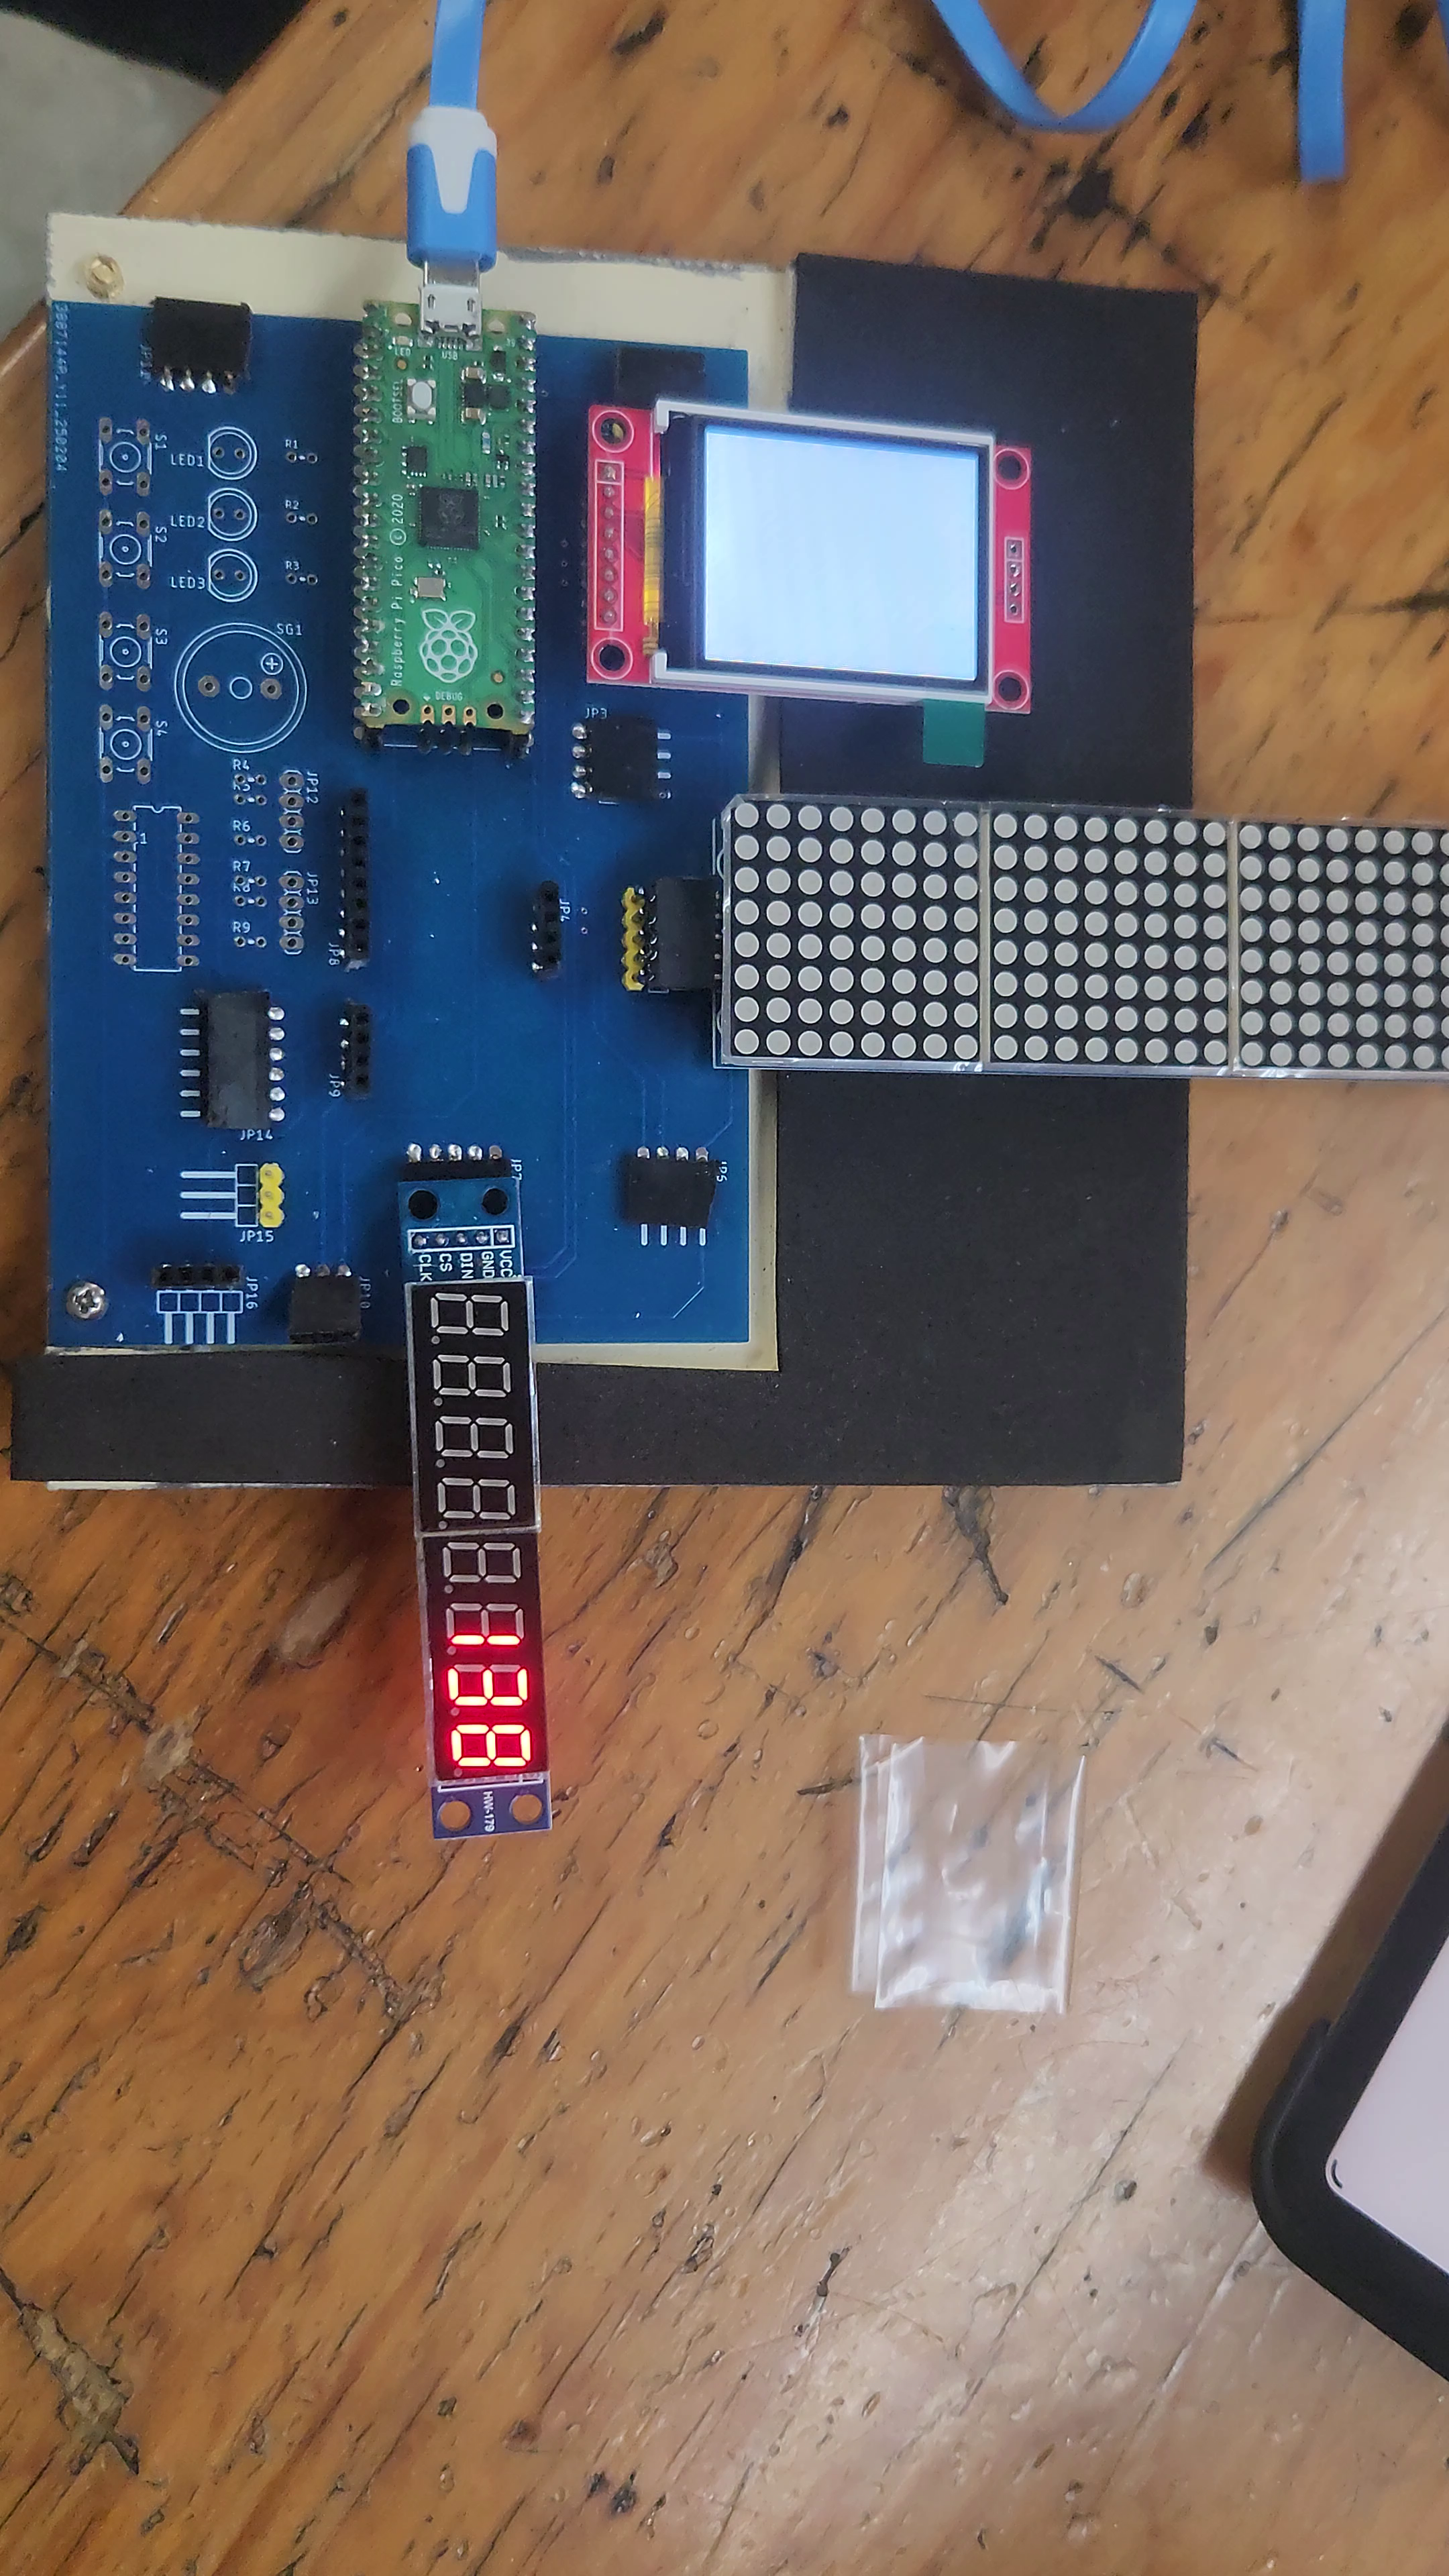
\includegraphics[width=0.6\linewidth, angle=90]{img/Actividad2/Act2_1.png}
            \caption{Actividad 2 - Contador Ascendente: \texttt{138}}
        \end{subfigure}
        \hfill
        \begin{subfigure}[b]{0.45\textwidth}
            \centering
            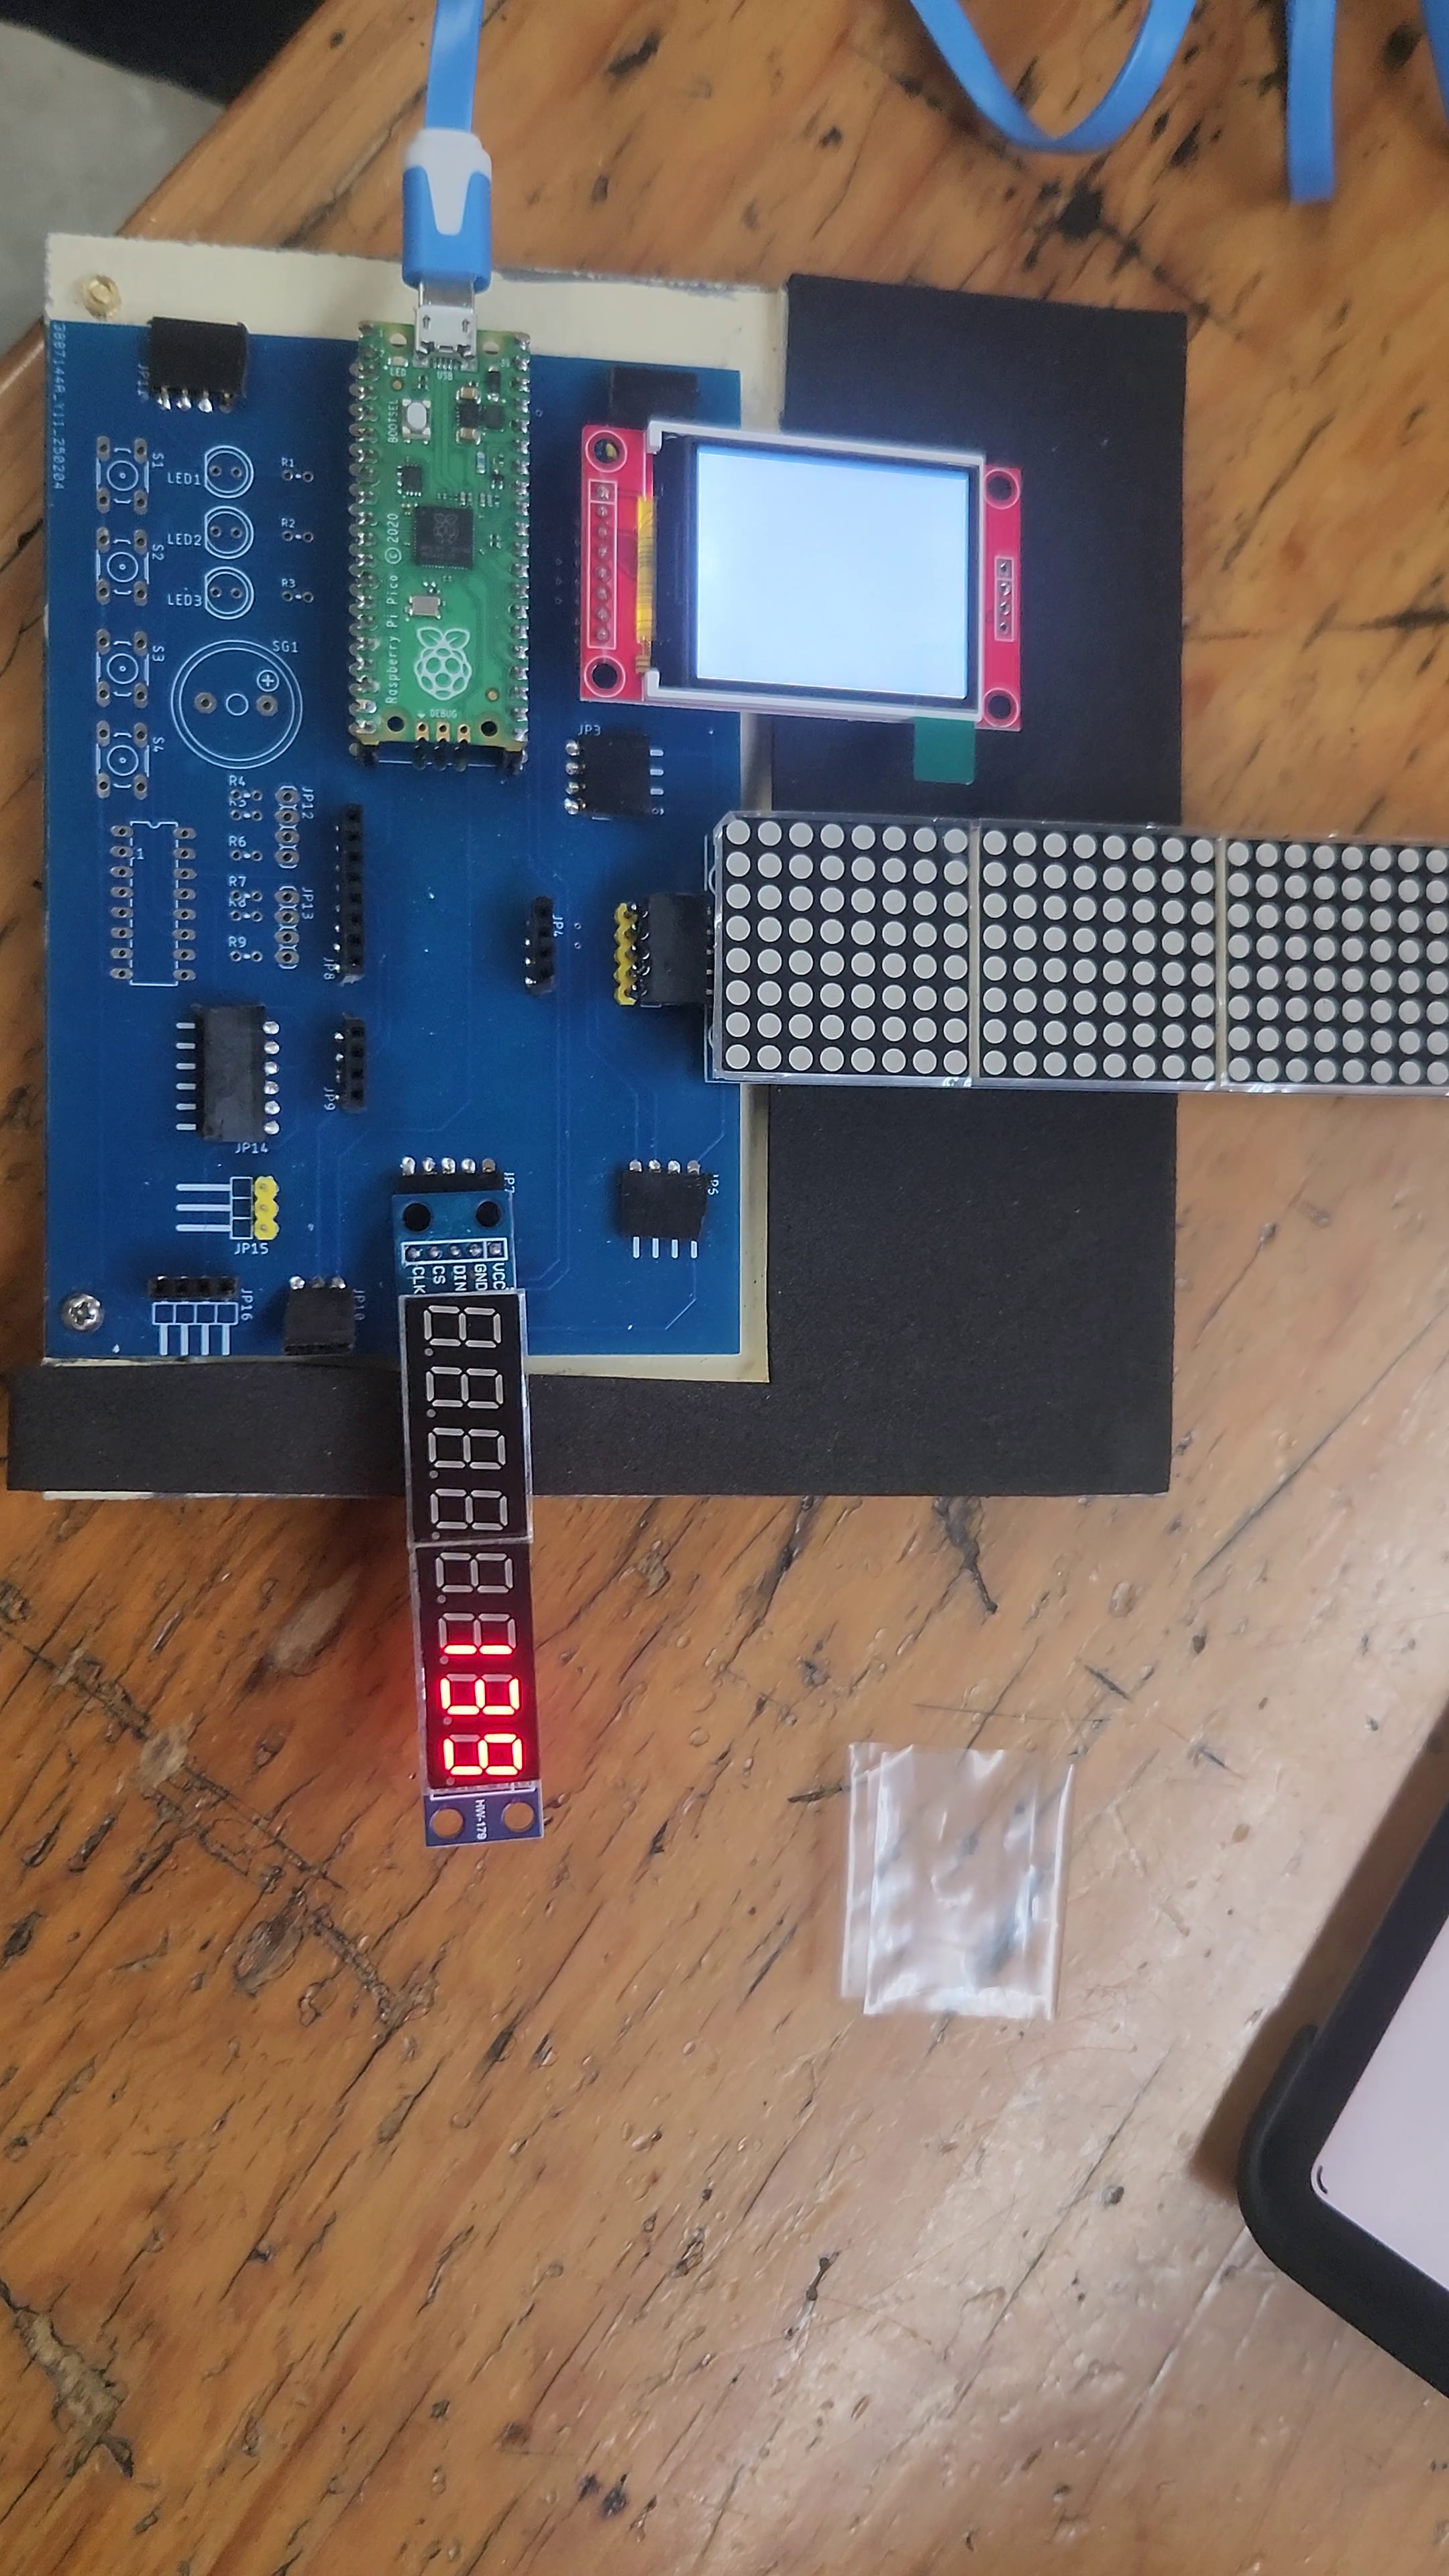
\includegraphics[width=0.55\linewidth, angle=90]{img/Actividad2/Act2_3.png}
            \caption{Actividad 2 - Contador Ascendente: \texttt{139}}
        \end{subfigure}

        \vspace{0.5cm}

        % --- FILA 2 ---
        \begin{subfigure}[b]{0.45\textwidth}
            \centering
            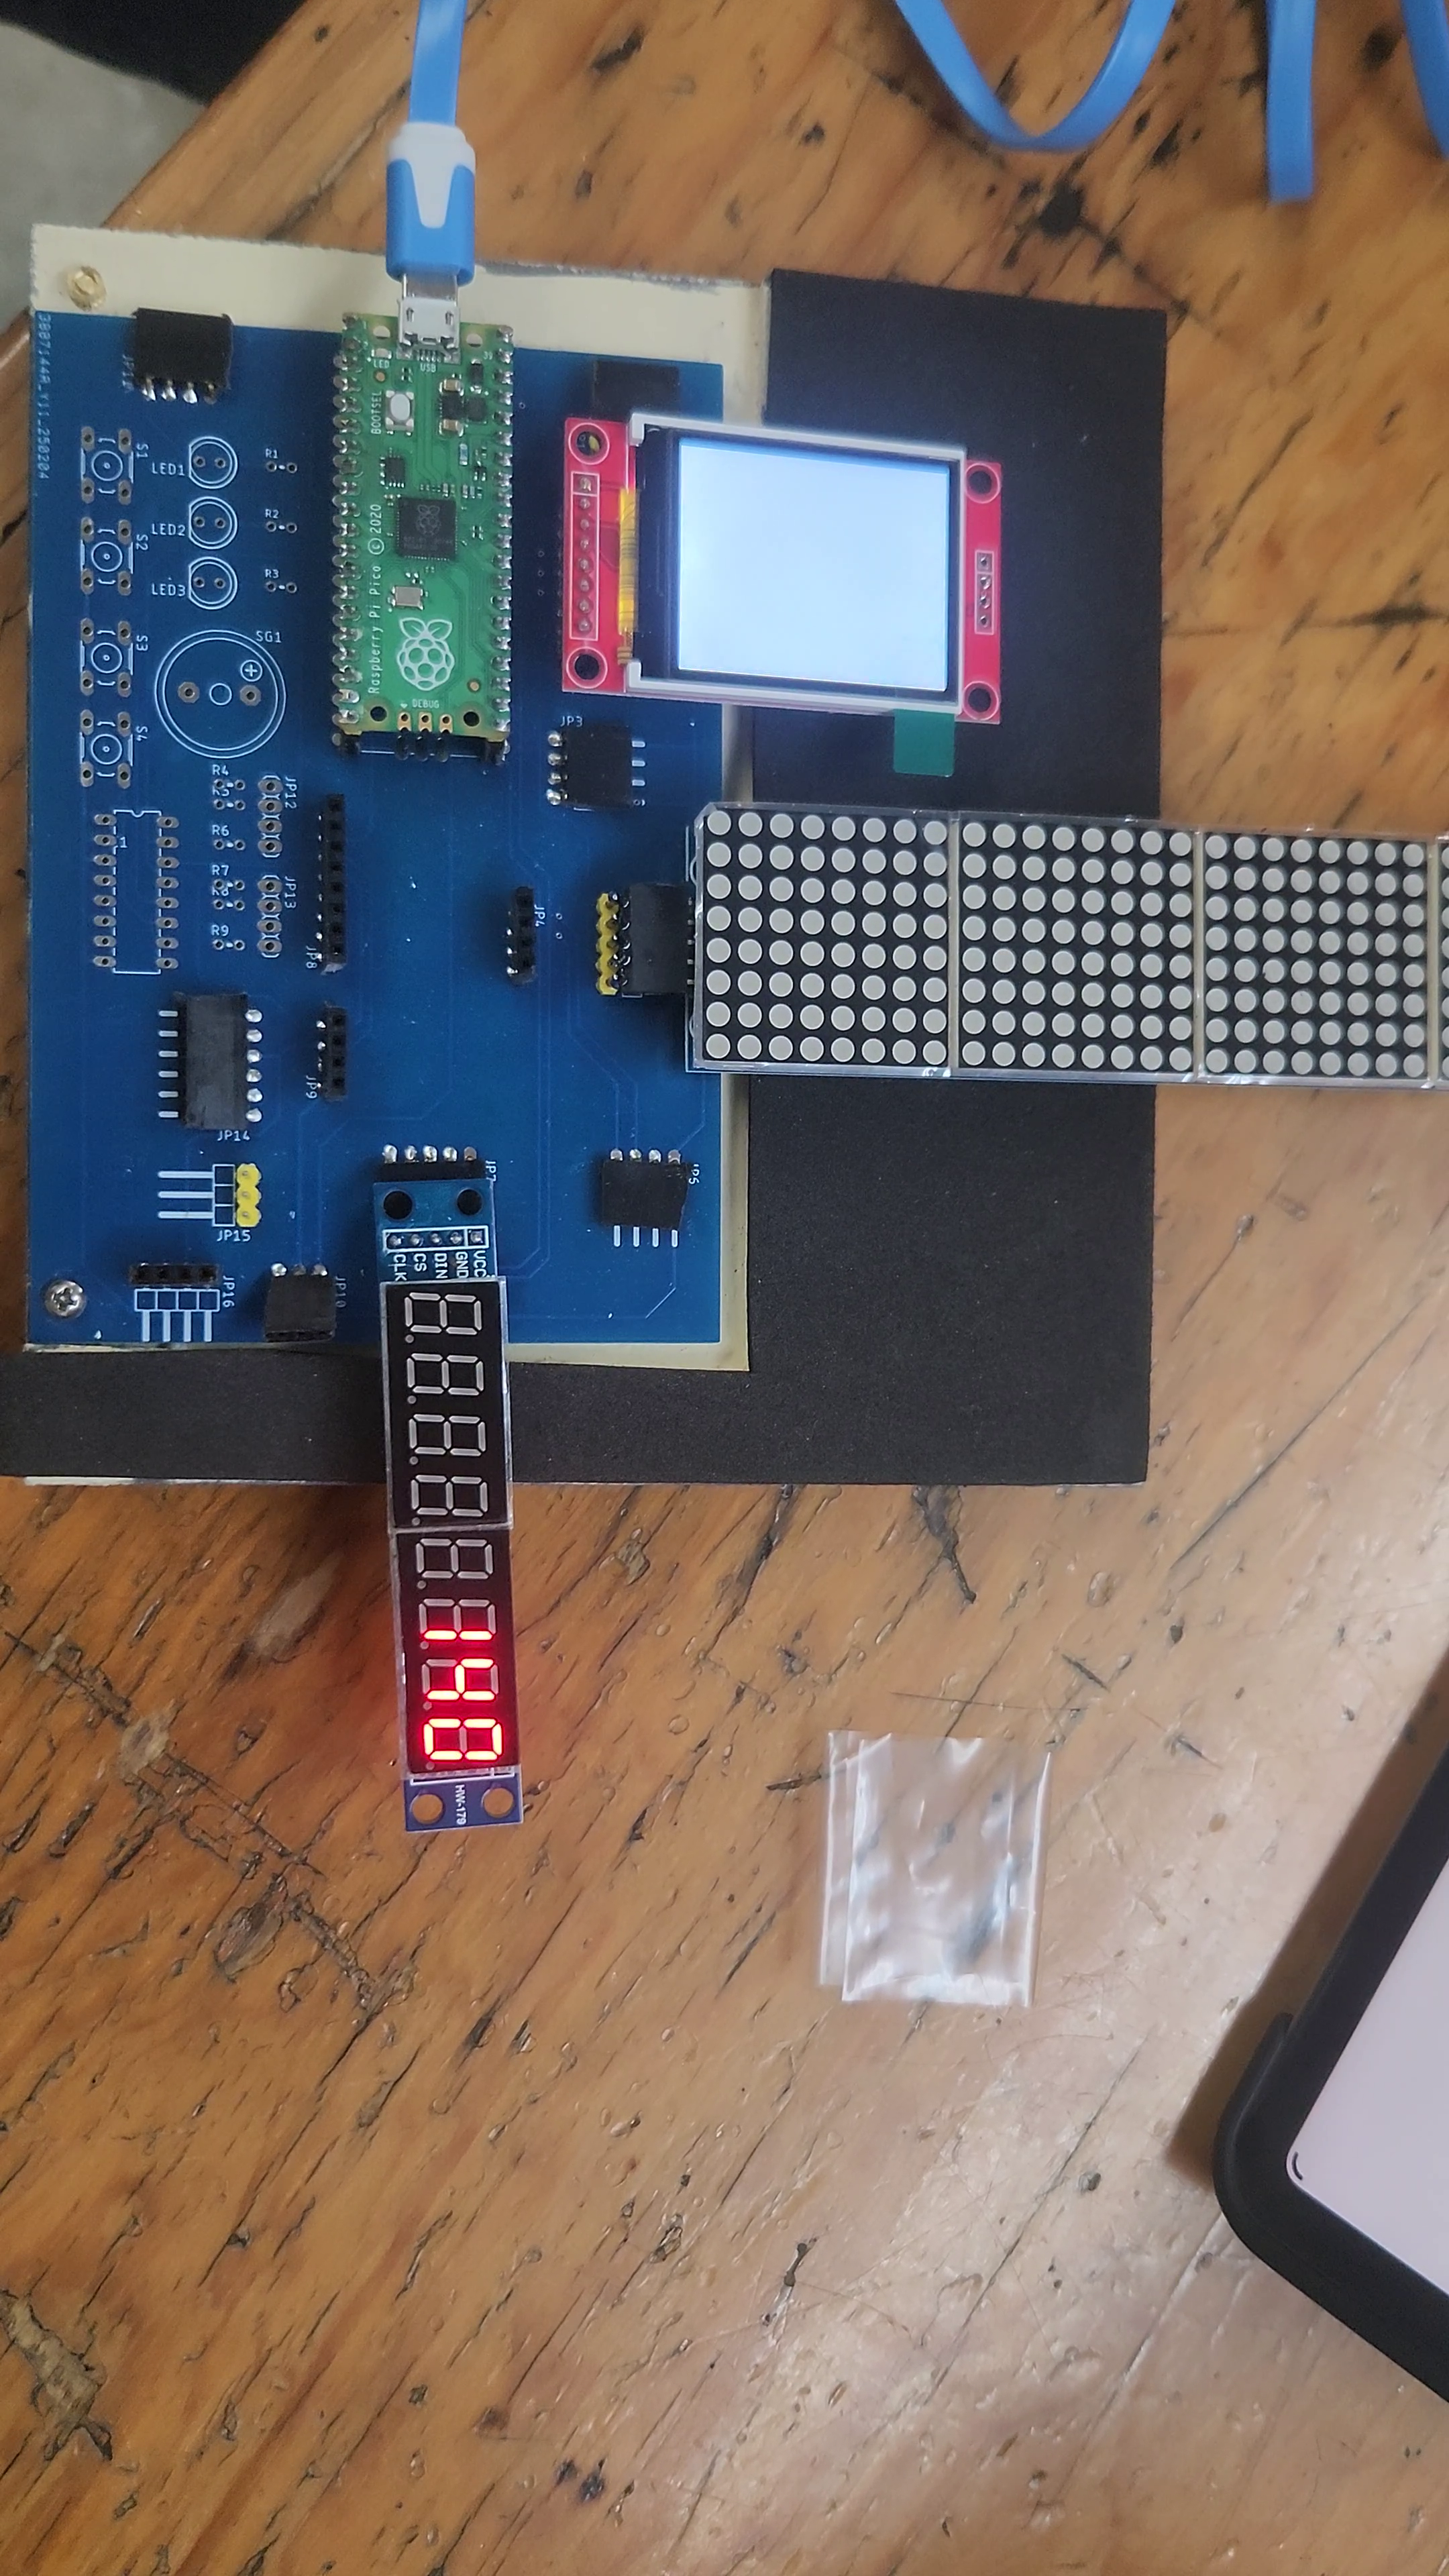
\includegraphics[width=0.55\linewidth, angle=90]{img/Actividad2/Act2_4.png}
            \caption{Actividad 2 - Contador Ascendente: \texttt{140}}
        \end{subfigure}
        \hfill
        \begin{subfigure}[b]{0.45\textwidth}
            \centering
            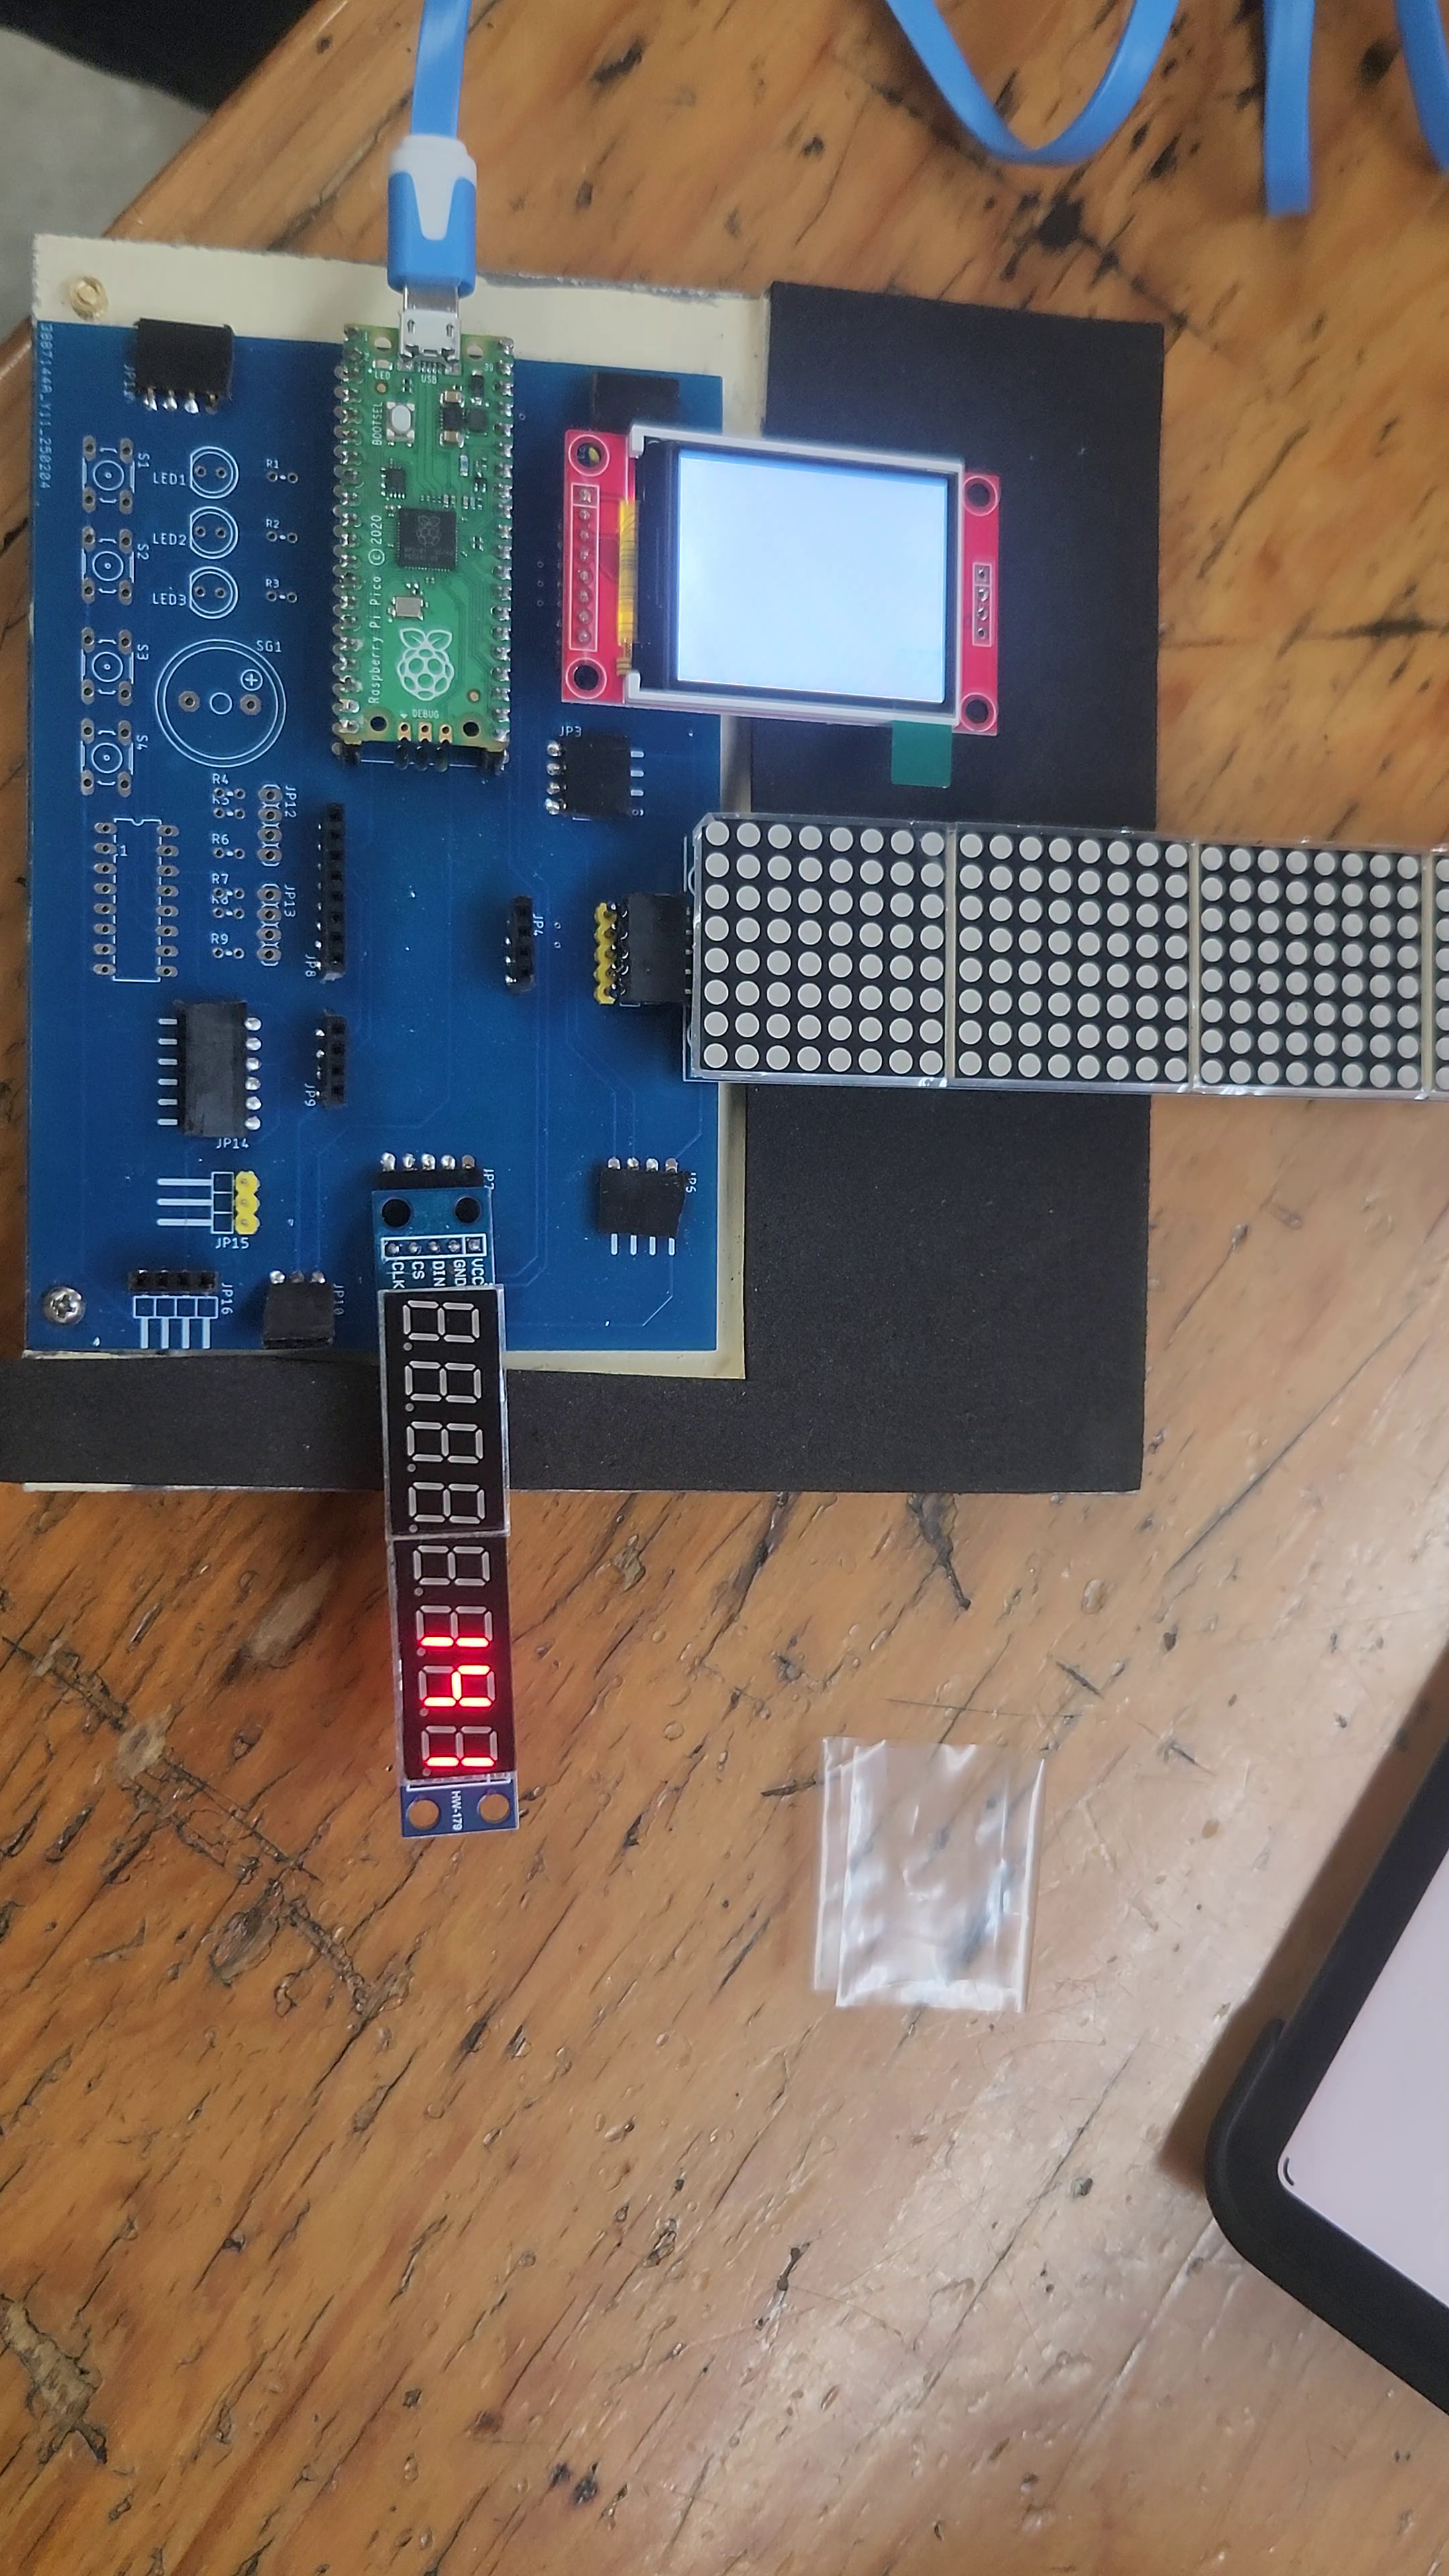
\includegraphics[width=0.55\linewidth, angle=90]{img/Actividad2/Act2_5.png}
            \caption{Actividad 2 - Contador Ascendente: \texttt{141}}
        \end{subfigure}

        \vspace{0.5cm}

        % --- FILA 3 ---
        \begin{subfigure}[b]{0.45\textwidth}
            \centering
            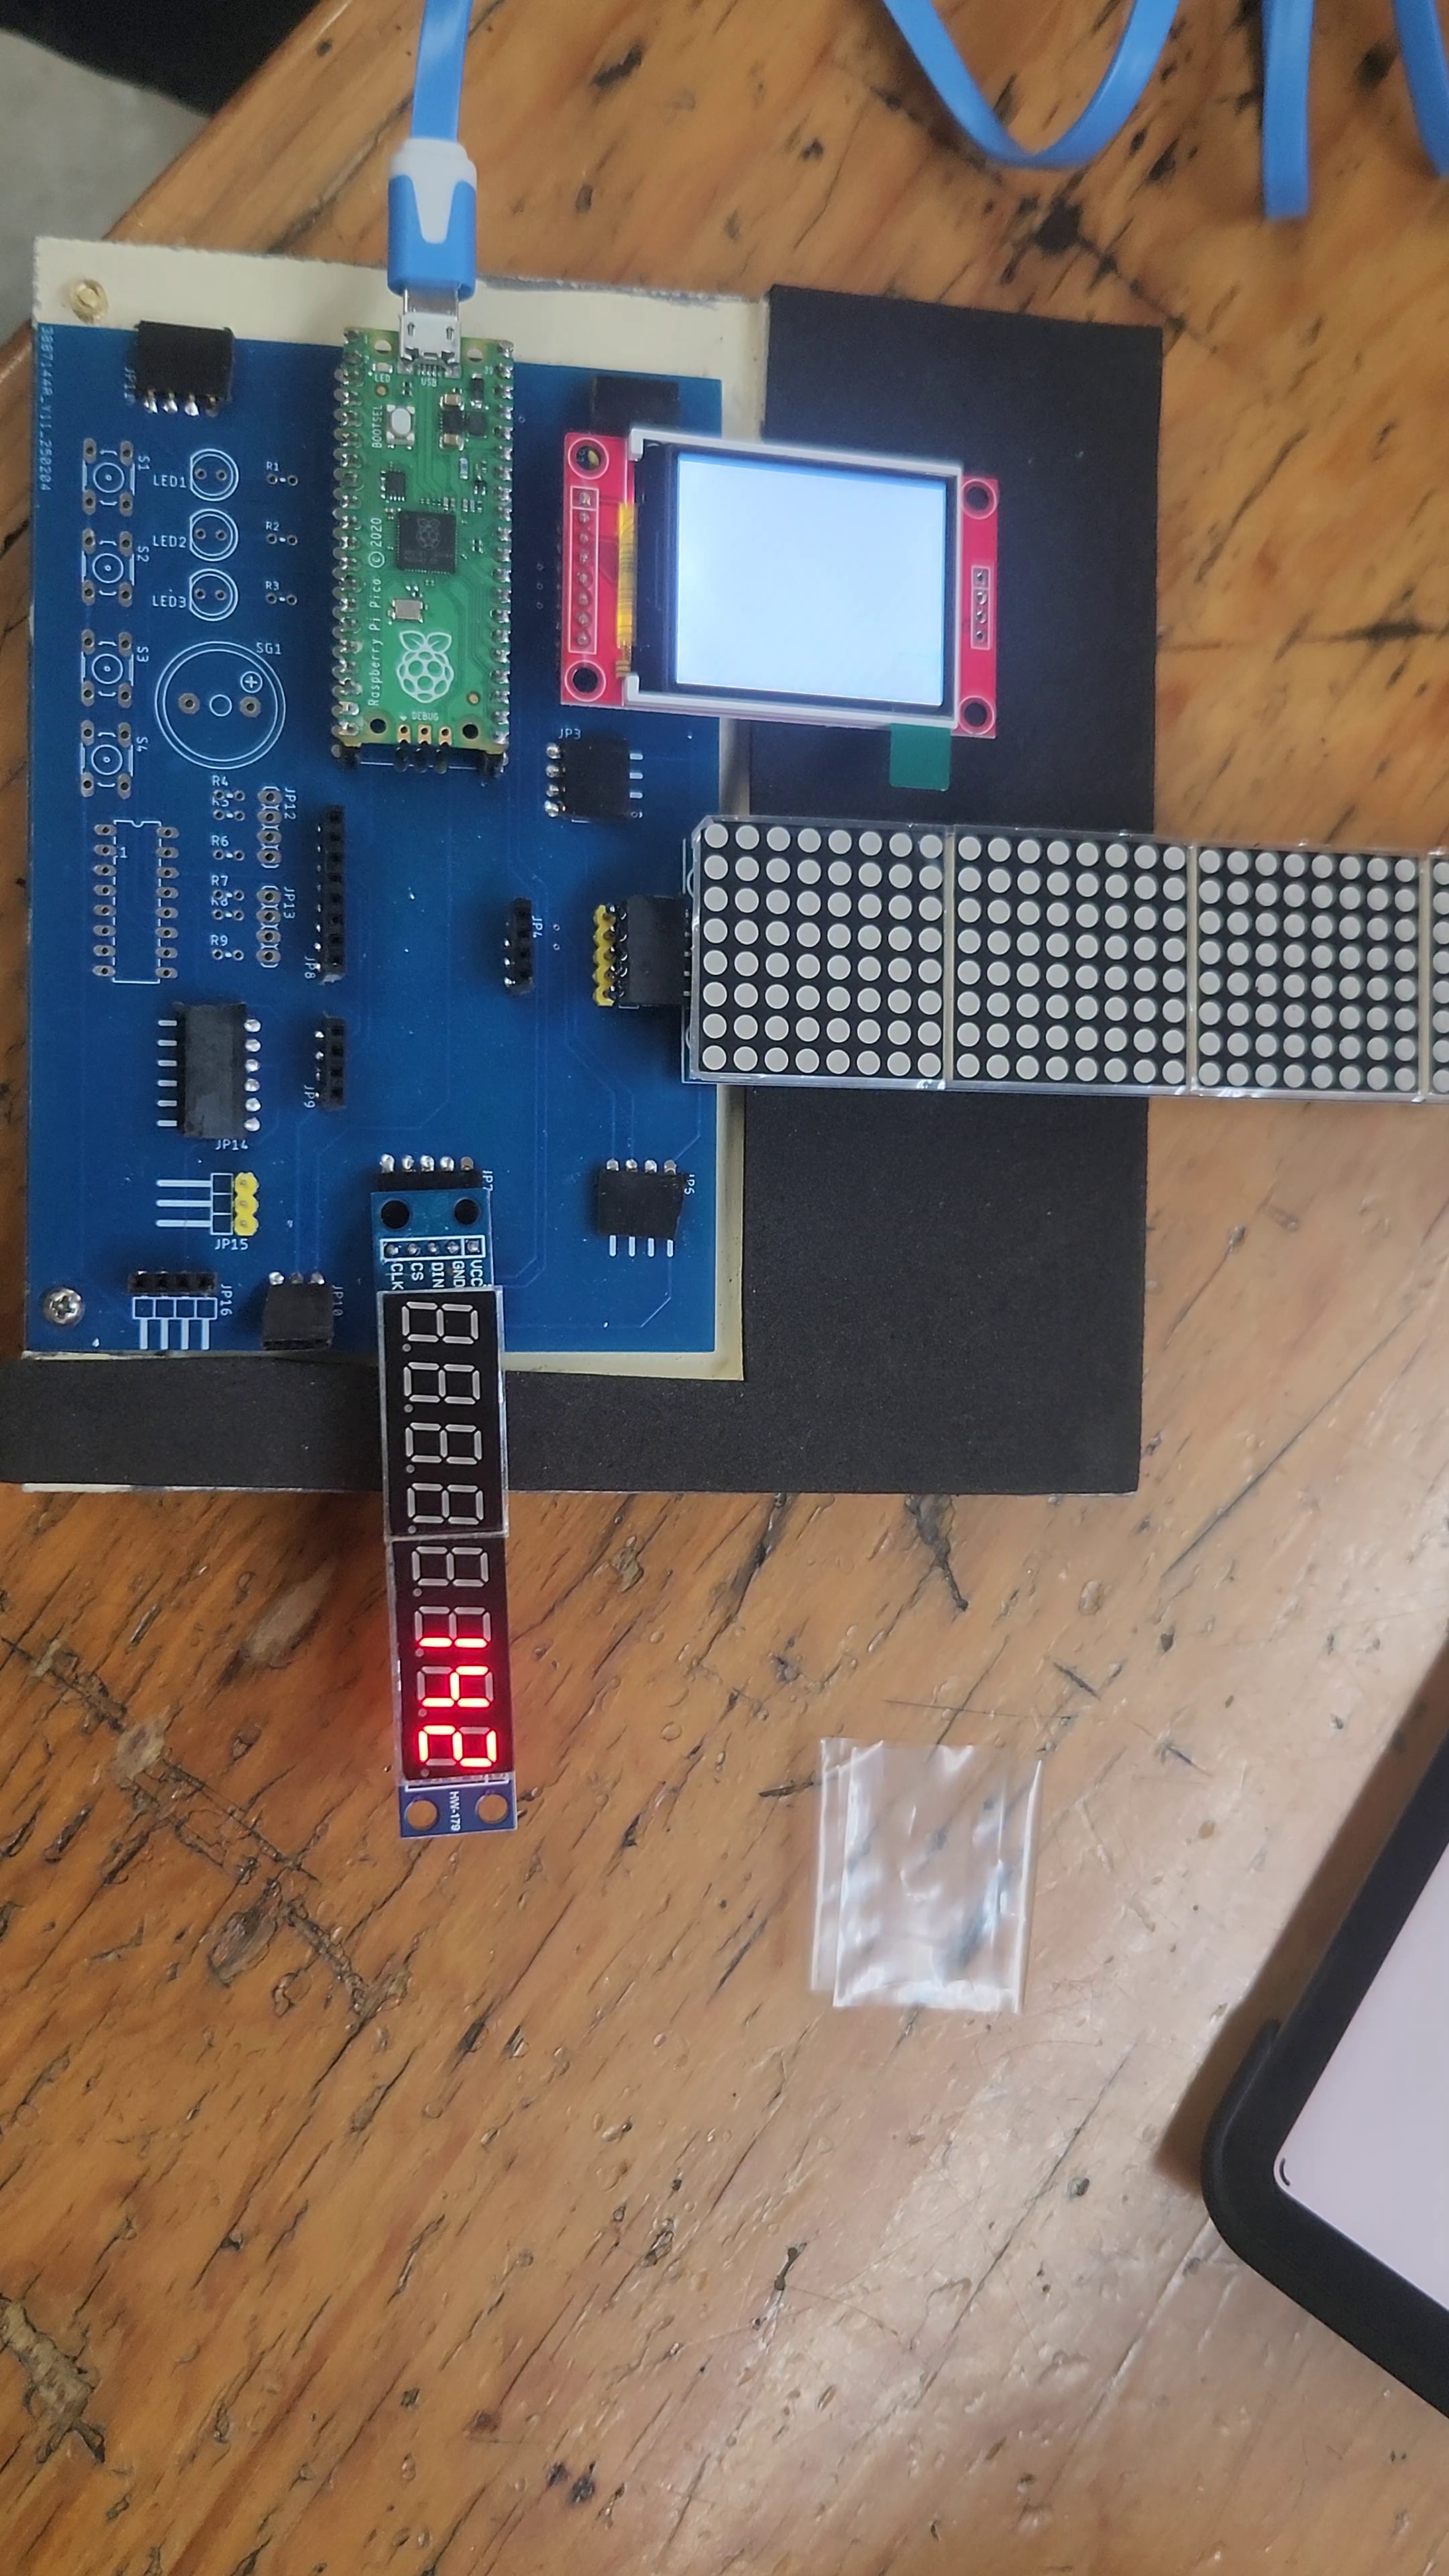
\includegraphics[width=0.55\linewidth, angle=90]{img/Actividad2/Act2_6.png}
            \caption{Actividad 2 - Contador Ascendente: \texttt{142}}
        \end{subfigure}
        \hfill
        \begin{subfigure}[b]{0.45\textwidth}
            \centering
            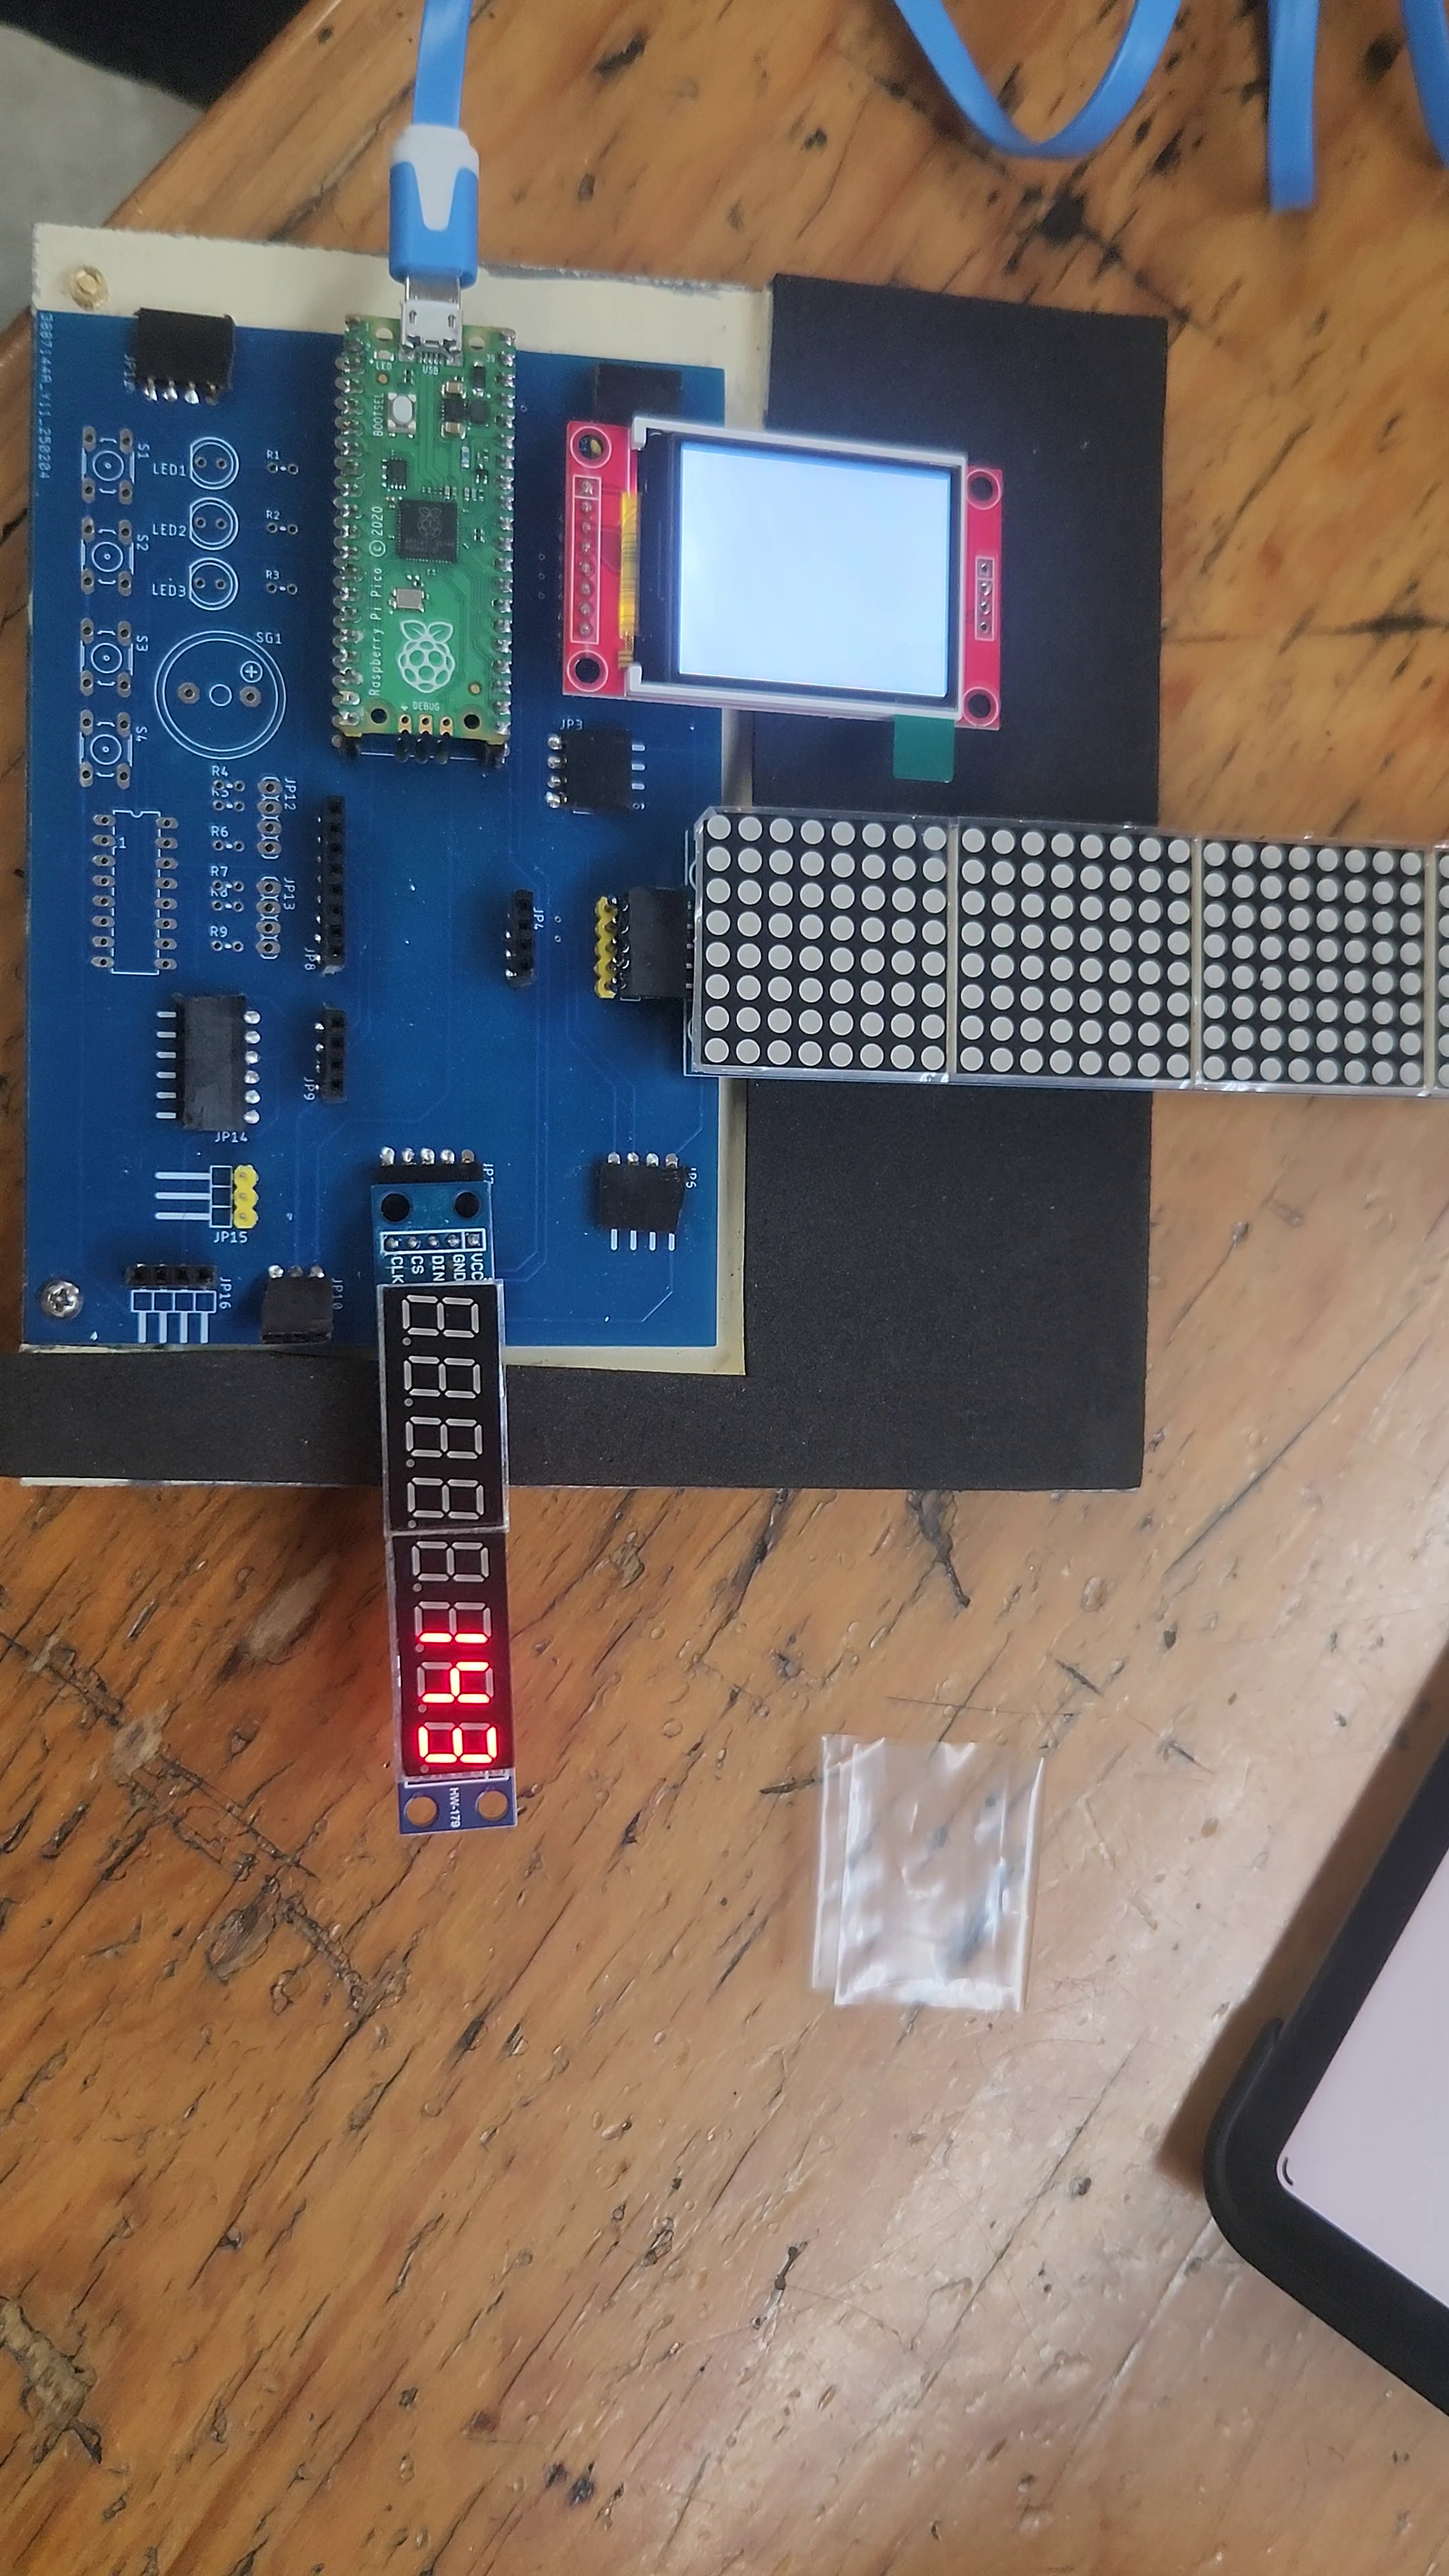
\includegraphics[width=0.55\linewidth, angle=90]{img/Actividad2/Act2_7.png}
            \caption{Actividad 2 - Contador Ascendente: \texttt{143}}
        \end{subfigure}
        \caption{Actividad 2 - Contador Ascendente.}
    \end{figure}


    \begin{figure}[htbp]
        \centering
        % --- FILA 1 ---
        \begin{subfigure}[b]{0.45\textwidth}
            \centering
            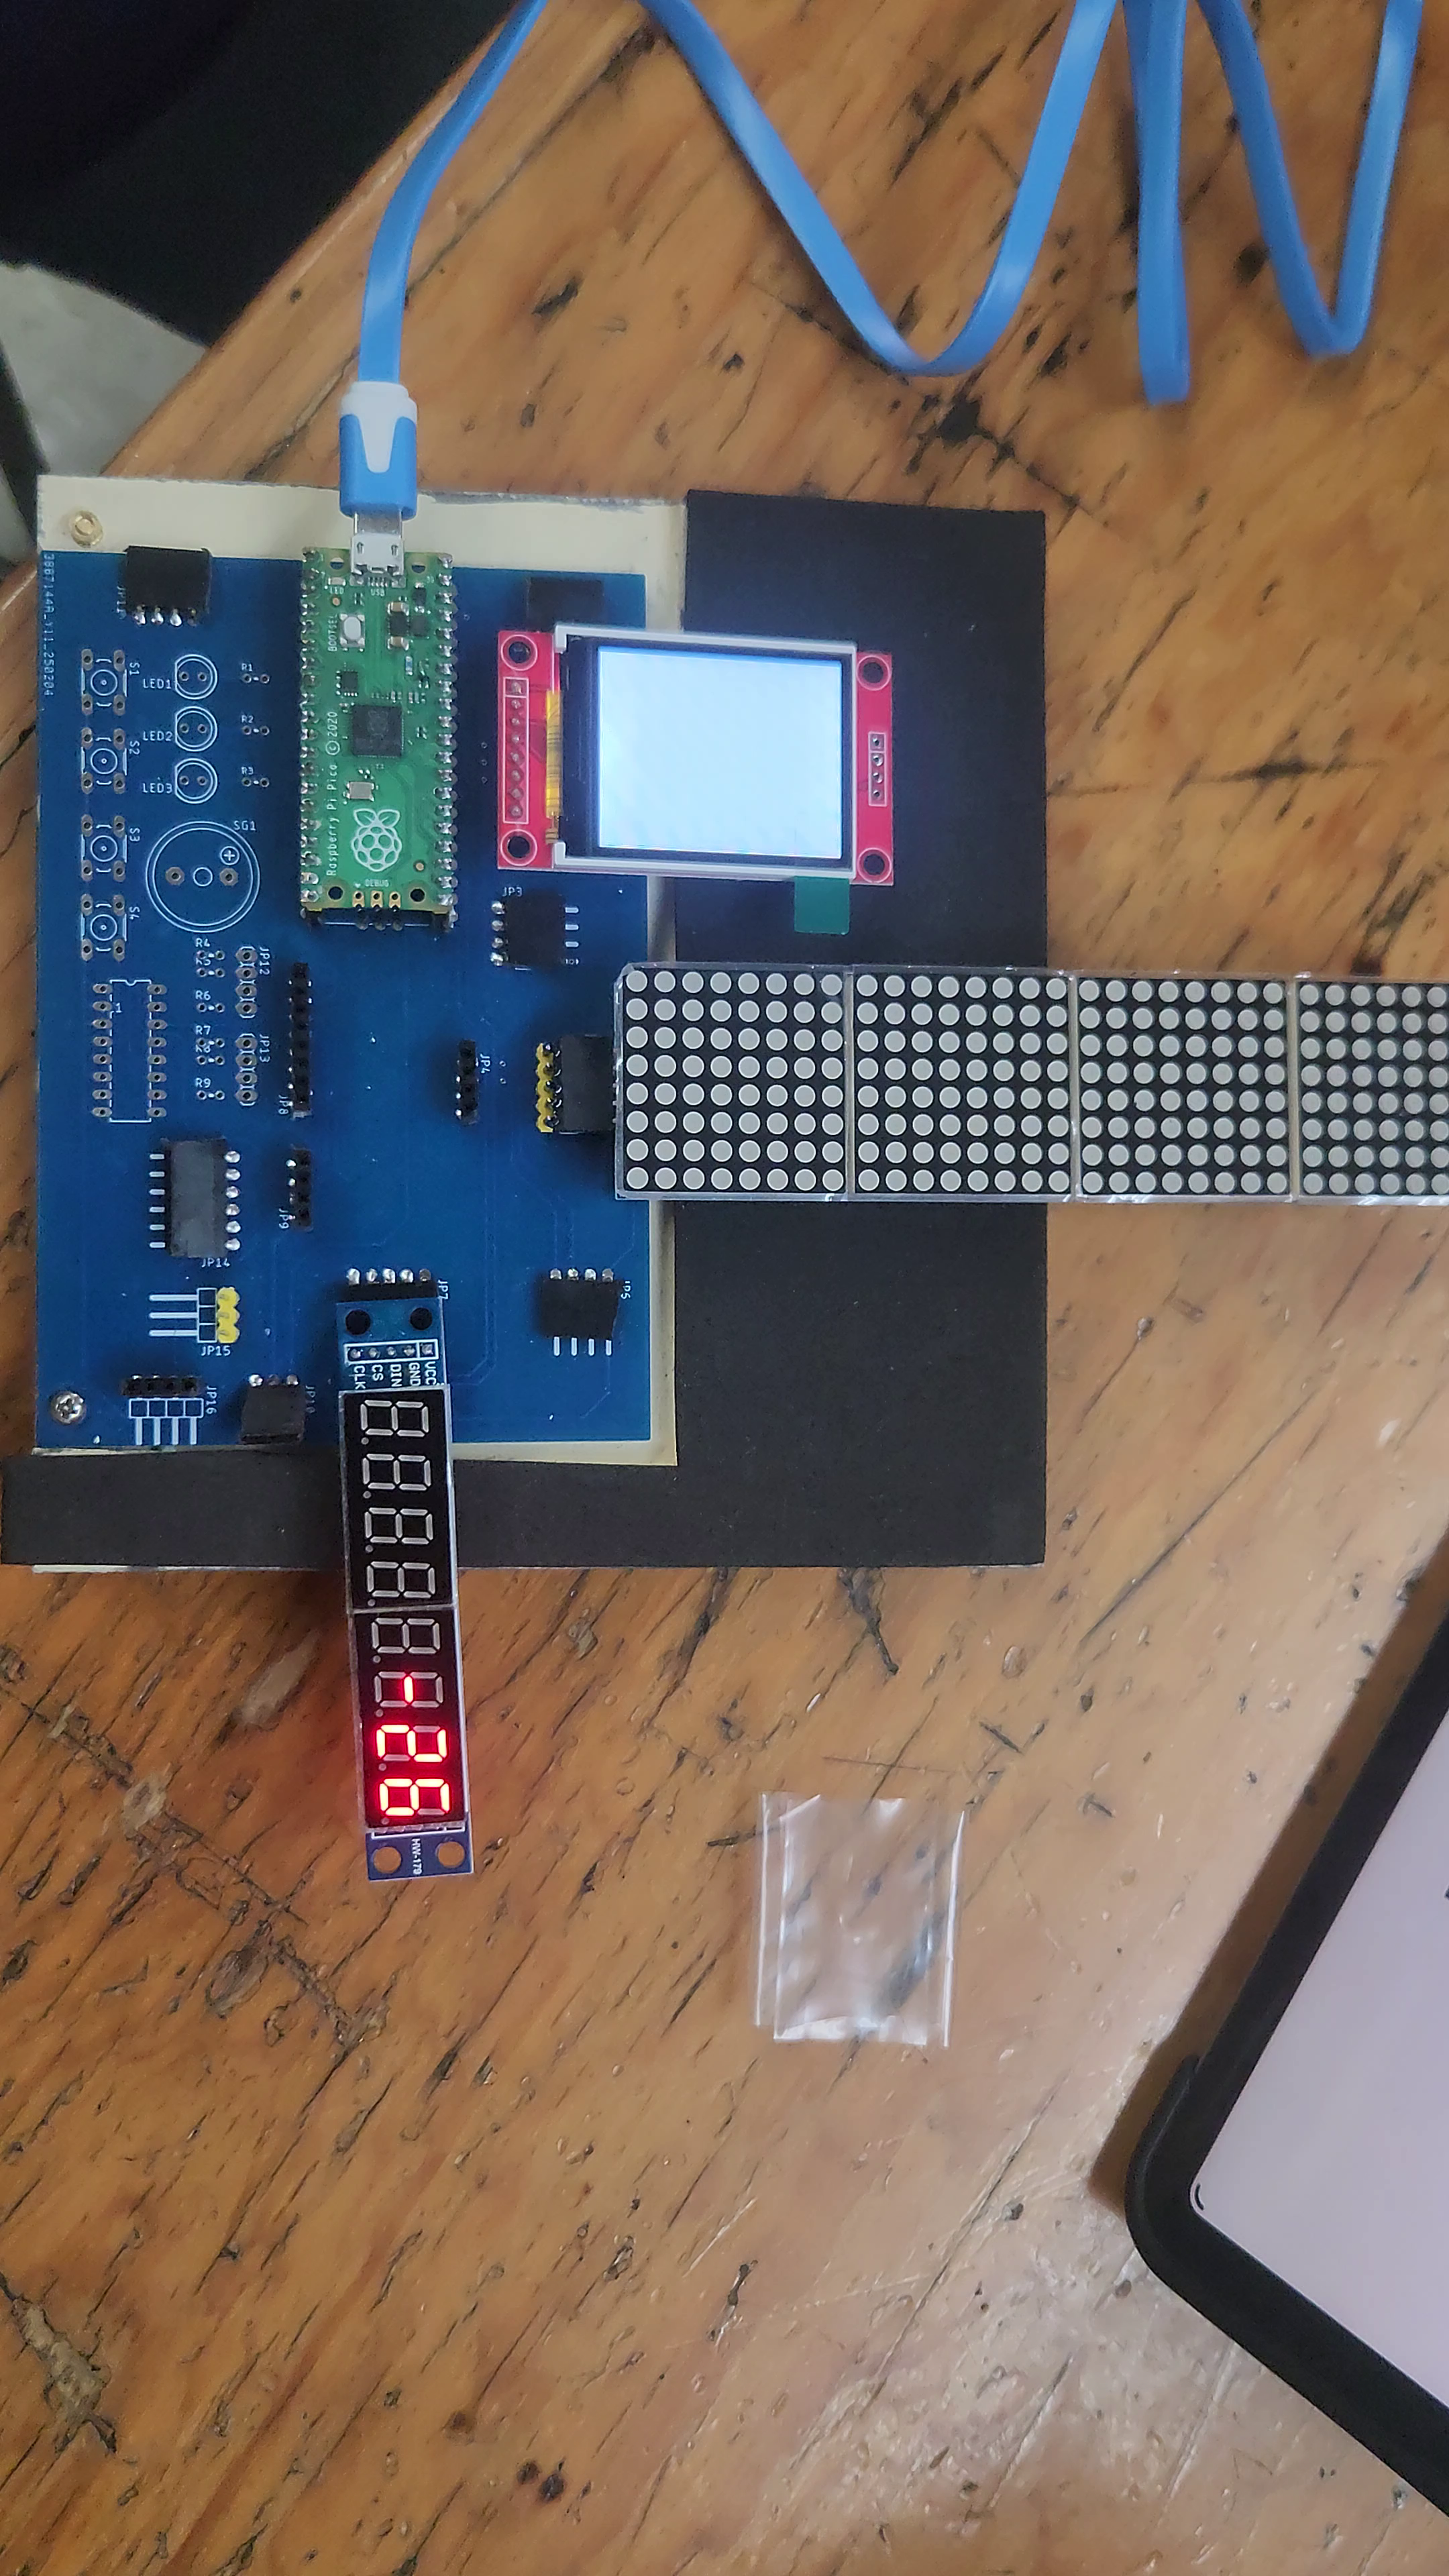
\includegraphics[width=0.6\linewidth, angle=90]{img/Actividad2/Act2_8.png}
            \caption{Actividad 2 - Contador Descendente: \texttt{-26}}
        \end{subfigure}
        \hfill
        \begin{subfigure}[b]{0.45\textwidth}
            \centering
            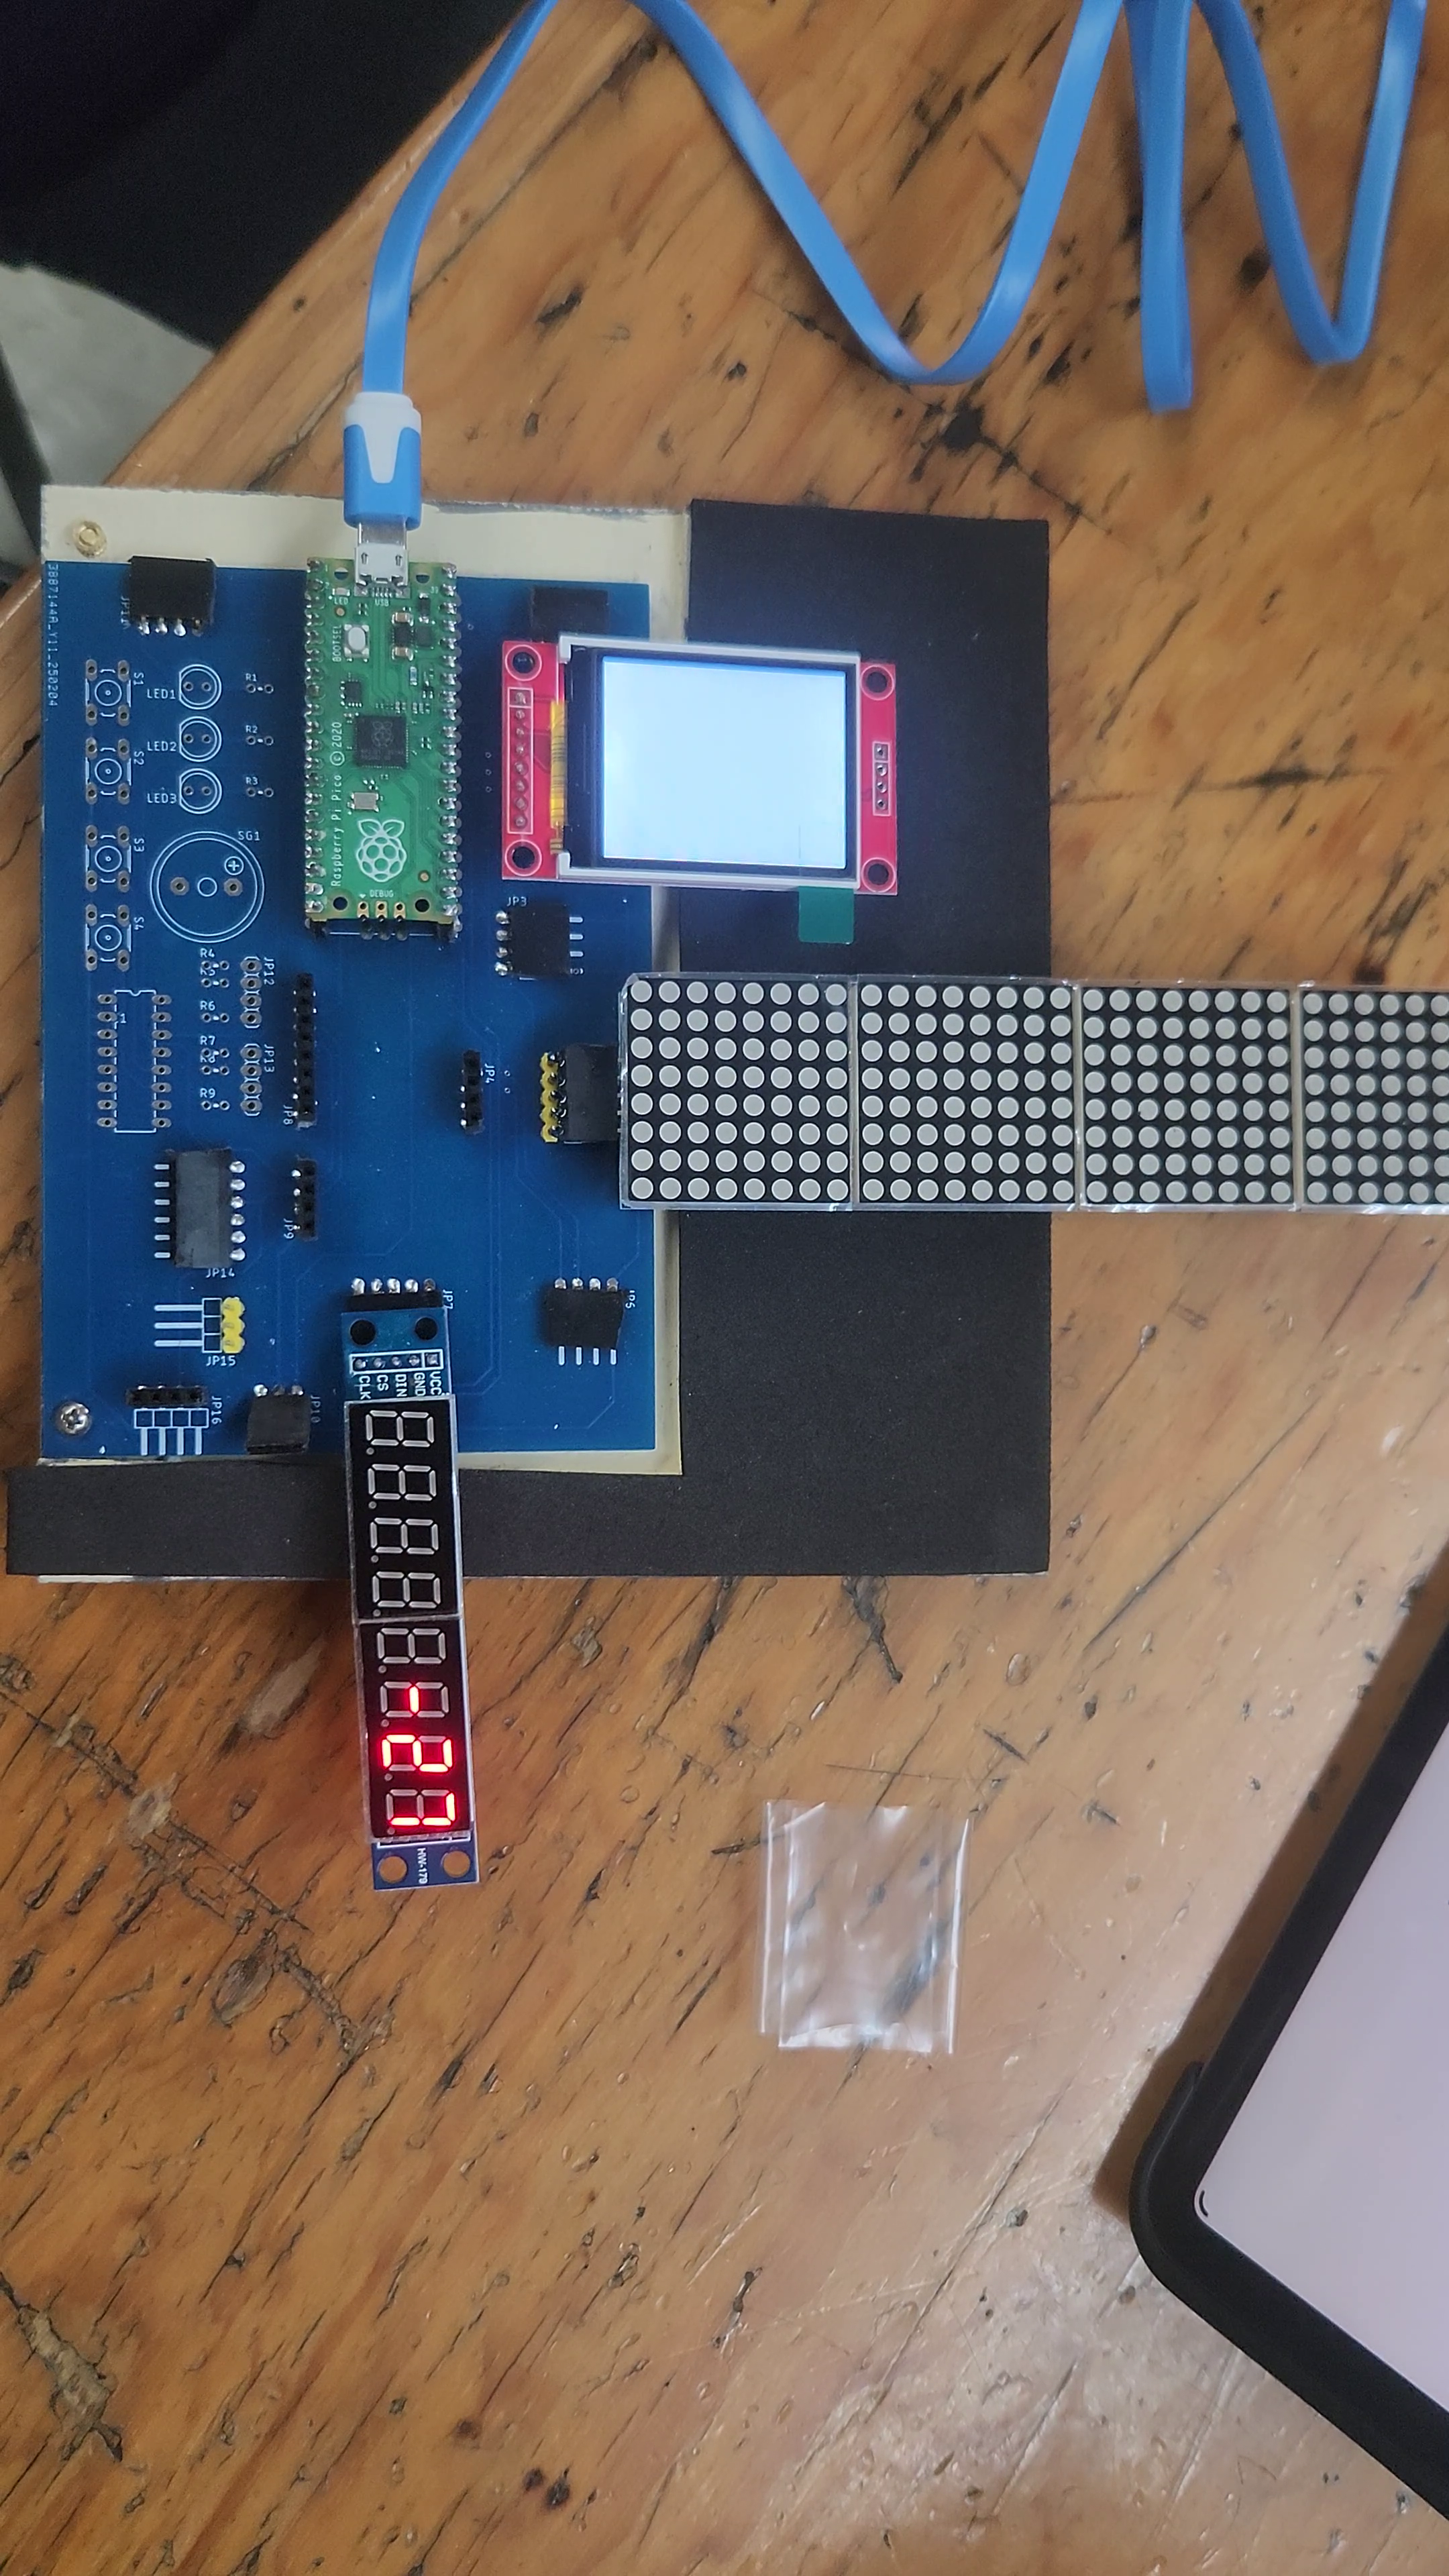
\includegraphics[width=0.55\linewidth, angle=90]{img/Actividad2/Act2_9.png}
            \caption{Actividad 2 - Contador Descendente: \texttt{-27}}
        \end{subfigure}

        \vspace{0.5cm}

        % --- FILA 2 ---
        \begin{subfigure}[b]{0.45\textwidth}
            \centering
            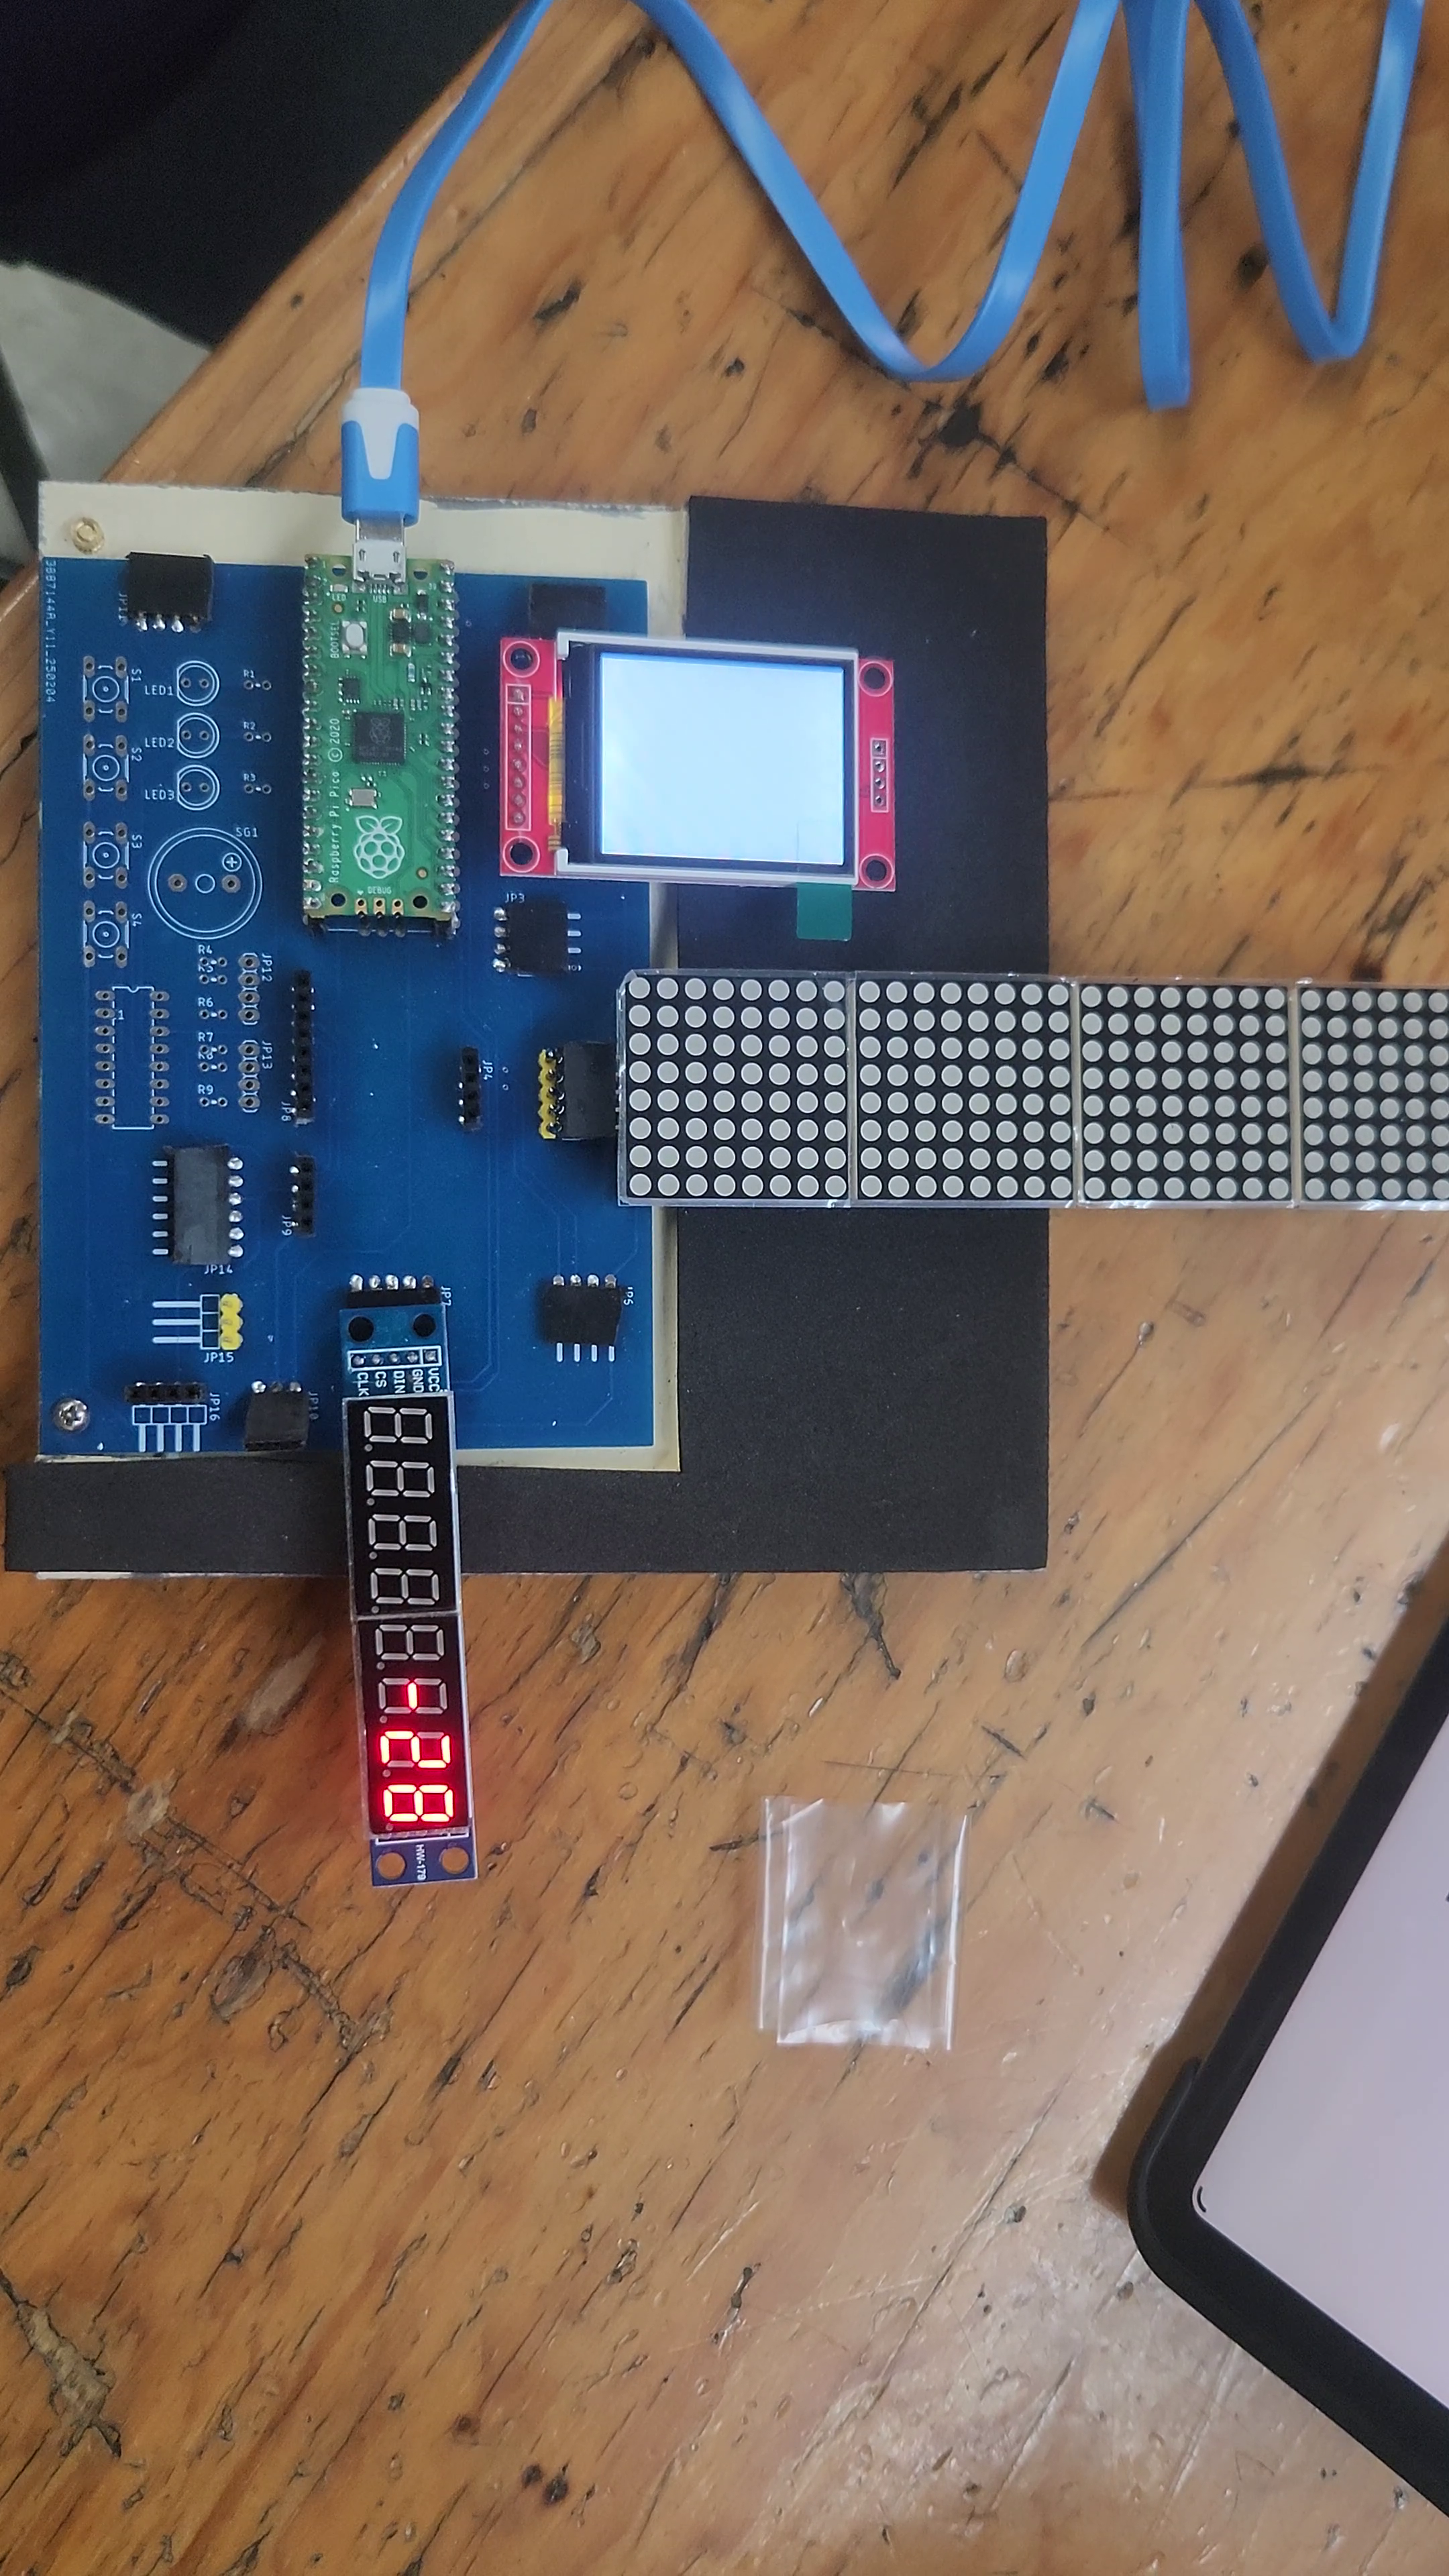
\includegraphics[width=0.55\linewidth, angle=90]{img/Actividad2/Act2_10.png}
            \caption{Actividad 2 - Contador Descendente: \texttt{-28}}
        \end{subfigure}
        \hfill
        \begin{subfigure}[b]{0.45\textwidth}
            \centering
            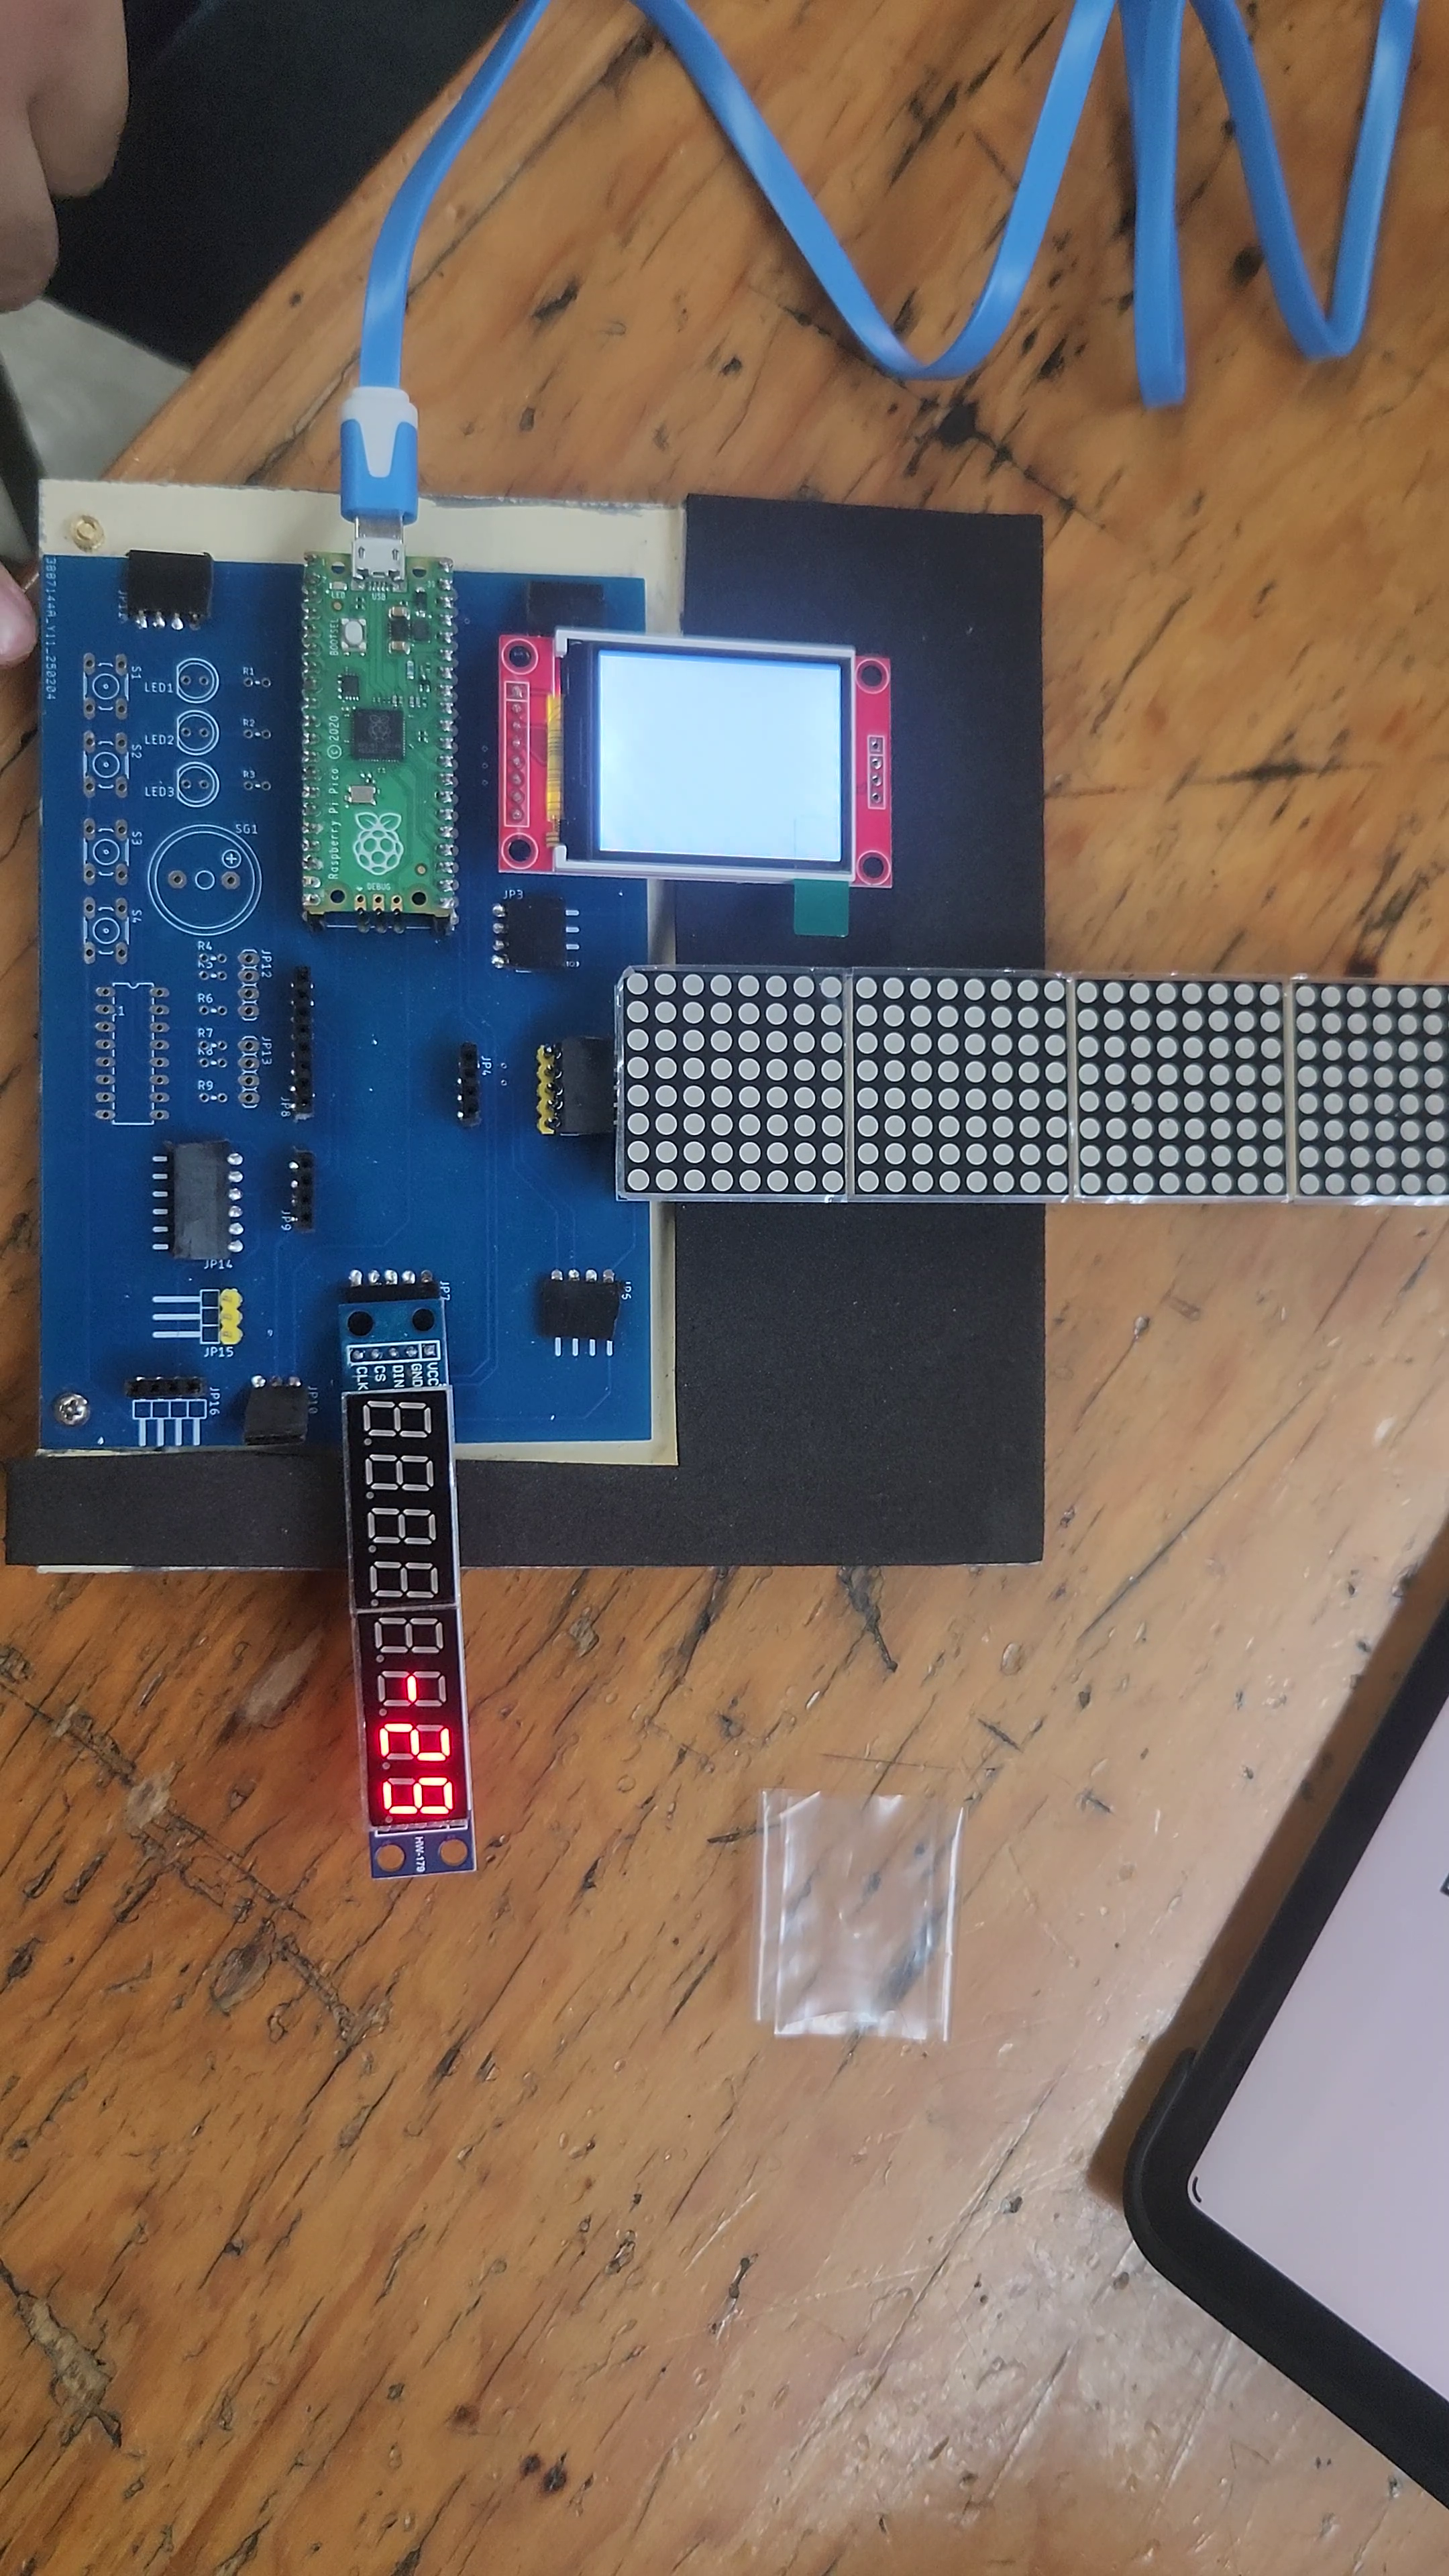
\includegraphics[width=0.55\linewidth, angle=90]{img/Actividad2/Act2_11.png}
            \caption{Actividad 2 - Contador Descendente: \texttt{-29}}
        \end{subfigure}

        \vspace{0.5cm}

        % --- FILA 3 ---
        \begin{subfigure}[b]{0.45\textwidth}
            \centering
            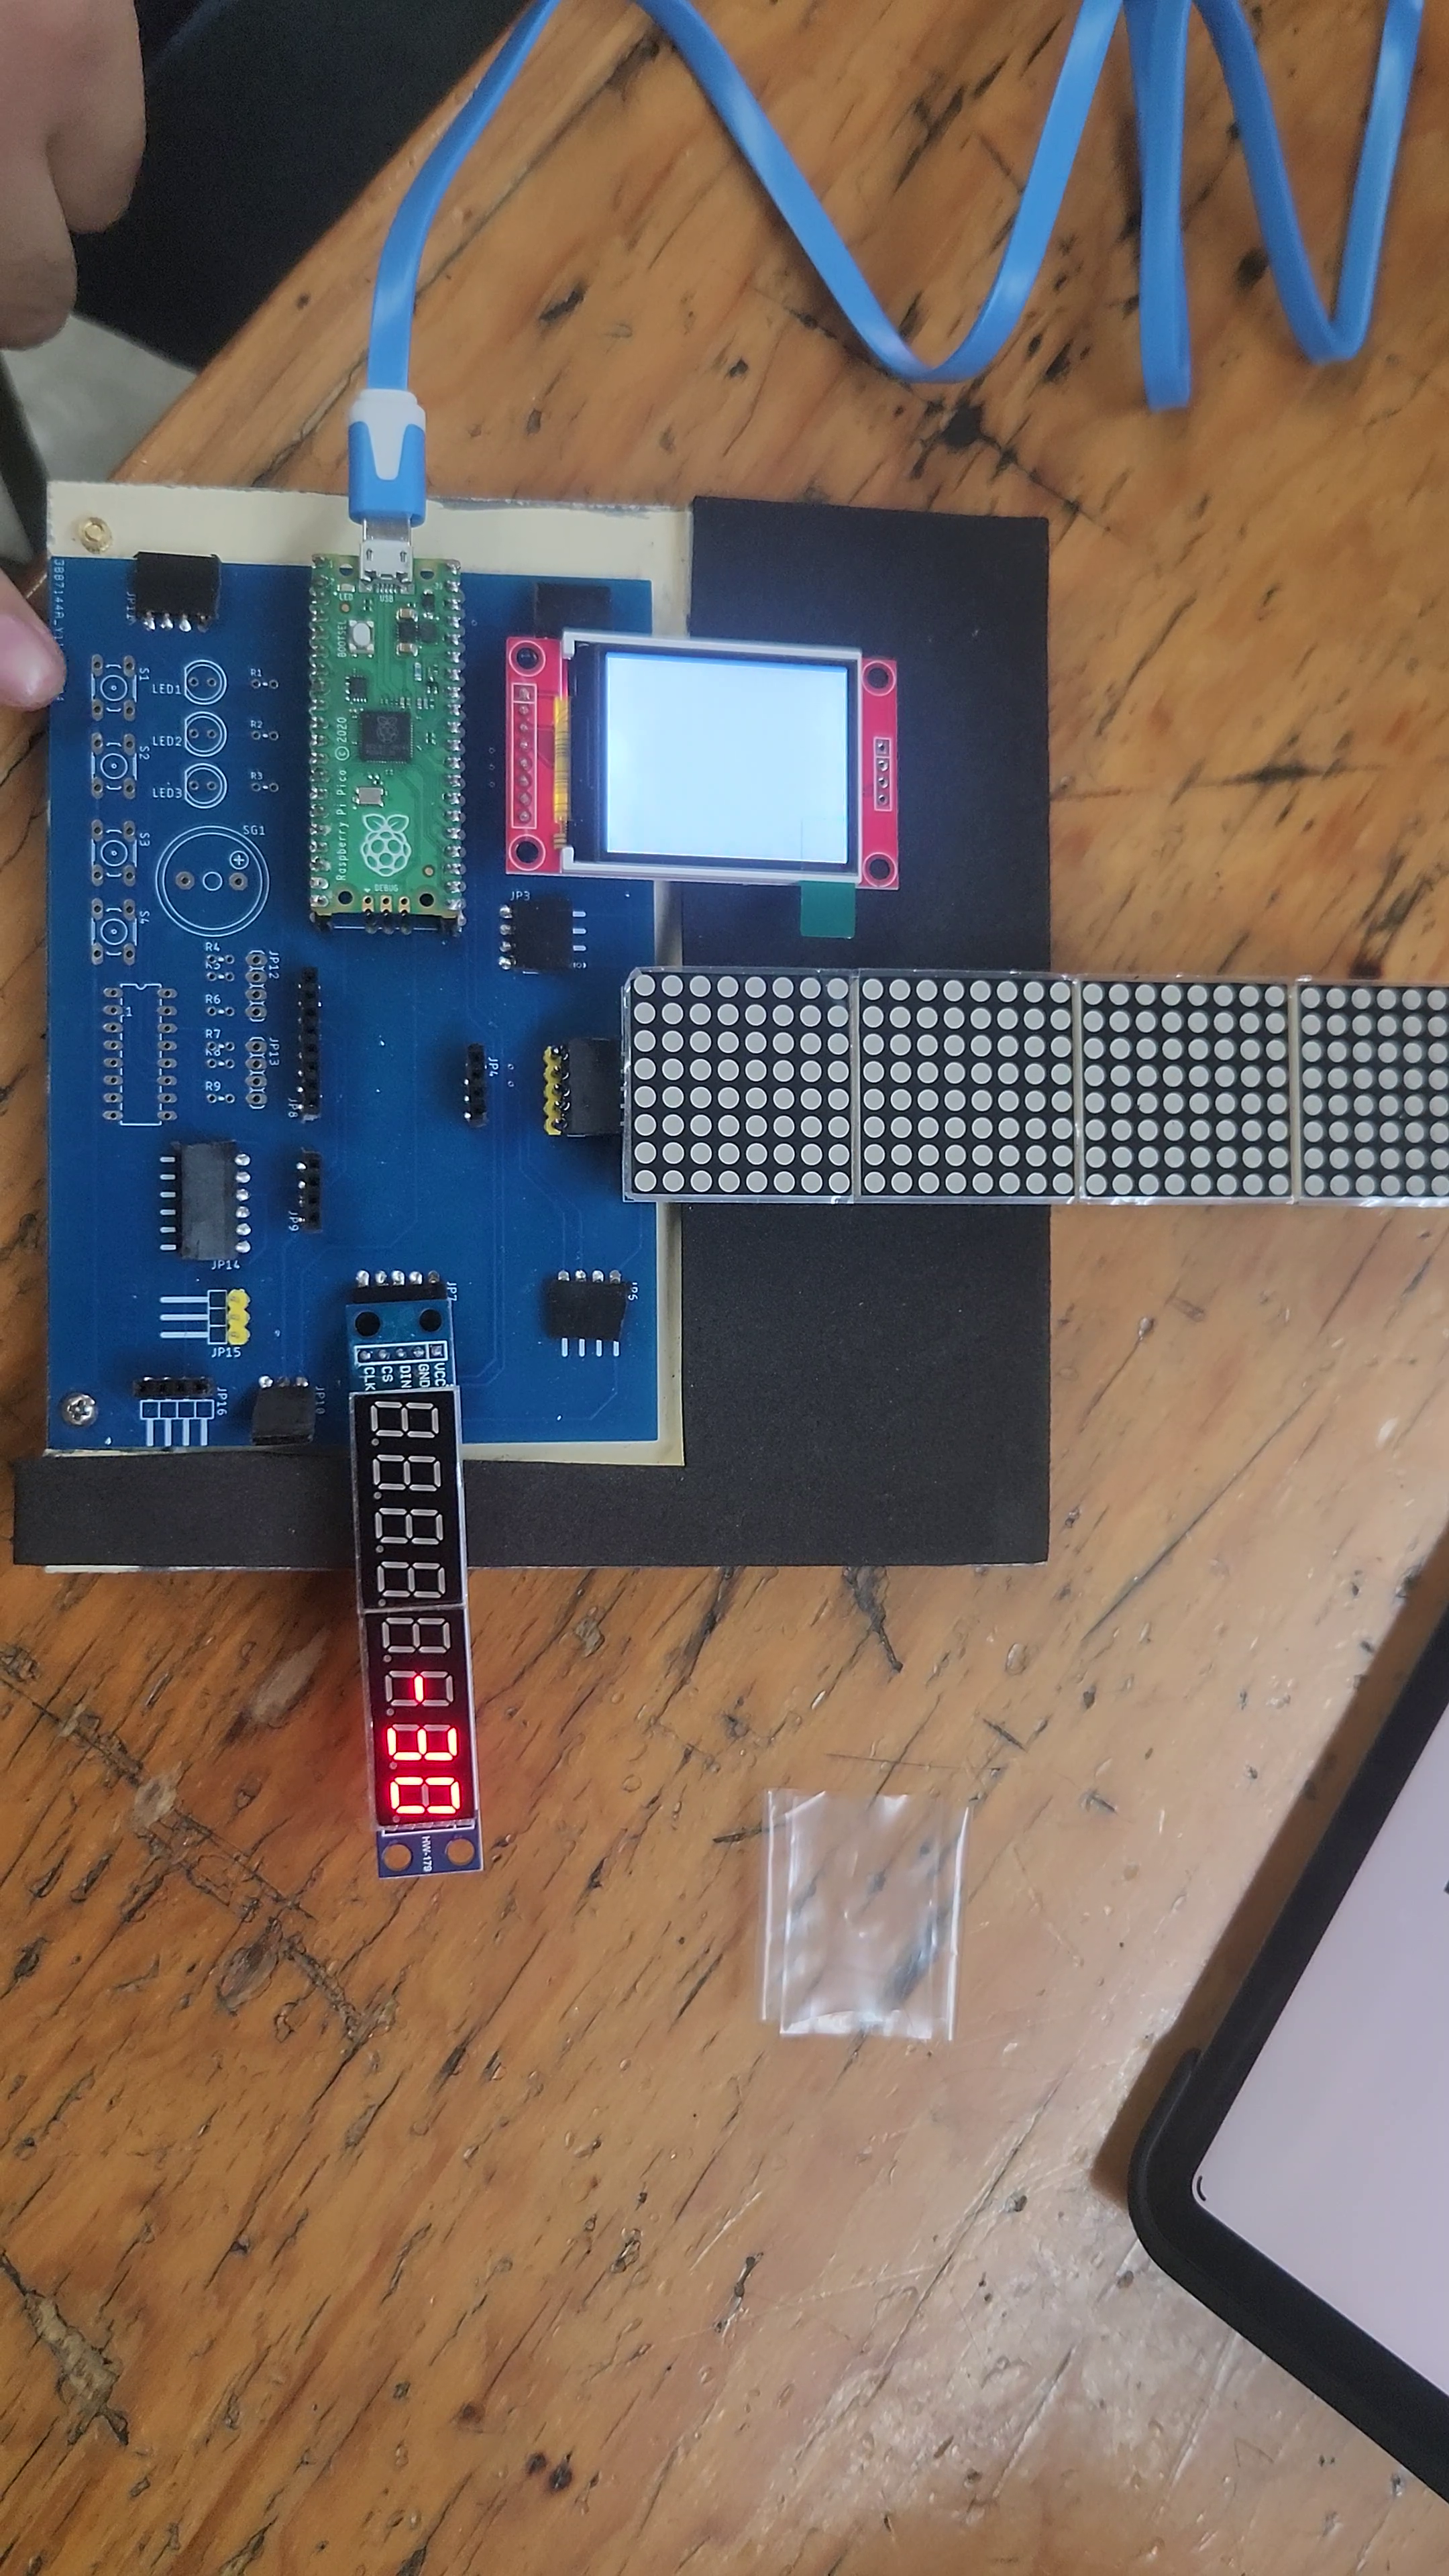
\includegraphics[width=0.55\linewidth, angle=90]{img/Actividad2/Act2_12.png}
            \caption{Actividad 2 - Contador Descendente: \texttt{-30}}
        \end{subfigure}
        \hfill
        \begin{subfigure}[b]{0.45\textwidth}
            \centering
            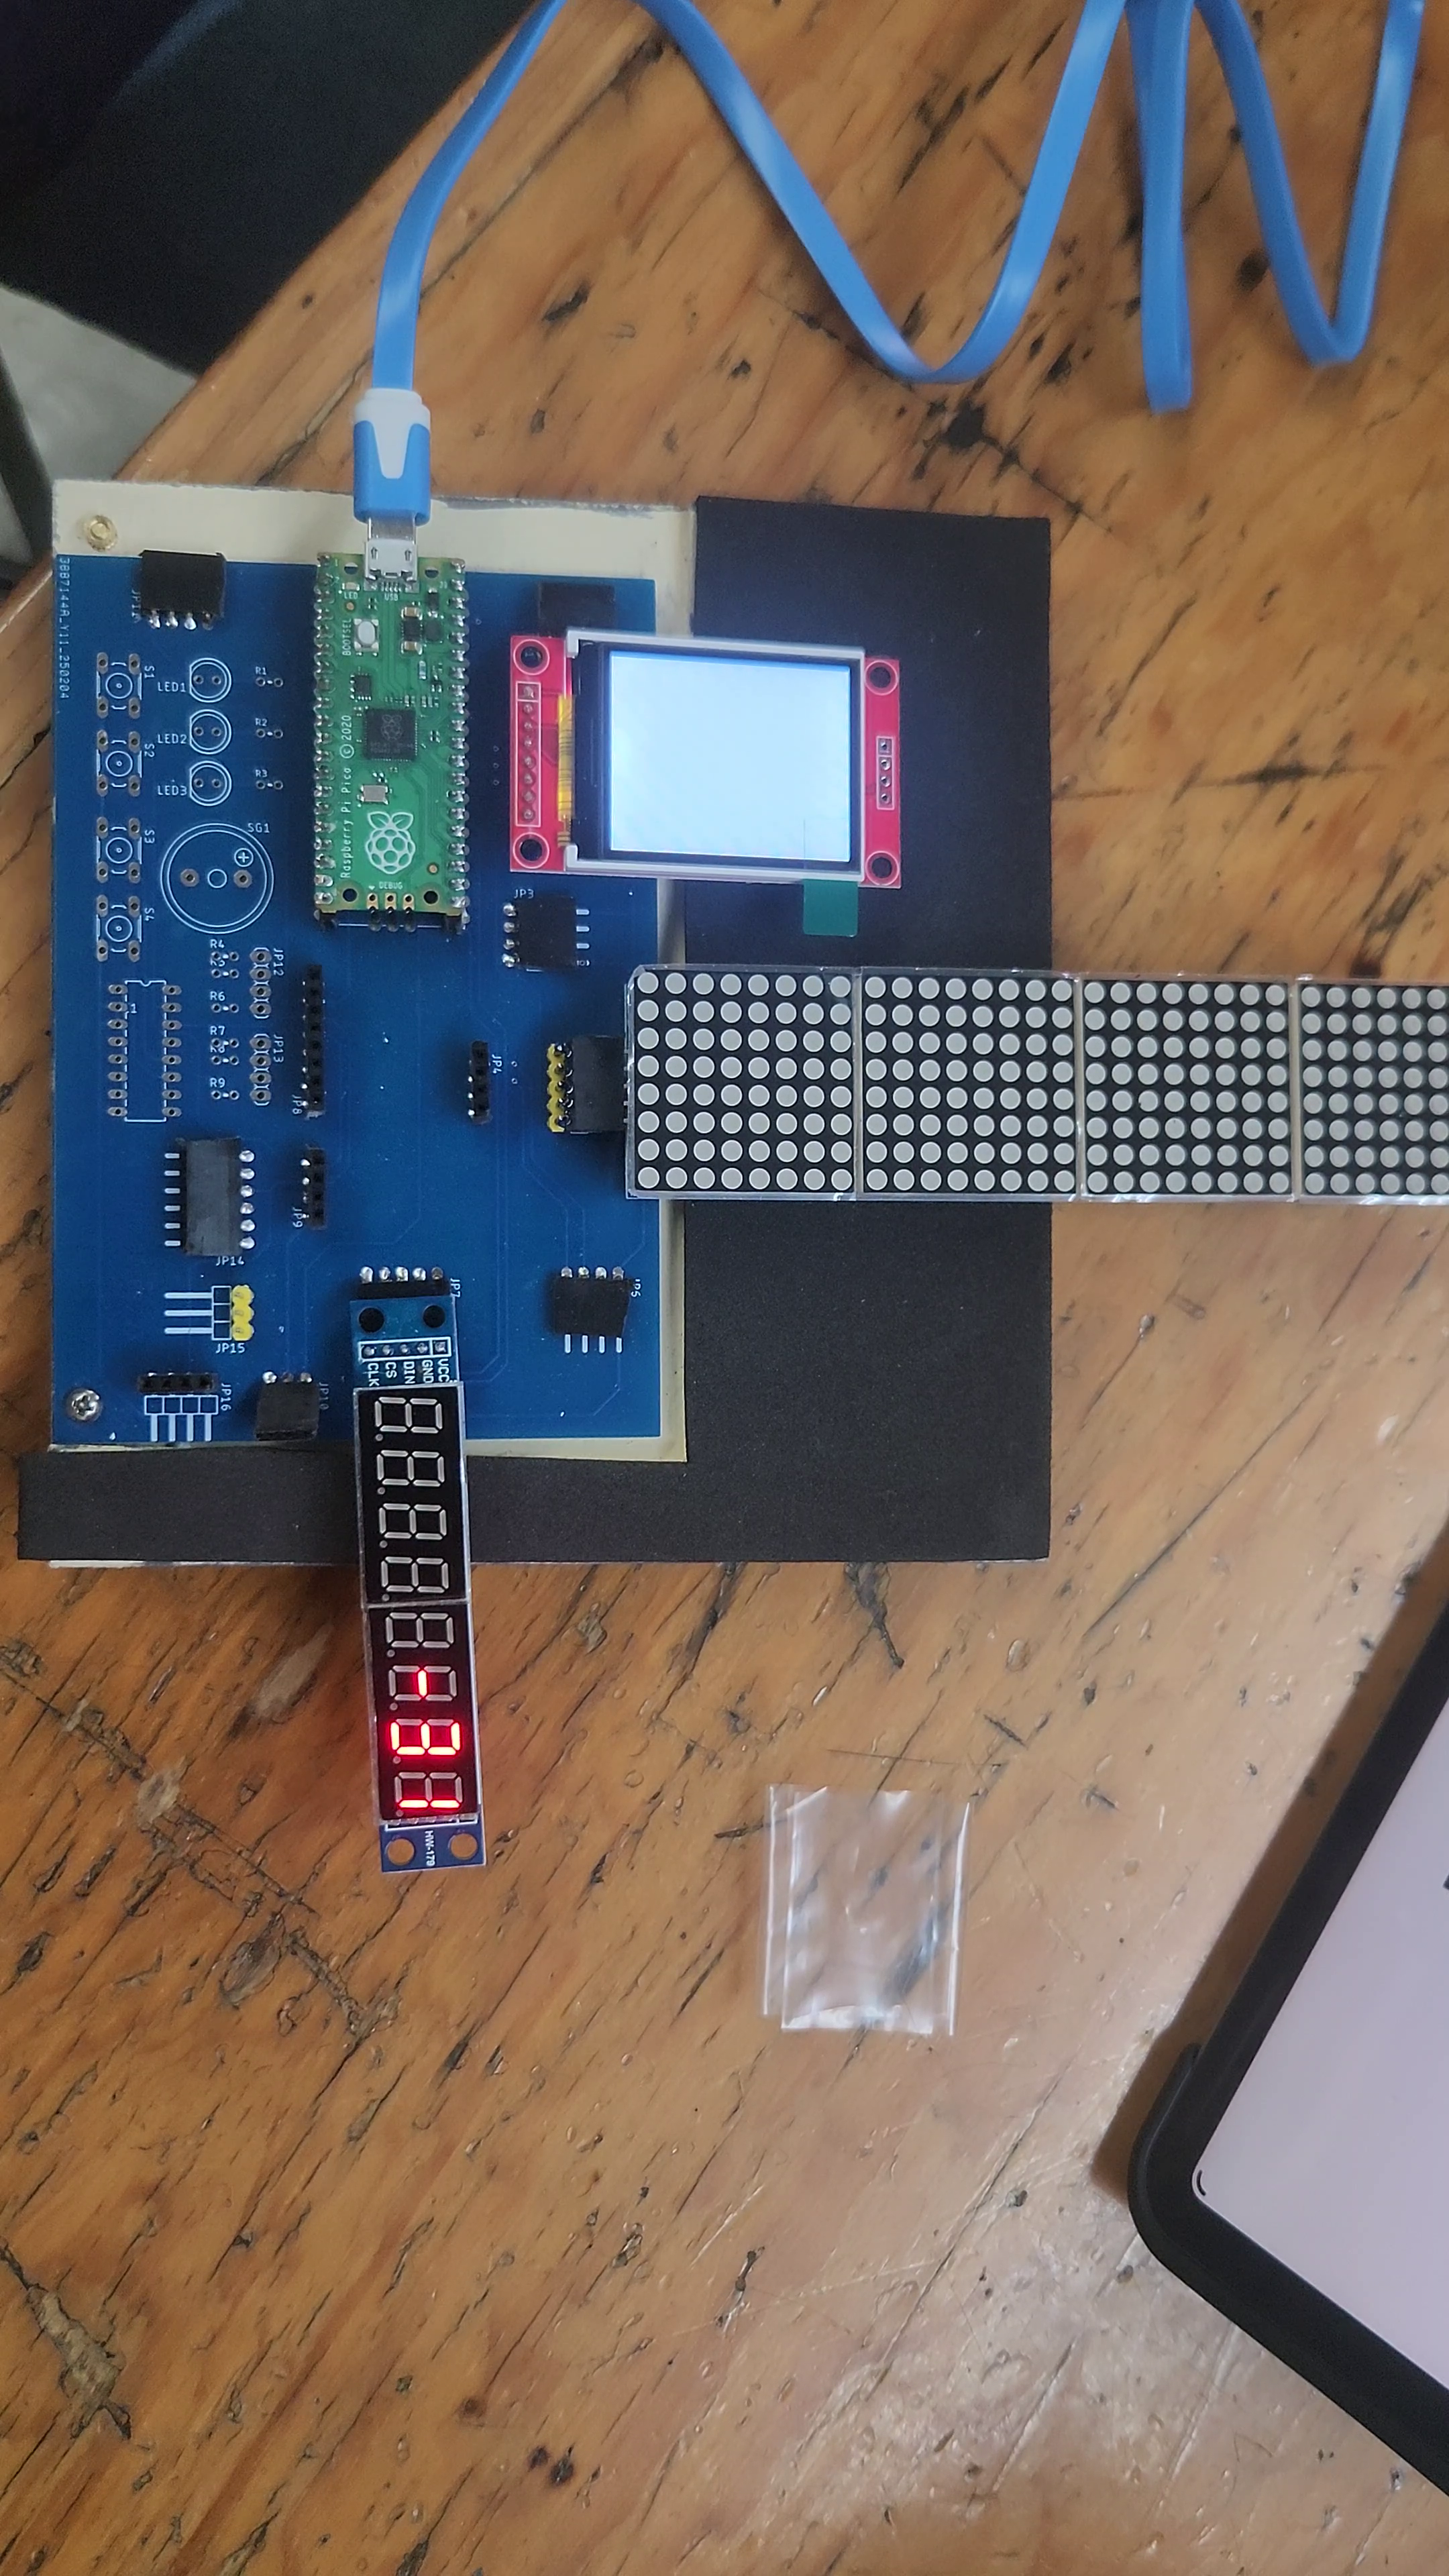
\includegraphics[width=0.55\linewidth, angle=90]{img/Actividad2/Act2_13.png}
            \caption{Actividad 2 - Contador Descendente: \texttt{-31}}
        \end{subfigure}
        \caption{Actividad 2 - Contador Descendente.}
    \end{figure}

    \subsection*{Análisis de resultados}

    A partir de las imágenes obtenidas durante la ejecución del programa, se puede observar que el contador ascendente inicia en \texttt{138} y va incrementando de uno en uno cada medio segundo, hasta llegar a \texttt{143} de forma que el incremento se realiza de manera correcta y su visualización en el display es la esperada. De igual forma, el contador descendente inicia en \texttt{-26} y va decrementando de uno en uno cada medio segundo, hasta llegar a \texttt{-31} de forma que el decremento se realiza de manera correcta y su visualización en el display es la esperada. Por lo que la comunicación SPI con el display se encuentra funcionando correctamente, y el programa cumple con los requisitos establecidos en la tabla de la actividad. 

    \newpage
    \section*{Actividad 3}

\begin{tikzpicture}

    % Texto de la Actividad 3
    \node[text width=15.5cm, align=justify, font=\sffamily] at (-2.5, 3) {
        Escribir el siguiente programa, cerciorarse que el módulo Matriz MAX7219 de 4 elementos matriciales de 8x8, se encuentre conectado en la posición correcta; investigar el funcionamiento de la librería max7219.py; comentar el código.
    };

    % Llamada a la Raspberry Pi Pico
    \picoboard

    % ==========================================
    % MÓDULO MATRIZ 8x8x4 Y CONEXIONES
    % ==========================================

    % Título de la Matriz
    \node[above right, text=blue!60!black, font=\itshape\sffamily] at (-9.3, -0.9) {Matriz 8x8 x 4};

    % Contorno del Módulo
    \draw[thick] (-9.5, -1.0) rectangle (-2.0, -3.5);

    % Las 4 matrices de 8x8
    \foreach \i in {0,...,3} {
        \draw[thick] (-9.2 + \i*1.4, -1.3) rectangle ++(1.2, -1.9);
    }

    % Etiquetas de los pines
    \node[left, font=\small\sffamily\bfseries] at (-2.1, -1.35) {VCC};
    \node[left, font=\small\sffamily\bfseries] at (-2.1, -1.8) {CLK};
    \node[left, font=\small\sffamily\bfseries] at (-2.1, -2.25) {MOSI};
    \node[left, font=\small\sffamily\bfseries] at (-2.1, -3.15) {CS};

    % --- CONEXIONES A LA PICO ---
    
    % Conexión CLK (Azul) a GP2
    \draw[blue, thick] (-2.0, -1.8) -- (P4);
    
    % Conexión MOSI (Verde) a GP3
    \draw[green!60!black, thick] (-2.0, -2.25) -- (P5);
    
    % Conexión CS (Roja) a GP6
    \draw[red, thick] (-2.0, -3.15) -- (P9);

    % --- CONEXIONES DE ENERGÍA ---

    % Conexión VCC y VBUS
    \draw[red, thick] (-2.5, -1.0) -- (-2.5, -0.3) -- (-1.8, -0.3) node[right, font=\small\sffamily\bfseries, text=black] {\textbf{VBUS}};
    \node[above, font=\small\sffamily\bfseries] at (-2.5, -0.3) {5V};

    % Conexión GND
    \draw[thick] (-3.0, -3.5) -- (-3.0, -4.5);
    
    % Símbolo de Tierra (GND)
    \draw[thick] (-3.4, -4.5) -- (-2.6, -4.5);
    \draw[thick] (-3.2, -4.65) -- (-2.8, -4.65);
    \draw[thick] (-3.05, -4.8) -- (-2.95, -4.8);
    \node[right, font=\small\sffamily\bfseries] at (-2.6, -4.65) {GND};

\end{tikzpicture}

\newpage
\textbf{Código}

\lstinputlisting[language={[LAB]Python}, caption={Código de la Actividad 3 - Matriz MAX7219 de 4x8x8}, basicstyle=\ttfamily\scriptsize]{Code/Act3b.py}

\subsection*{Propuesta de solución}

El siguiente código configura una matriz de LEDs de 4 módulos de 8x8 píxeles controlada por el chip MAX7219 mediante comunicación SPI. Se inicializa el bus SPI0 con los pines GPIO2 (reloj) y GPIO3 (datos), y se utiliza el pin GPIO6 como selección de chip (CS). Se define la variable \texttt{num\_display = 4} para indicar la cantidad de módulos conectados en cascada. El programa limpia la pantalla, dibuja el carácter "0" en la coordenada (0,1) y lo muestra durante 3 segundos.

\begin{center}
\begin{tikzpicture}[
    node distance=6mm and 12mm,
    every node/.style={font=\footnotesize\sffamily}
]
    \node (inicio) [startstop] {Inicio};
    \node (import) [process, below=of inicio, text width=5.5cm, align=center] {Importar librerías:\\ \texttt{max7219, Pin, SPI, sleep}};
    \node (num) [process, below=of import, text width=5.5cm, align=center] {Definir \texttt{num\_display = 4}\\ (módulos en cascada)};
    \node (spi) [process, below=of num, text width=5.5cm, align=center] {Configurar \texttt{SPI(0)}\\ con SCK=GP2, MOSI=GP3\\ frecuencia=10 MHz};
    \node (cs) [process, below=of spi, text width=5.5cm, align=center] {Configurar \texttt{CS=GP6}\\ como salida digital};
    \node (matrix) [process, below=of cs, text width=5.5cm, align=center] {Crear objeto \texttt{display}\\ de la clase \texttt{Matrix8x8}};
    \node (fill) [process, below=of matrix, text width=5.5cm, align=center] {Limpiar pantalla\\ con \texttt{display.fill(0)}};
    \node (text) [process, below=of fill, text width=5.5cm, align=center] {Dibujar \texttt{'0'} en (0,1)\\ con \texttt{display.text()}};
    \node (show) [process, below=of text, text width=5.5cm, align=center] {Actualizar pantalla\\ con \texttt{display.show()}};
    \node (sleep) [process, below=of show, text width=5.5cm, align=center] {Esperar 3 segundos\\ con \texttt{sleep(3)}};
    \node (fin) [startstop, below=of sleep] {Fin};

    \draw [arrow] (inicio) -- (import);
    \draw [arrow] (import) -- (num);
    \draw [arrow] (num) -- (spi);
    \draw [arrow] (spi) -- (cs);
    \draw [arrow] (cs) -- (matrix);
    \draw [arrow] (matrix) -- (fill);
    \draw [arrow] (fill) -- (text);
    \draw [arrow] (text) -- (show);
    \draw [arrow] (show) -- (sleep);
    \draw [arrow] (sleep) -- (fin);
\end{tikzpicture}
\end{center}

\subsection*{Investigación: Librería \texttt{max7219.py}}

La librería \texttt{max7219.py} es un controlador escrito en MicroPython diseñado específicamente para manejar módulos de matrices de LEDs de 8x8 píxeles basados en el chip MAX7219. Esta librería es fundamental cuando se trabaja con displays gráficos matriciales, a diferencia de la librería \texttt{max7219\_8digit} que se usa para displays de 7 segmentos.

\textbf{Principales características y funciones:}

\begin{itemize}
    \item \textbf{Soporte para múltiples módulos en cascada:} El parámetro \texttt{num\_display} permite indicar cuántos módulos de 8x8 están conectados en serie, extendiendo el ancho total de la pantalla (por ejemplo, 4 módulos generan una resolución de 32x8 píxeles).
    
    \item \textbf{Método \texttt{fill(value)}:} Permite limpiar o llenar completamente la pantalla. Con \texttt{fill(0)} se apagan todos los LEDs, mientras que \texttt{fill(1)} los enciende todos.
    
    \item \textbf{Método \texttt{text(string, x, y, color)}:} Dibuja un carácter o cadena de texto en las coordenadas especificadas. El parámetro \texttt{color} puede ser 1 (LED encendido) o 0 (LED apagado). La librería incluye una matriz de píxeles para cada carácter de la fuente predeterminada.
    
    \item \textbf{Método \texttt{show()}:} Una vez que se han realizado todas las modificaciones en el buffer interno (con \texttt{fill}, \texttt{text}, \texttt{pixel}, etc.), esta función envía los datos al hardware para actualizar la pantalla físicamente.
    
    \item \textbf{Método \texttt{pixel(x, y, color)}:} Permite controlar un LED individual en la posición (x, y) de la matriz.
\end{itemize}

En resumen, esta librería abstrae la complejidad del protocolo de comunicación con el MAX7219 y proporciona una interfaz sencilla tipo framebuffer para dibujar texto y gráficos en matrices de LEDs.

\subsection*{Desarrollo}

\textbf{Código comentado}

\lstinputlisting[language={[LAB]Python}, caption={Código de la Actividad 3 - Matriz MAX7219 de 4x8x8}, basicstyle=\ttfamily\scriptsize]{Code/Act3.py}

\begin{figure}[H]
    \centering
        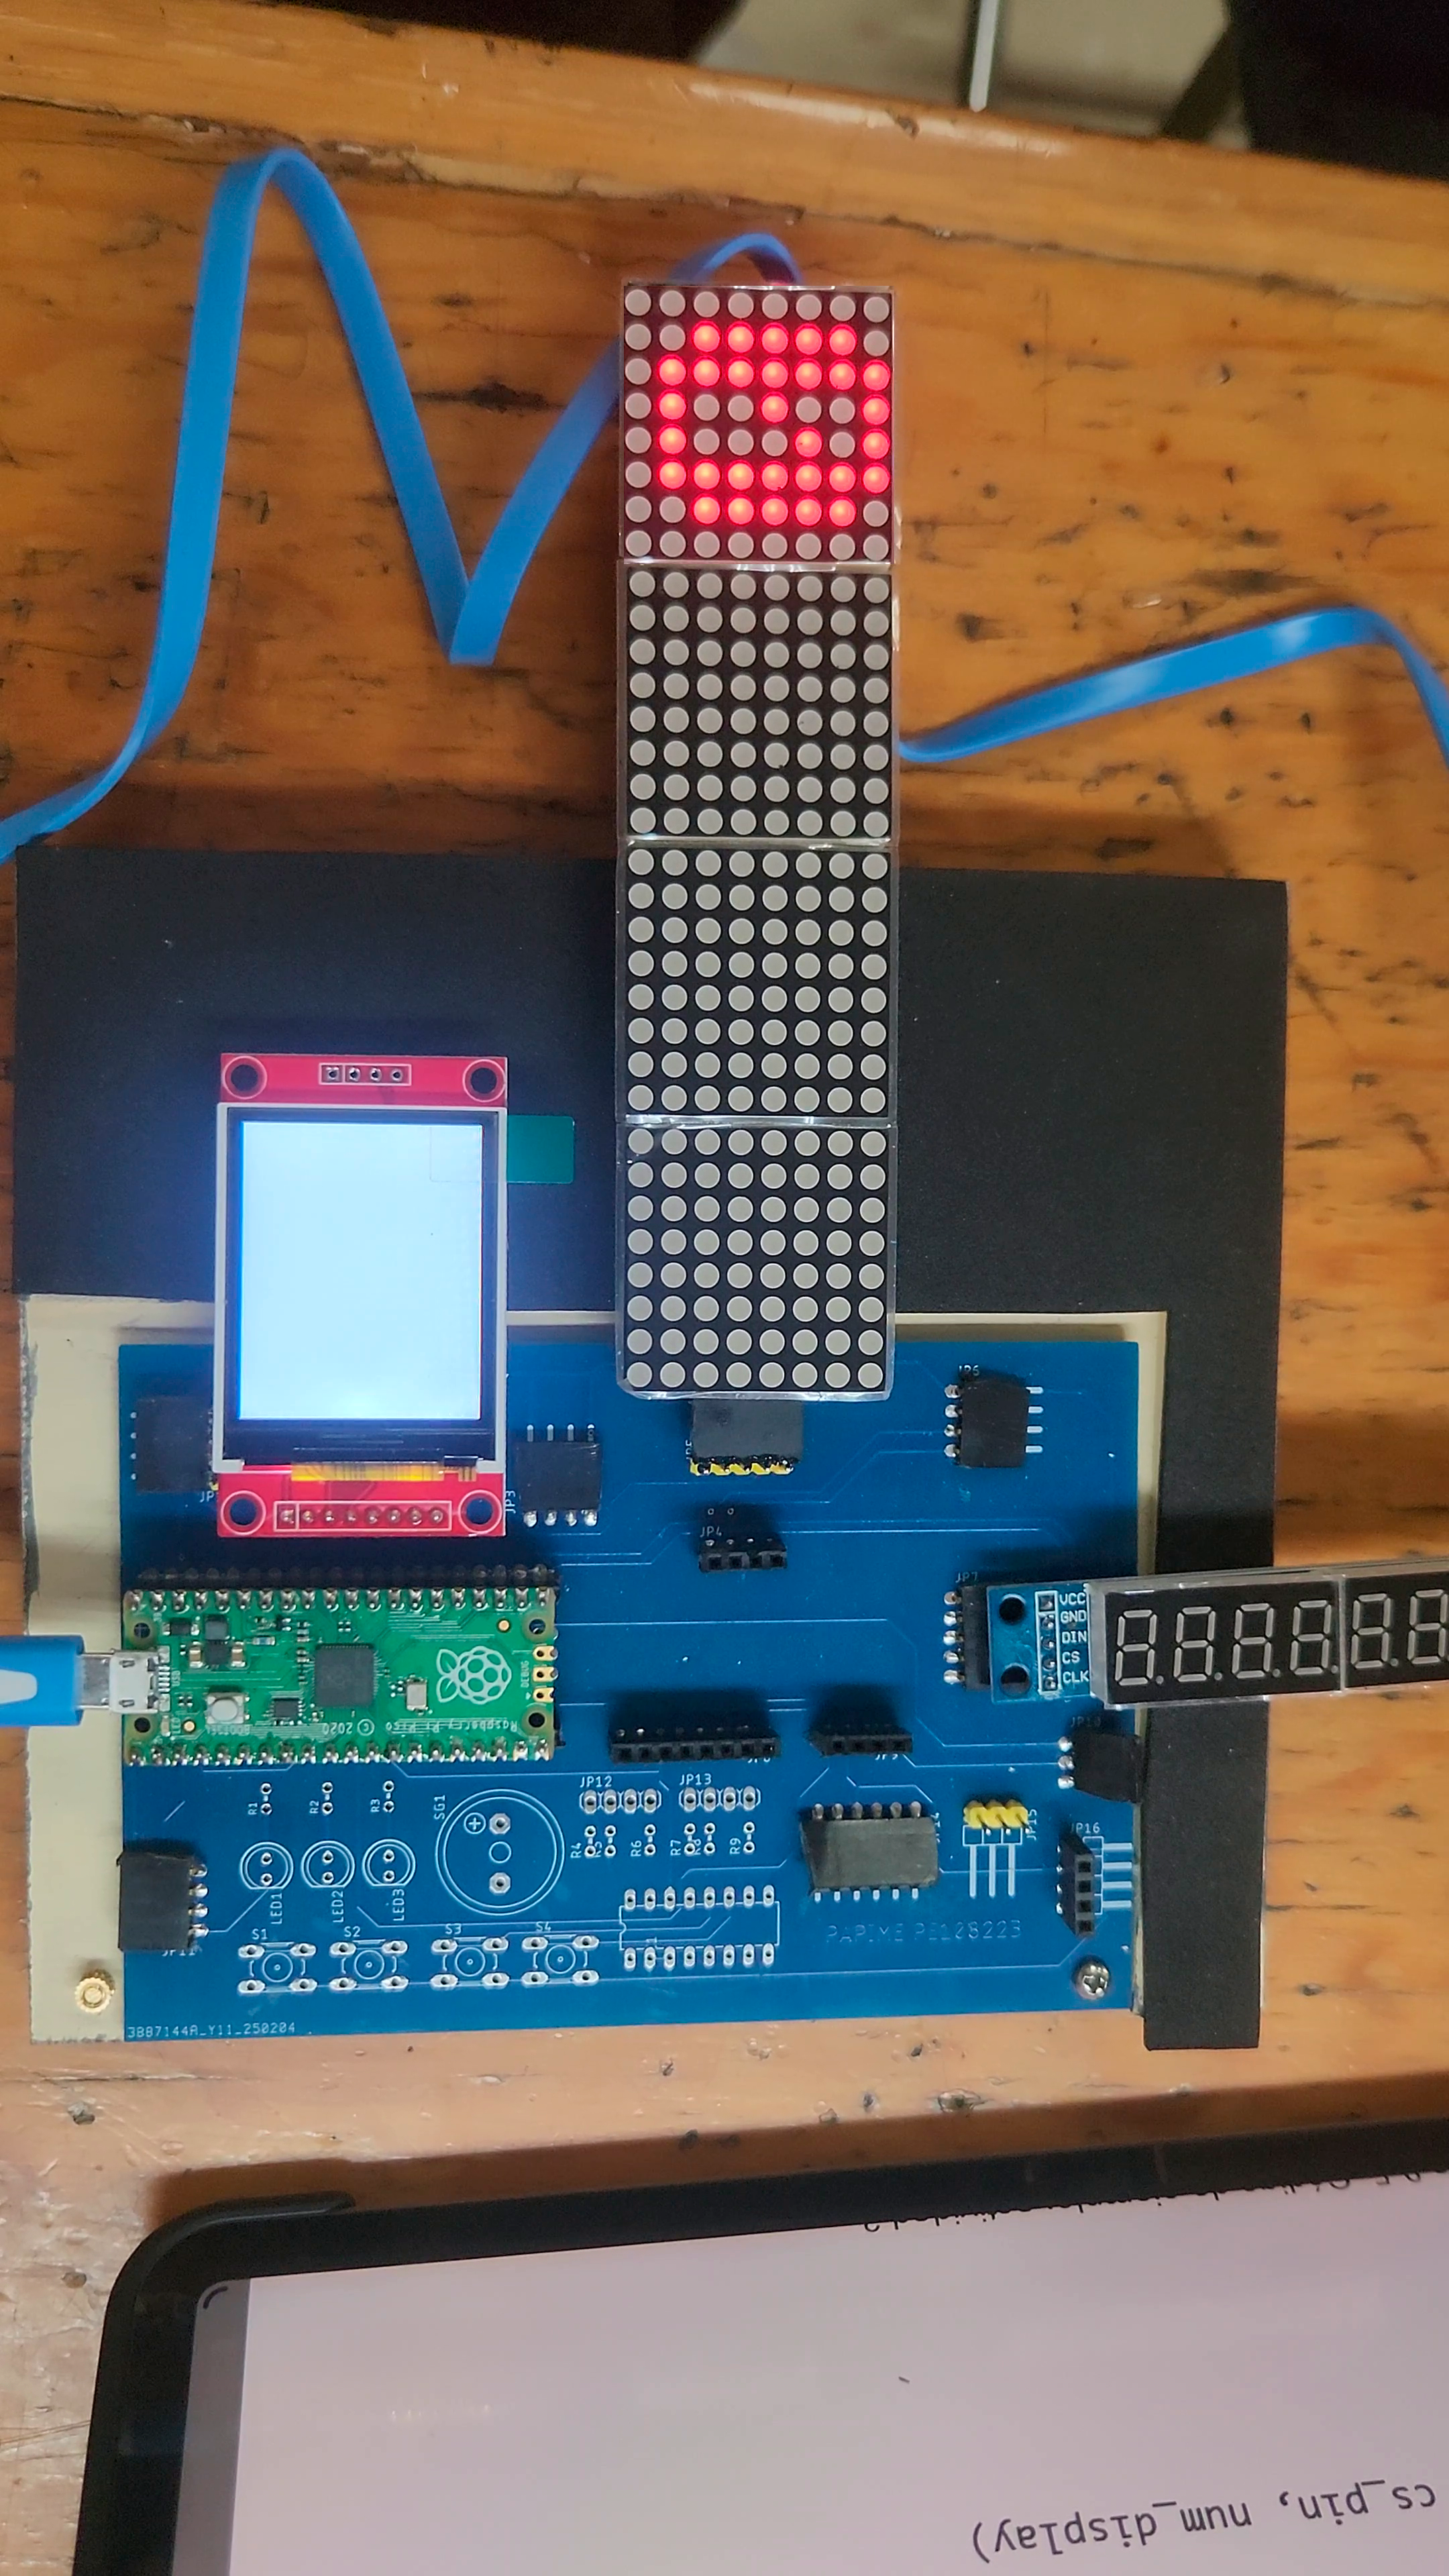
\includegraphics[width=0.4\textwidth, angle=90]{img/Actividad3/Act3_1.png}
        \caption{Visualización del carácter "0" en la posición (0,1).}
\end{figure}

\subsection*{Análisis de resultados}

La ejecución del código logró mostrar correctamente el carácter "0" en la matriz de LEDs de 4 módulos 8x8. La configuración del bus SPI con una frecuencia de 10 MHz fue adecuada para la comunicación con el MAX7219, y el uso del pin GPIO6 como Chip Select permitió seleccionar correctamente el dispositivo. La librería \texttt{max7219.py} facilitó el control de la matriz, permitiendo limpiar la pantalla con \texttt{fill(0)} y dibujar texto con coordenadas específicas mediante \texttt{text()} y se verificó que la función \texttt{show()} es esencial para transferir los datos del buffer interno al hardware.

\newpage 

    \section*{Actividad 4}

    Usando la matriz de leds SPI, desplegar los siguientes mensajes, usar intervalos de
    tiempo de 2 segundos entre cada uno de ellos (puede ser texto fijo o con desplazamiento).

    \begin{center}
        \sffamily\Large\bfseries
        \setlength{\tabcolsep}{8pt} % Espaciado entre columnas
        \renewcommand{\arraystretch}{1.3} % Espaciado entre filas
        
        \begin{tabular}{cccc l}
        \textcolor{blue!60!black}{U} & \textcolor{blue!60!black}{N} & \textcolor{blue!60!black}{A} & \textcolor{blue!60!black}{M} & \\
        \textcolor{cyan!80!blue}{*} & \textcolor{cyan!80!blue}{F} & \textcolor{cyan!80!blue}{I} & \textcolor{cyan!80!blue}{*} & \\
        \textcolor{blue!60!black}{2} & \textcolor{blue!60!black}{0} & \textcolor{blue!60!black}{2} & \textcolor{blue!60!black}{5} & \\
        \textcolor{cyan!80!blue}{2} & \textcolor{cyan!80!blue}{5} & \textcolor{cyan!80!blue}{-} & \textcolor{cyan!80!blue}{2} & \\
        \textcolor{blue!60!black}{*} & \textcolor{blue!60!black}{*} & \textcolor{blue!60!black}{*} & \textcolor{blue!60!black}{*} & \hspace{0.5cm} {\mdseries\upshape\textit{- Texto libre}} \\
        \end{tabular}
        
        \vspace{15pt}
        \normalsize\normalfont\sffamily Figura 8-6. Actividad 4
    \end{center}

    \subsection*{Propuesta de solución}
    Para mostrar los textos en las matrices de LEDs, se configura el bus SPI del microcontrolador RP2040 para comunicarse con el controlador MAX7219. Este circuito integrado maneja las cuatro matrices de 8x8 conectadas en cascada. Se definen los pines de reloj (SCK), salida de datos maestros (MOSI) y selección de chip (CS). 
    
    En el código, se crea una lista que almacena exactamente las cadenas de texto solicitadas por el manual ("UNAM", "FI", "*", "2026", "26 - 2", "PEPE"). La solución implementa un bucle \texttt{for} infinito que recorre esta lista elemento por elemento. En cada paso, el programa limpia la memoria de la pantalla para evitar que los textos se encimen, dibuja los caracteres arrancando desde la coordenada inicial de la matriz y aplica un retardo de 2 segundos mediante \texttt{sleep(2)} para que cada mensaje permanezca visible el tiempo requerido antes de pasar al siguiente.

    \begin{center}
        \begin{tikzpicture}[
            node distance=8mm and 14mm,
            every node/.style={font=\small\sffamily}
        ]
            % --- Nodos ---
            \node (inicio) [startstop] {Inicio};
            \node (spi) [process, below=of inicio, text width=6.0cm, align=center] {Configurar \texttt{SPI(0)}\\ y crear la matriz \texttt{MAX7219}};
            \node (lista) [process, below=of spi, text width=6.0cm, align=center] {Definir la lista de mensajes\\ \texttt{"UNAM", "FI", "*", "*", "2026", "26 - 2", "*", "*", "*", "*", "PEPE"}};
            \node (bucle) [process, below=of lista, text width=5.6cm, align=center] {Entrar al ciclo infinito\\ \texttt{while True}};
            \node (mensaje) [decision, below=of bucle, text width=4.2cm, align=center] {¿Queda un mensaje\\ por mostrar?};
            \node (limpia) [process, right=18mm of mensaje, text width=4.6cm, align=center] {Limpiar la pantalla\\ con \texttt{fill(0)}};
            \node (escribe) [process, below=of limpia, text width=4.6cm, align=center] {Escribir el mensaje\\ en \texttt{(0,0)}};
            \node (muestra) [process, below=of escribe, text width=4.6cm, align=center] {Actualizar el display\\ con \texttt{show()}};
            \node (espera) [process, below=of muestra, text width=4.6cm, align=center] {Esperar 2 segundos\\ con \texttt{sleep(2)}};

            % --- Conexiones Lineales ---
            \draw [arrow] (inicio) -- (spi);
            \draw [arrow] (spi) -- (lista);
            \draw [arrow] (lista) -- (bucle);
            \draw [arrow] (bucle) -- (mensaje);


            \draw [arrow] (mensaje.east) -- node[above, font=\scriptsize]{Sí} (limpia.west);
            
            \draw [arrow] (limpia) -- (escribe);
            \draw [arrow] (escribe) -- (muestra);
            \draw [arrow] (muestra) -- (espera);


            \draw [arrow] (espera.south) -- ++(0,-0.8) -| (mensaje.south);


            \draw [arrow] (mensaje.west) -- node[above, pos=0.2, font=\scriptsize]{No} ++(-1.5,0) |- (bucle.west);

        \end{tikzpicture}
    \end{center}

    \noindent El flujo de datos recorre la lista \texttt{mensajes} de forma secuencial: cada cadena se limpia, se convierte en puntos encendidos dentro del framebuffer del MAX7219 y se envía al módulo por SPI antes de pausar dos segundos. Al terminar la lista, el ciclo \texttt{while True} vuelve a comenzar y vuelve a recorrer los mensajes sin detener la ejecución.

    \subsection*{Desarrollo}

    \lstinputlisting[language={[LAB]Python}, caption={Código de la Actividad 4 - Comunicación UART}, basicstyle=\ttfamily\scriptsize]{Code/Act4.py}

    \begin{figure}[H]
        \centering
        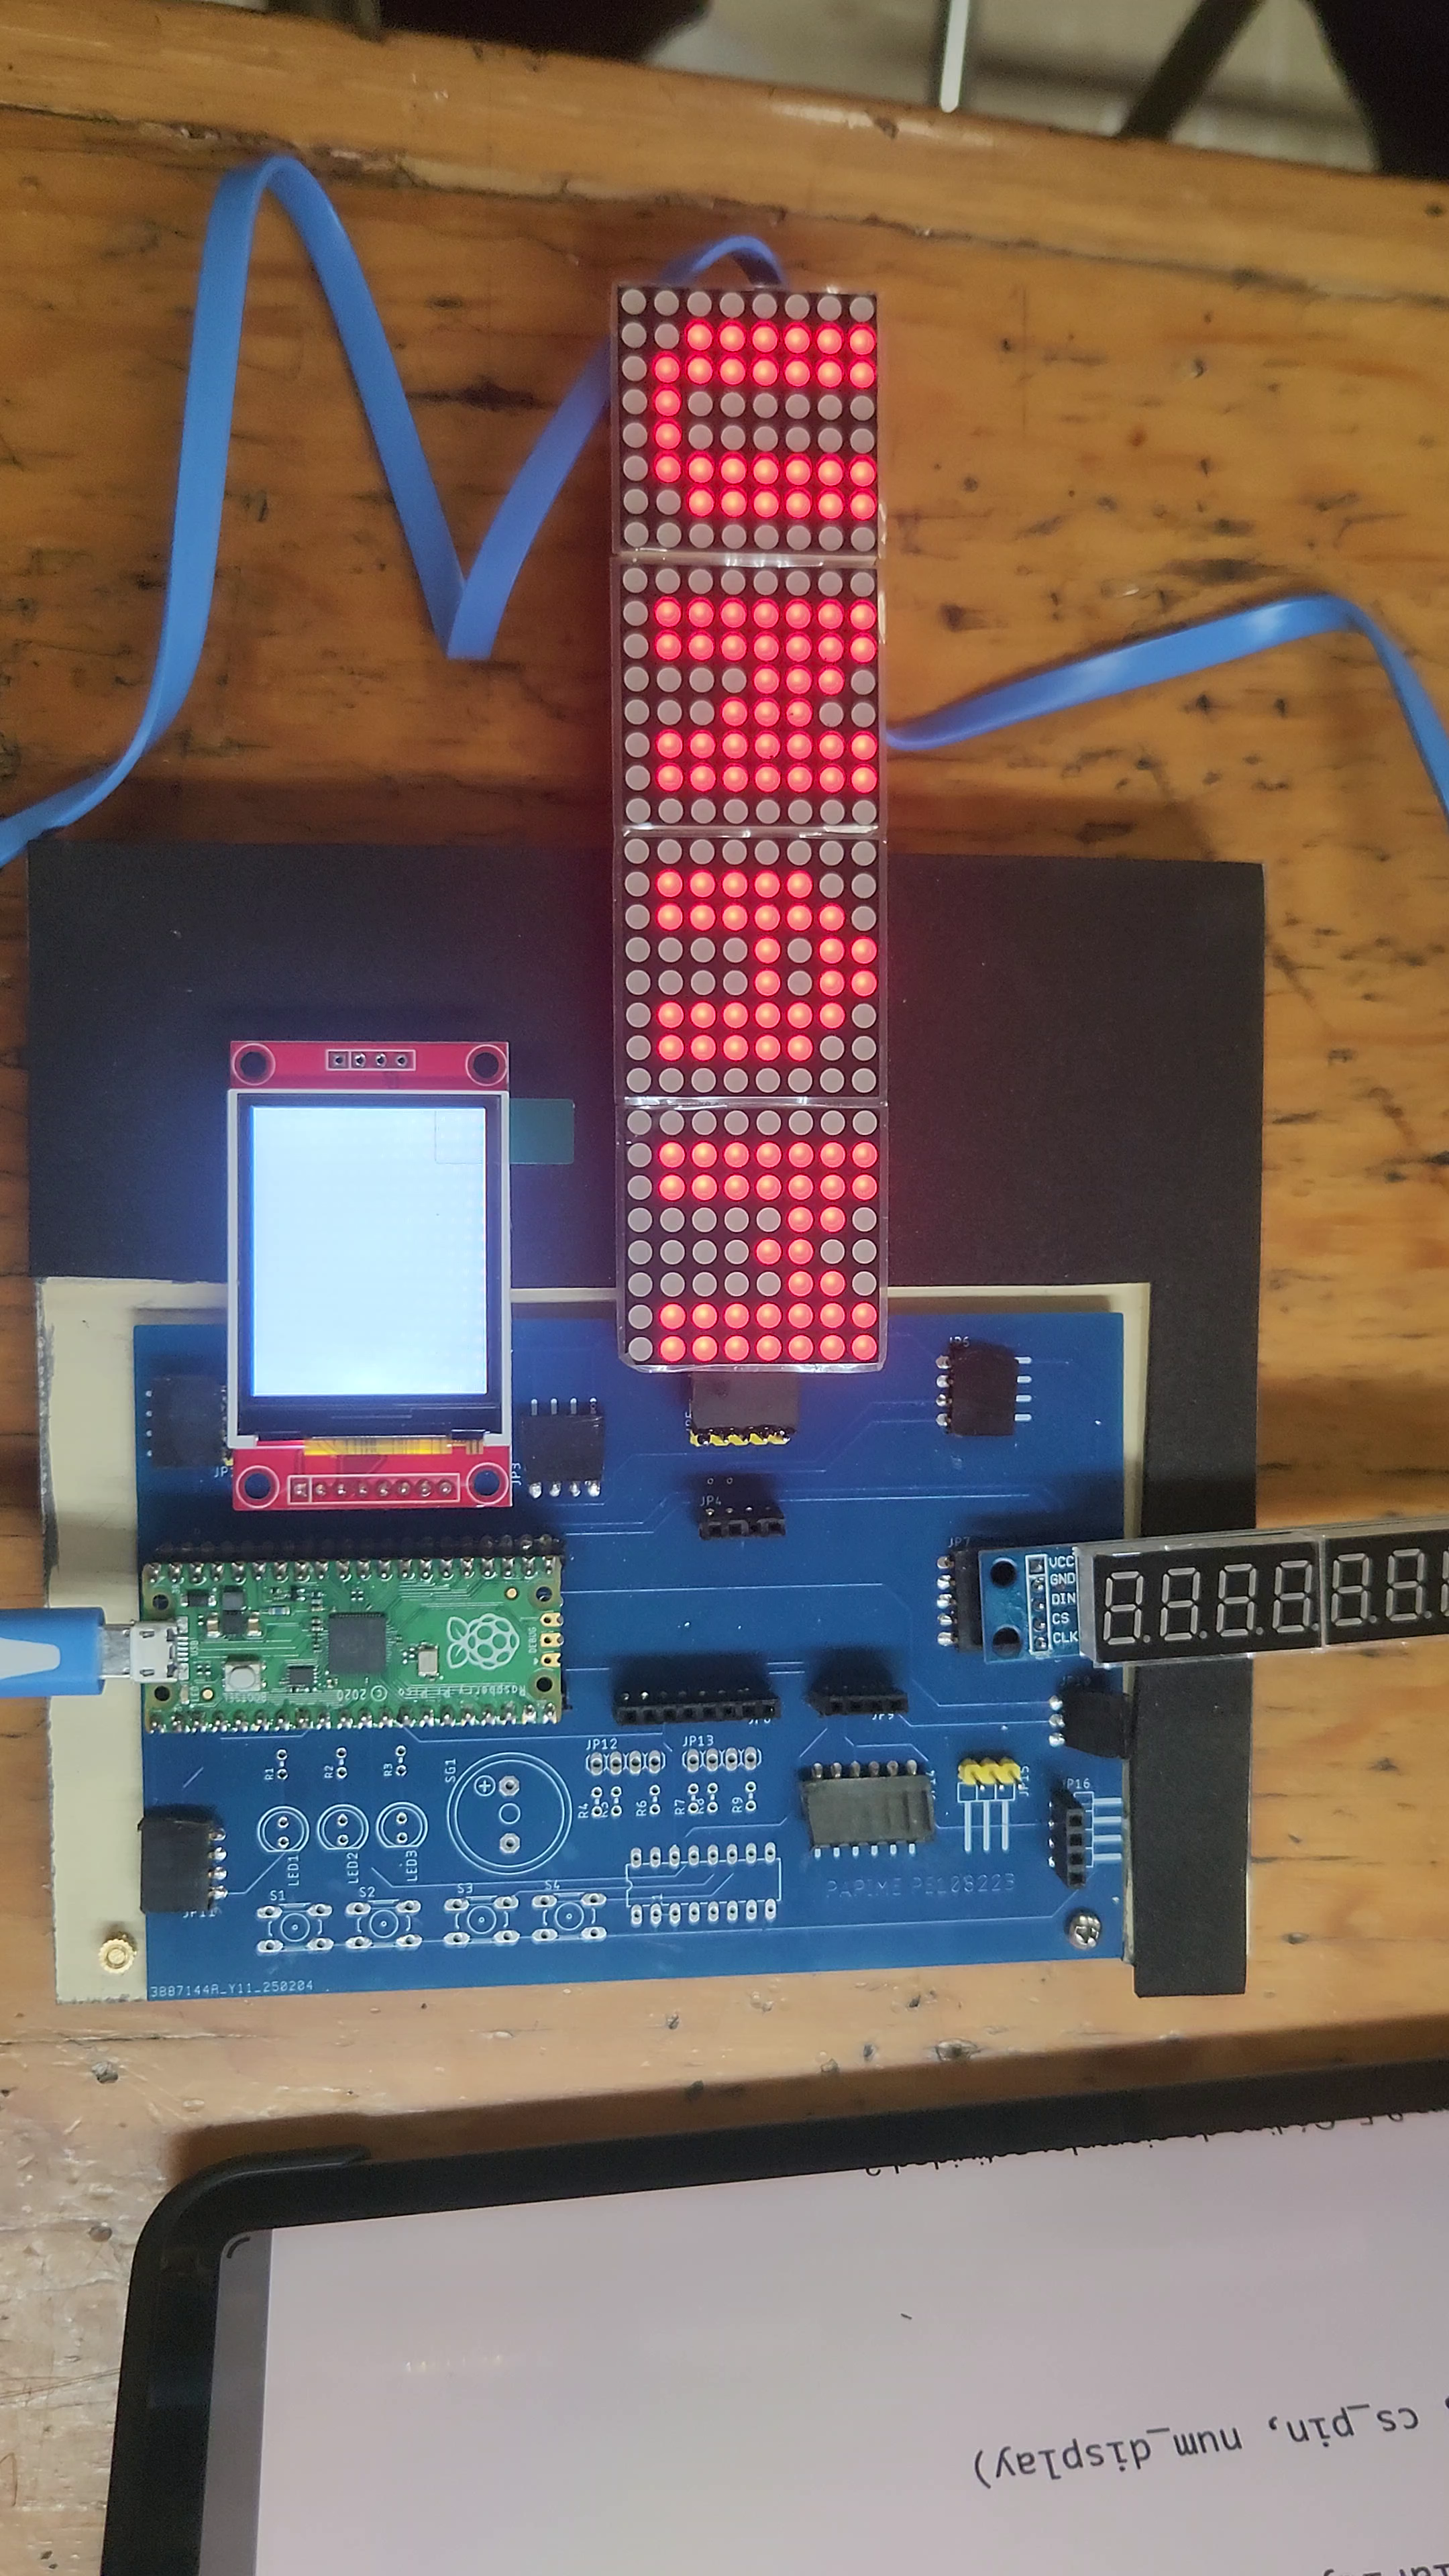
\includegraphics[width=0.5\textwidth, angle=90]{img/Actividad4/Act4_8.png}
        \caption{Texto UNAM.}
    \end{figure}
    \begin{figure}[H]
        \centering
        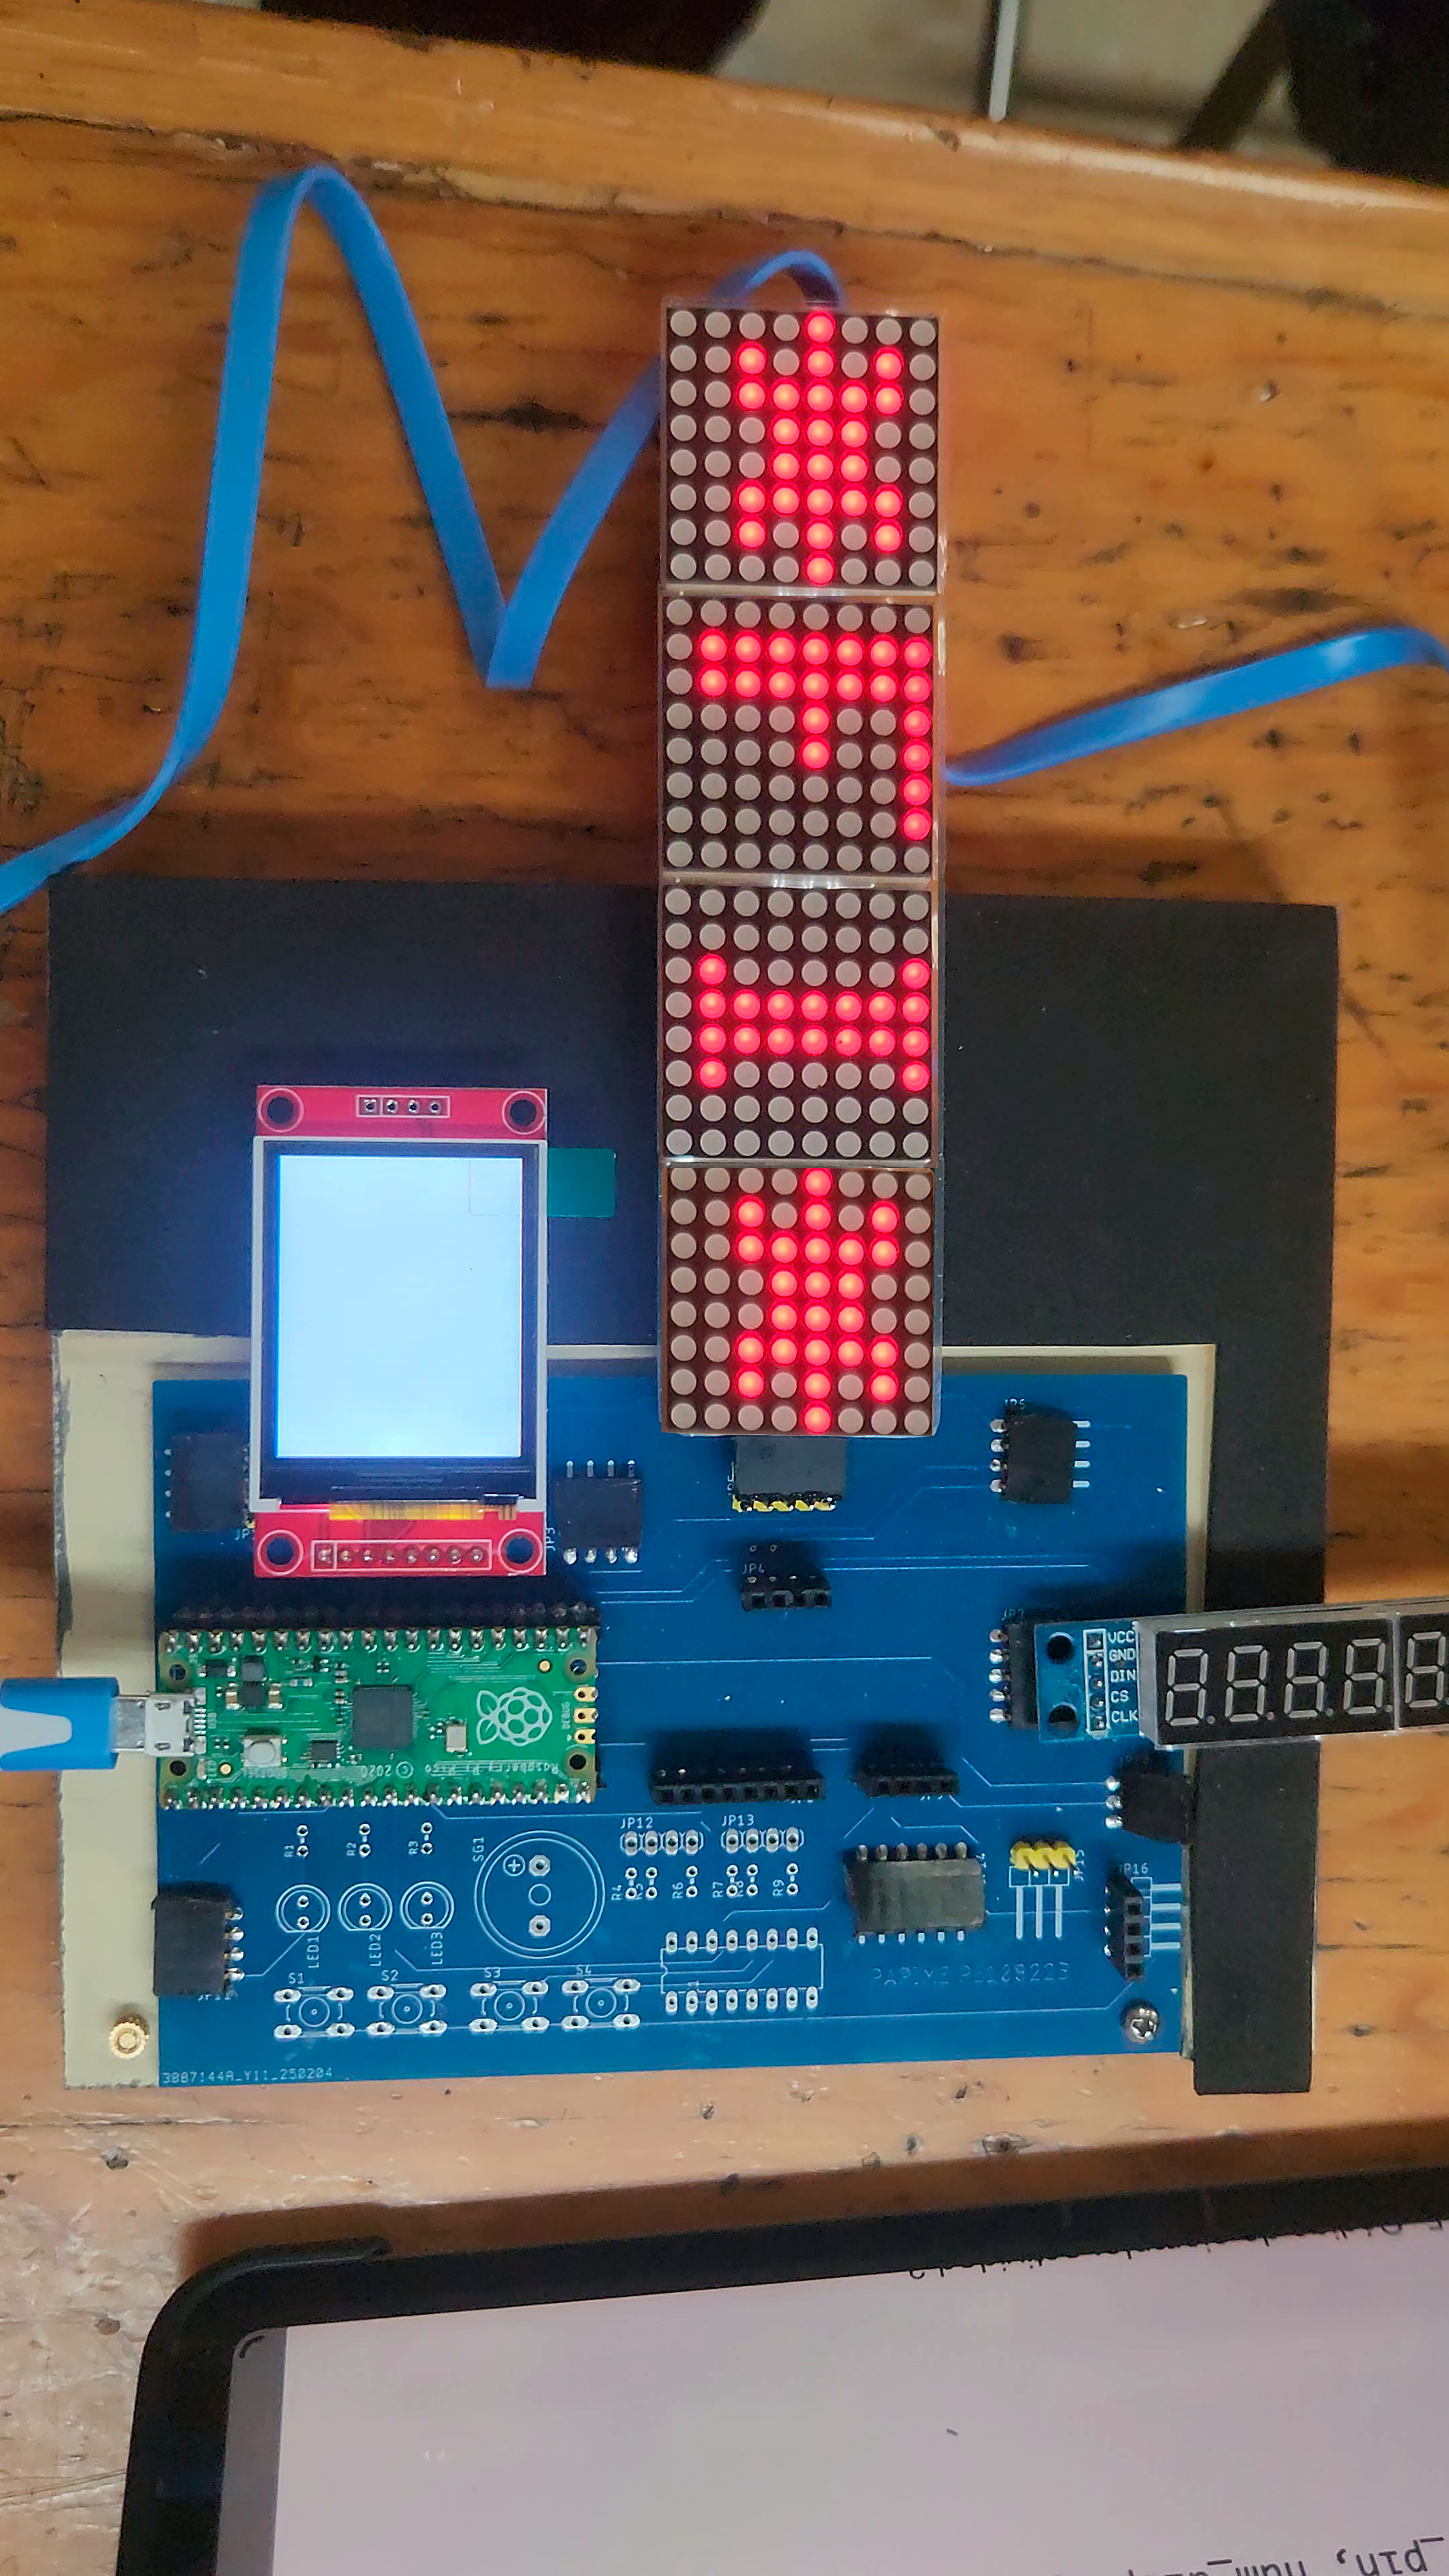
\includegraphics[width=0.5\textwidth, angle=90]{img/Actividad4/Act4_1.png}
        \caption{El microcontrolador transfiere la cadena "FI" mediante la línea MOSI del bus SPI.}
    \end{figure}

    \begin{figure}[H]
        \centering
        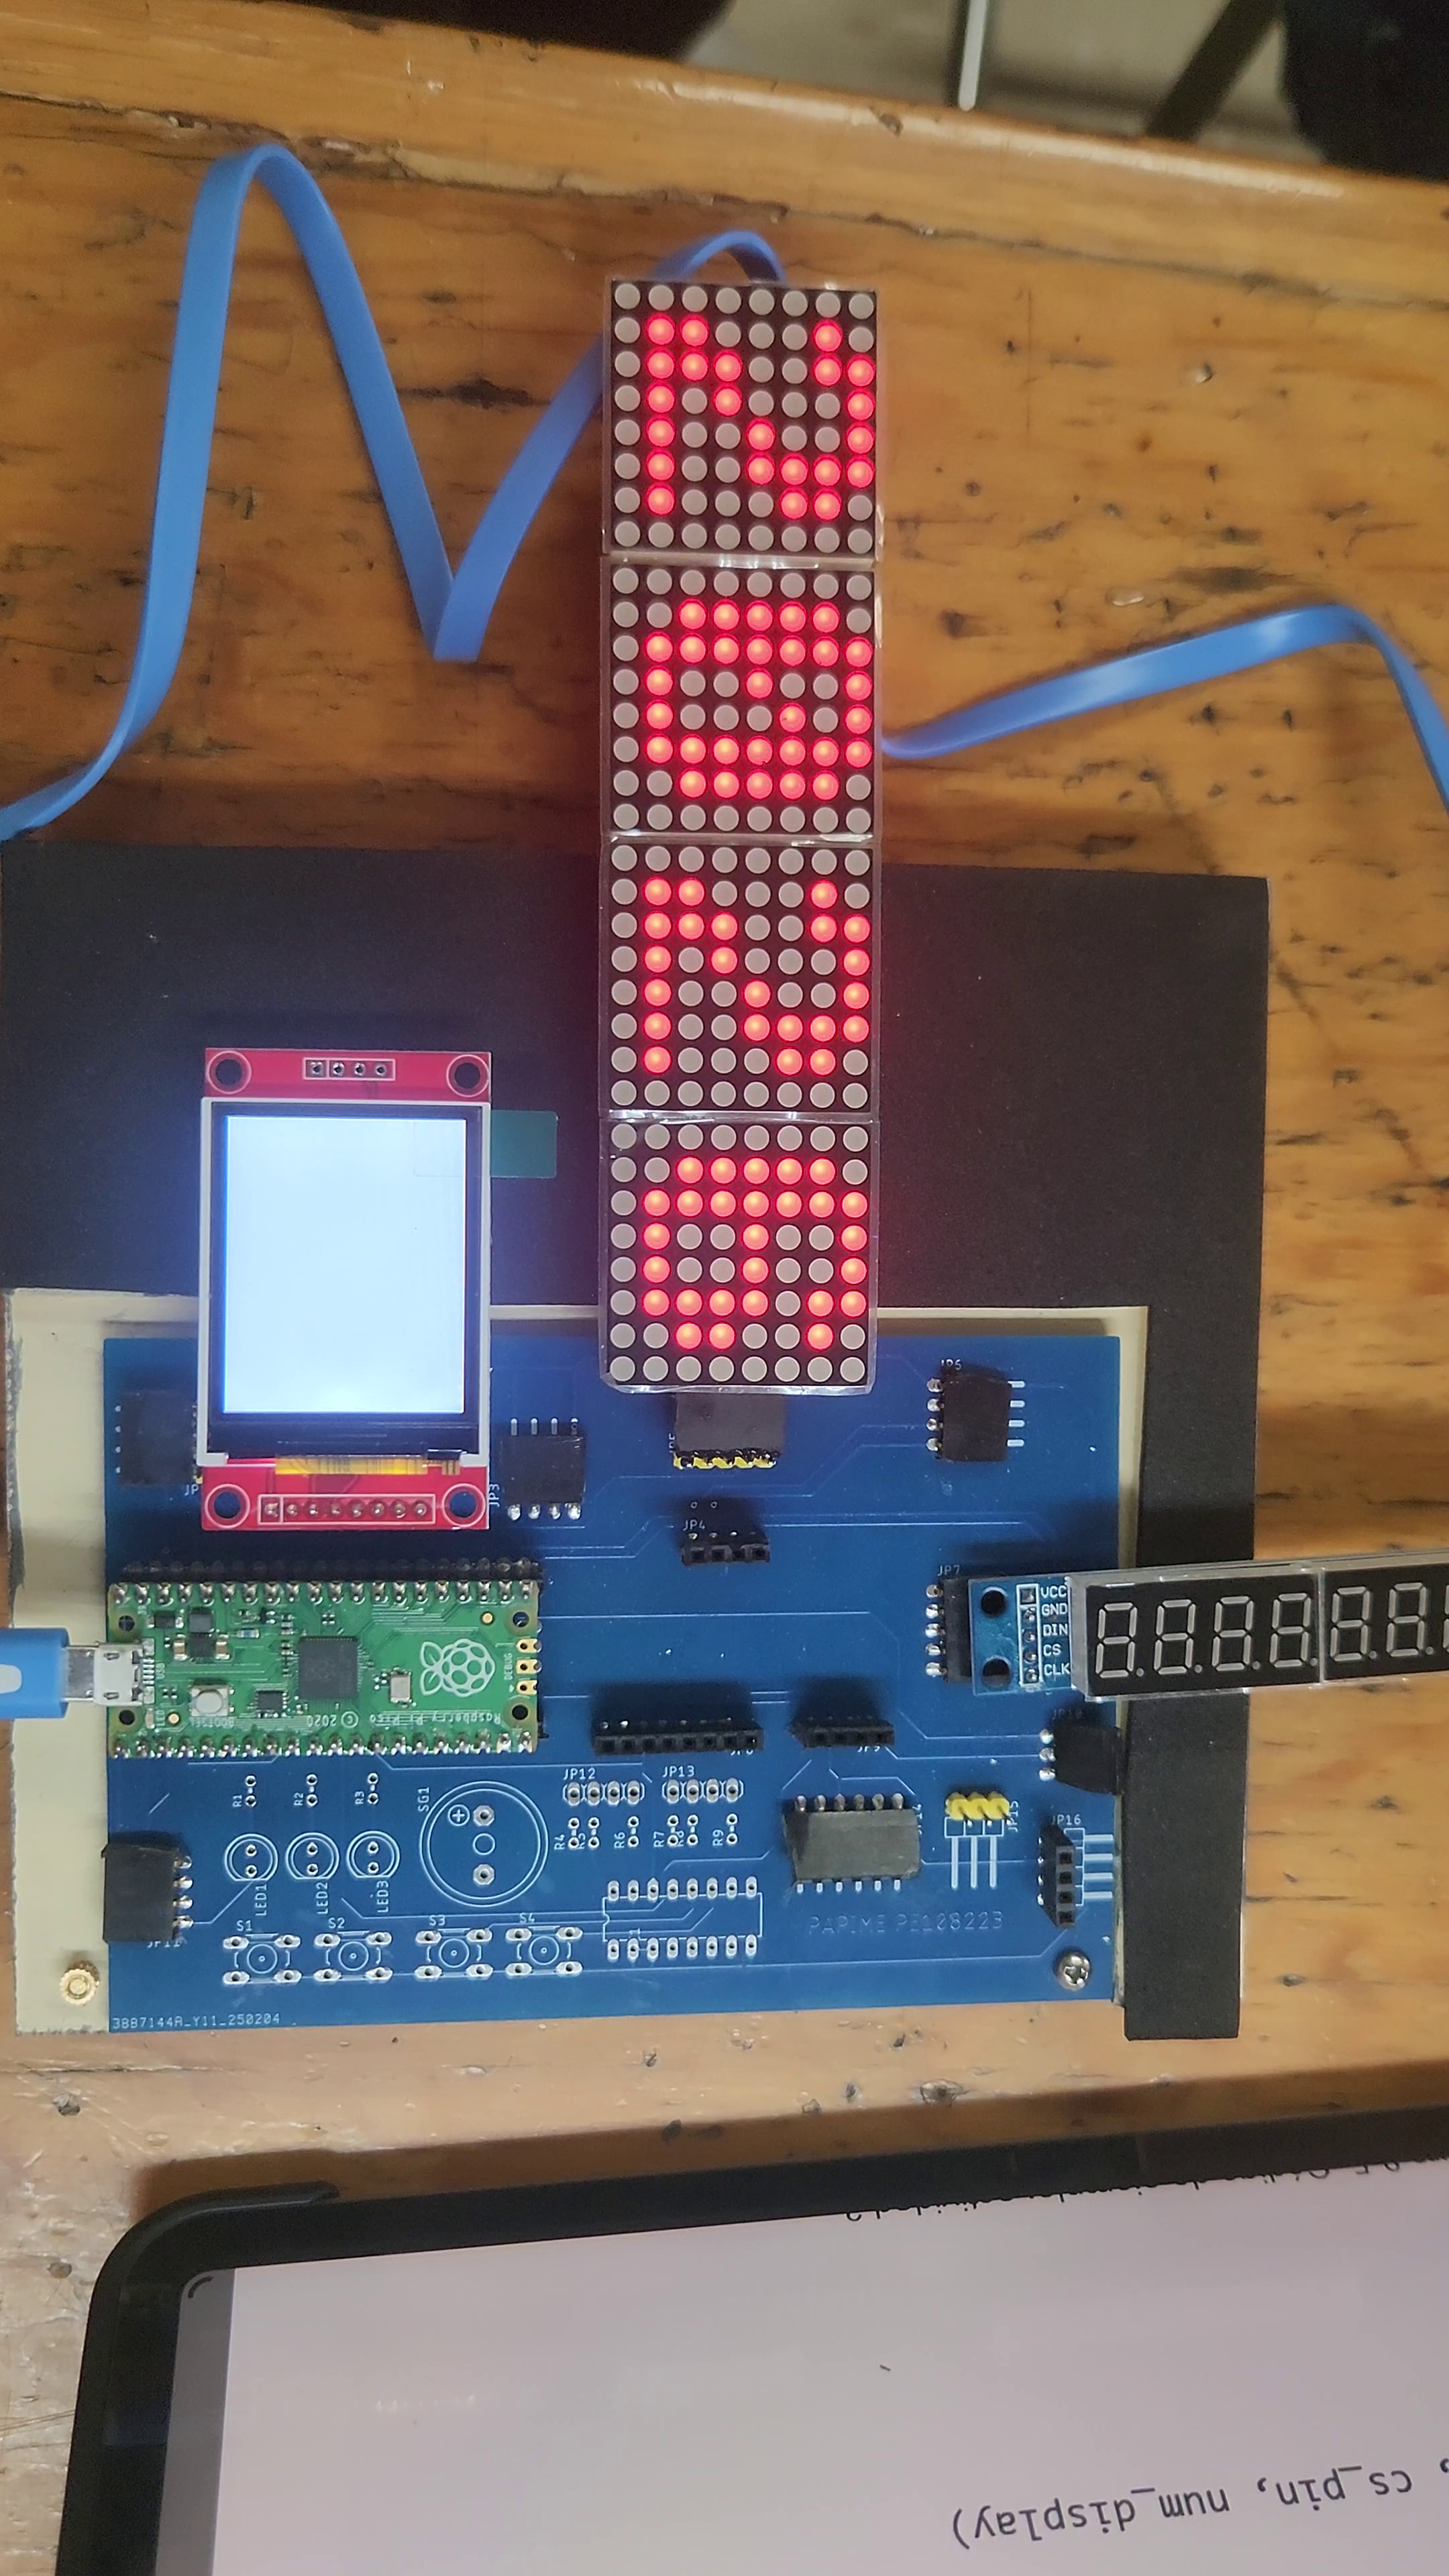
\includegraphics[width=0.5\textwidth, angle=90]{img/Actividad4/Act4_3.png}
        \caption{Despliegue de datos numéricos. El bucle alcanza la cadena "2026". El microcontrolador actualiza la pantalla evidenciando la correcta renderización de la fuente tipográfica asignada para números enteros.}
    \end{figure}

    \begin{figure}[H]
        \centering
        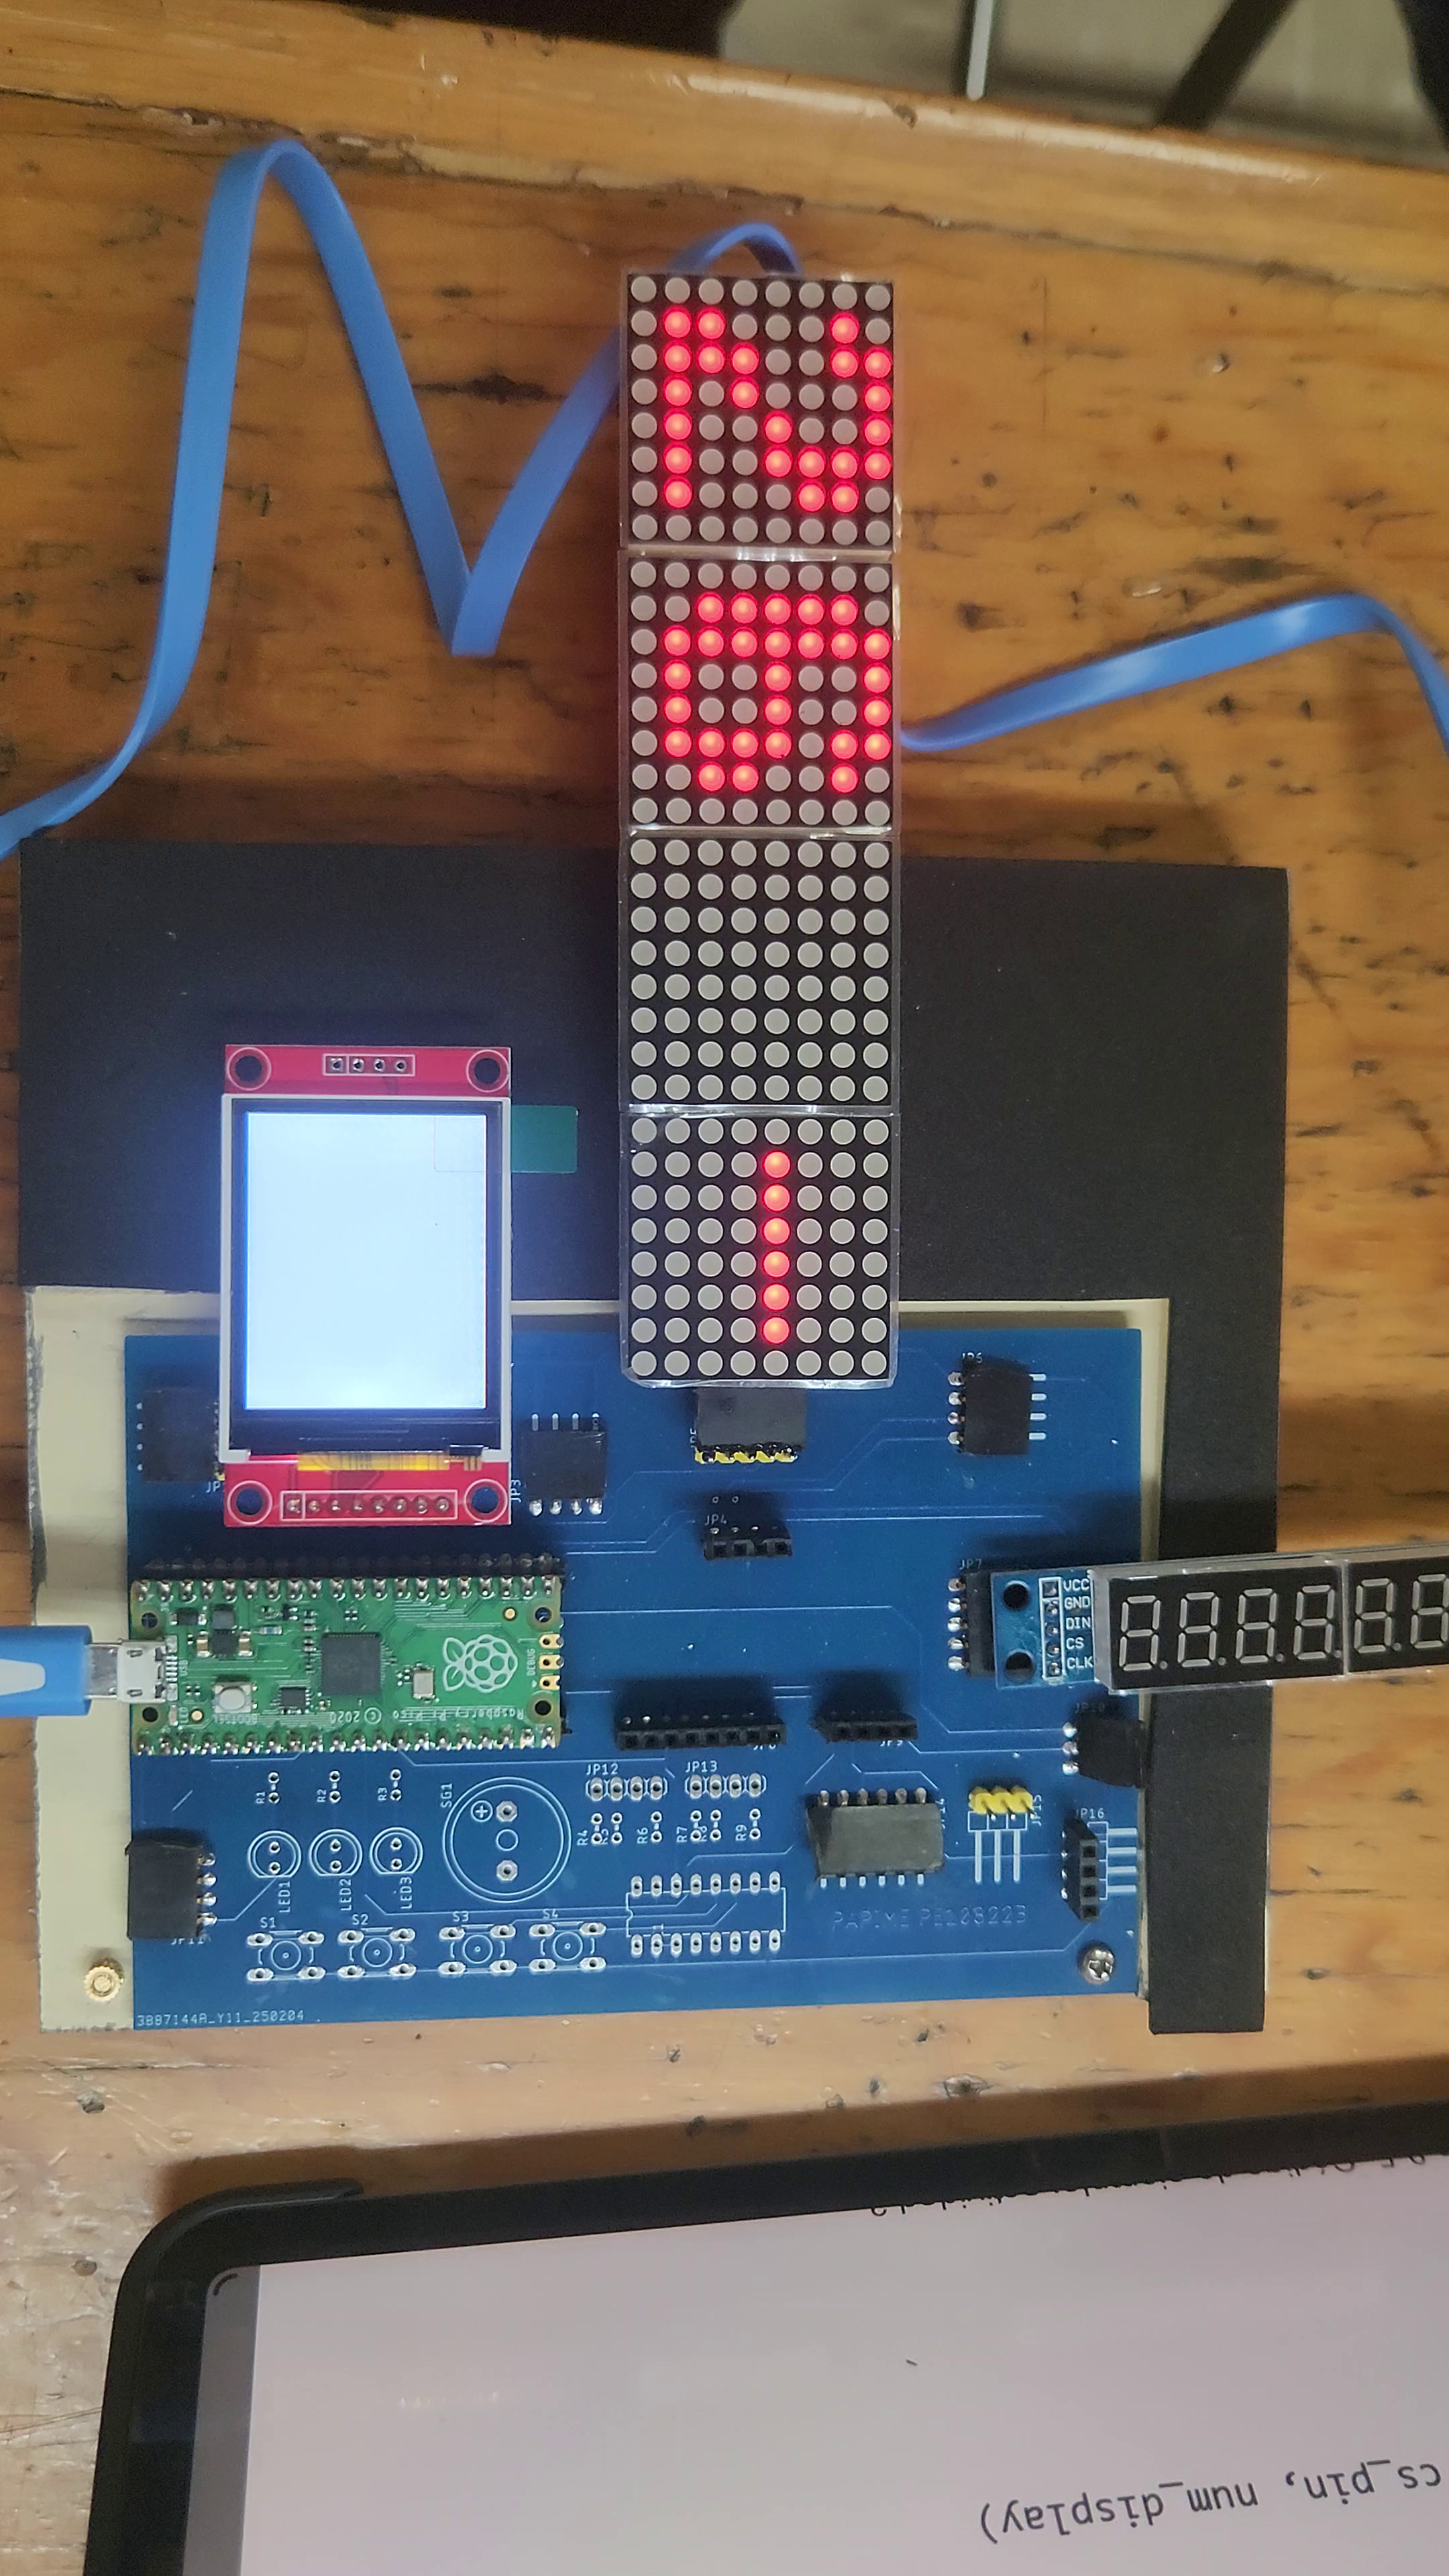
\includegraphics[width=0.4\textwidth, angle=90]{img/Actividad4/Act4_5.png}
        \caption{Despliegue de la cadena final. El bucle \texttt{for} carga el último elemento ("PEPE"). Los datos viajan por el bus y se enclavan en los registros del display, logrando iluminar el texto libre solicitado en el manual.}
    \end{figure}

    \begin{figure}[H]
        \centering
        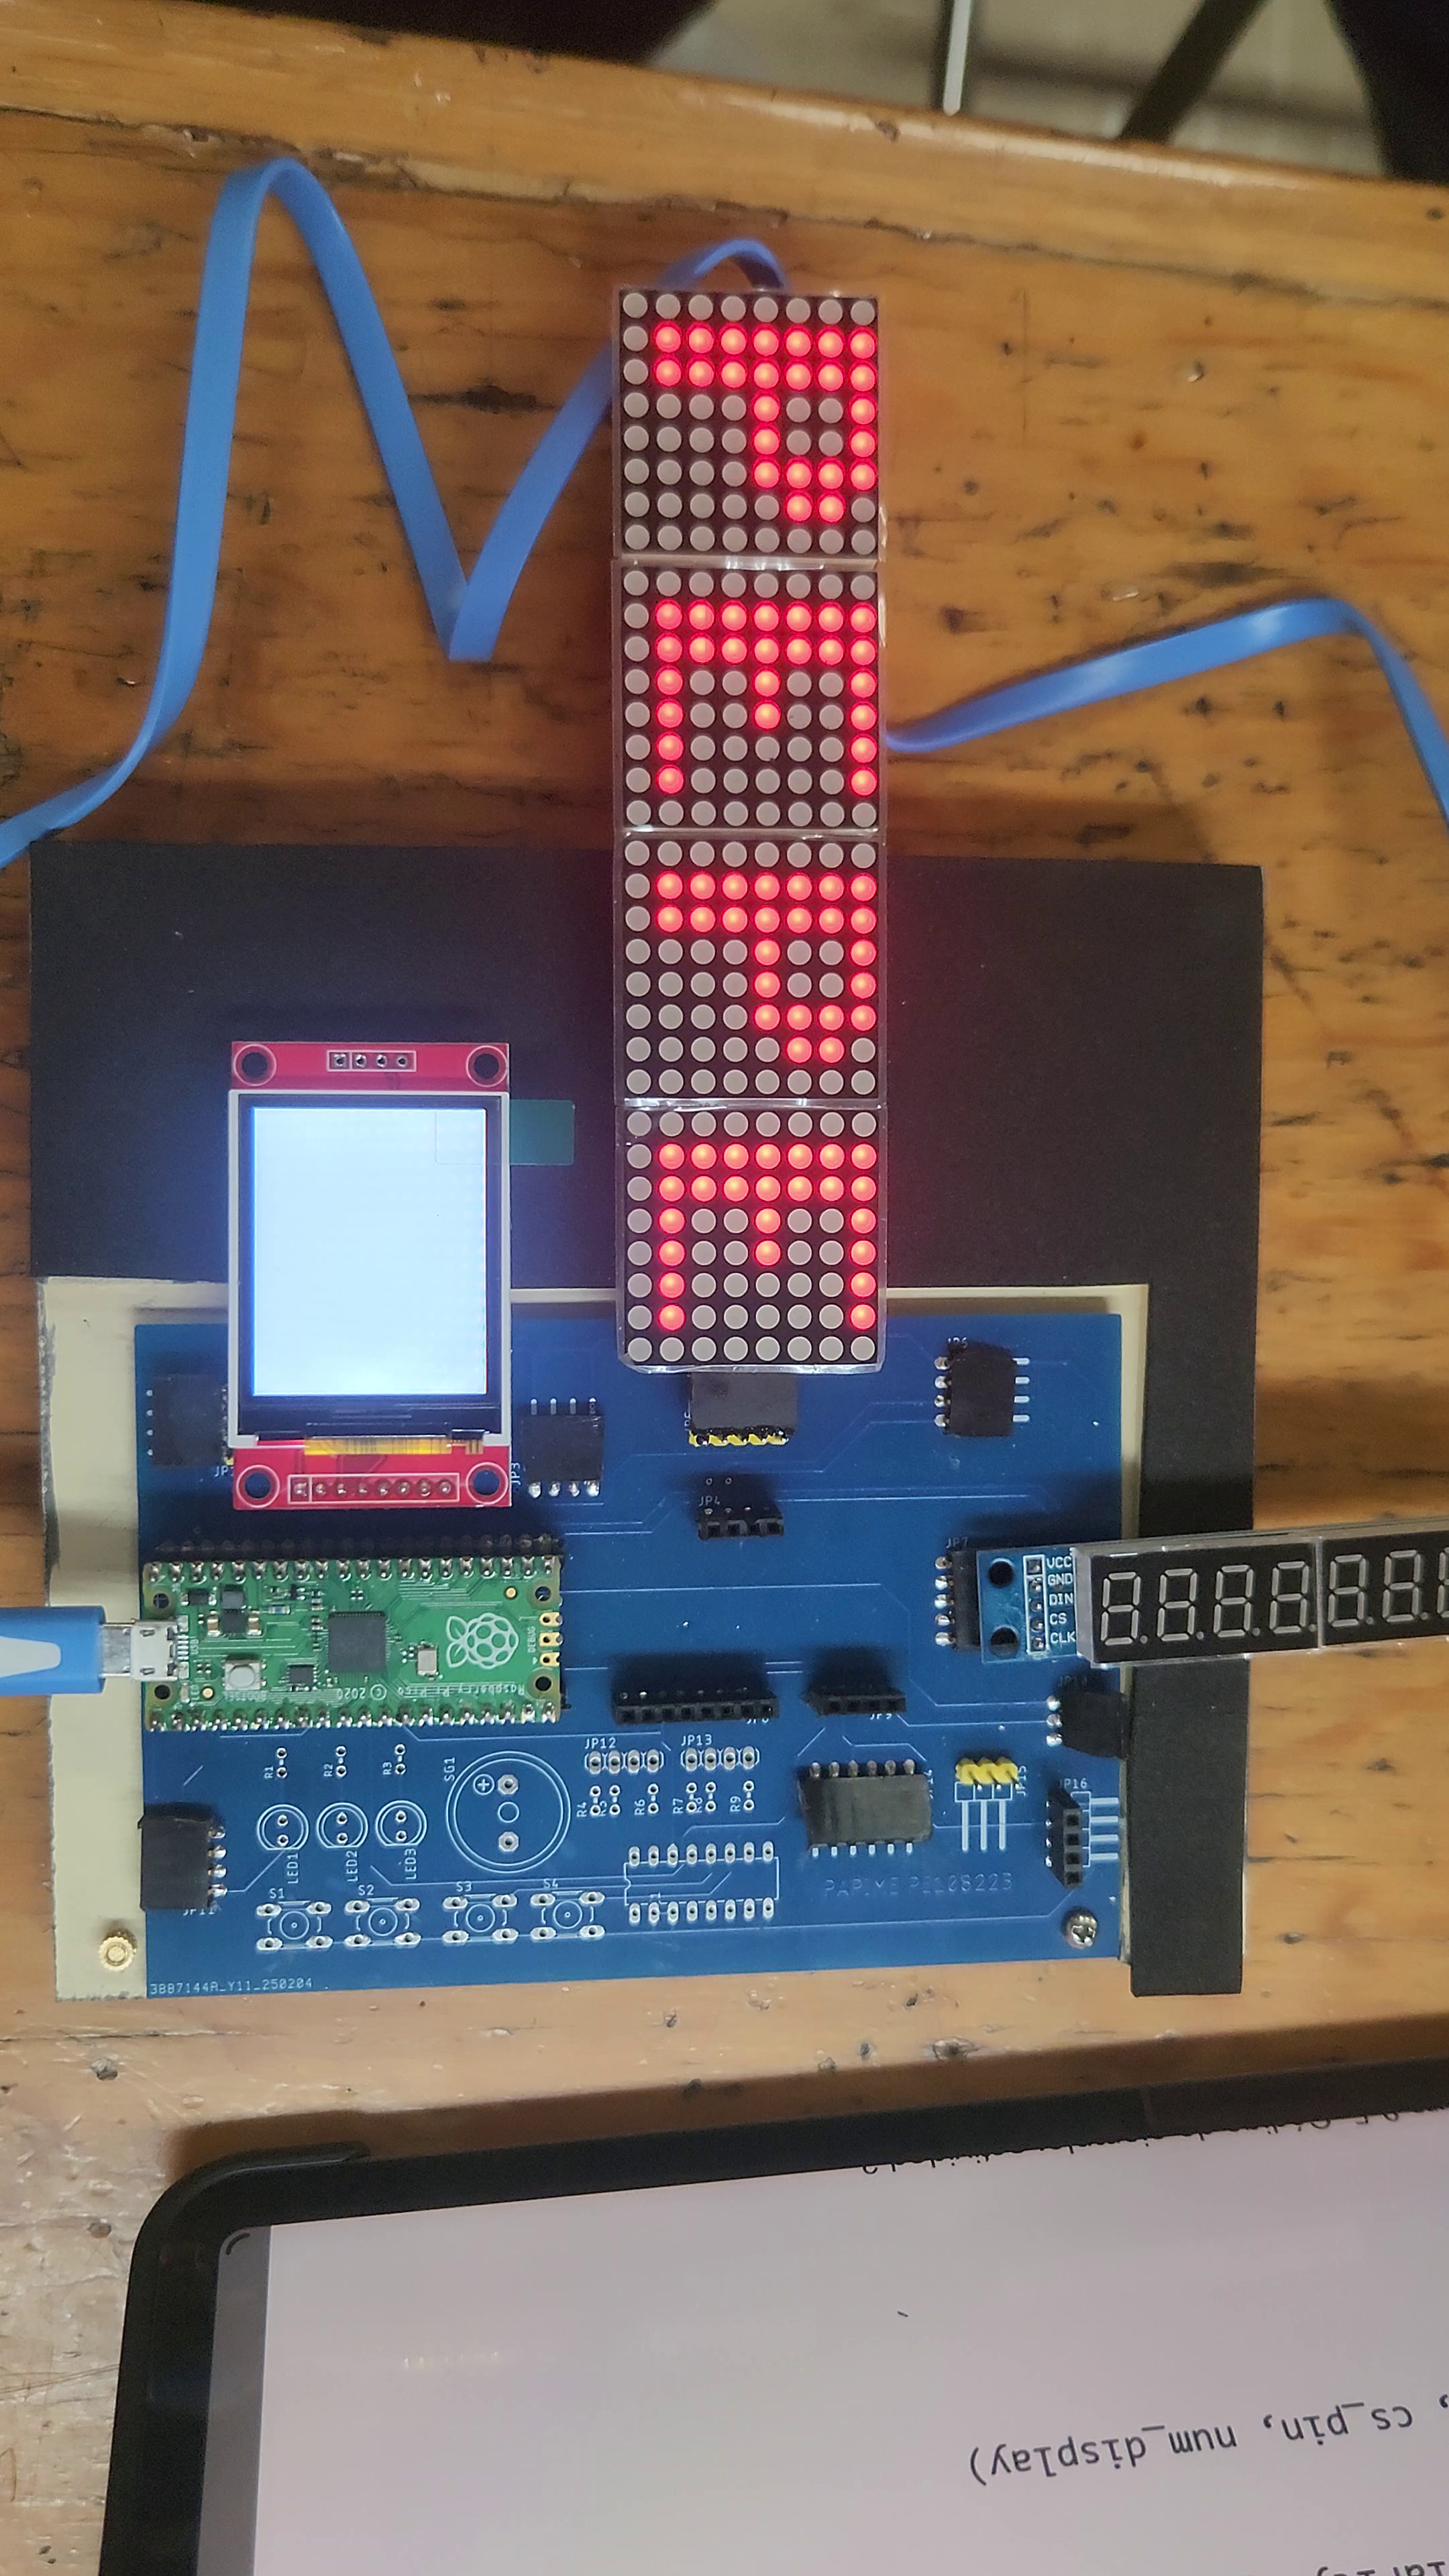
\includegraphics[width=0.4\textwidth, angle=90]{img/Actividad4/Act4_6.png}
        \caption{Reinicio del ciclo de visualización. El programa mantiene la cadena "PEPE" durante su temporización estipulada de 2 segundos antes de que el bucle infinito reinicie y vuelva a mandar la cadena inicial "UNAM", cerrando el lazo de ejecución.}
    \end{figure}

    \subsection*{Análisis de resultados}
    El código demuestra el manejo de un bus síncrono para controlar arreglos de LEDs. Al definir el parámetro \texttt{num\_display = 4} en la inicialización de la clase, la librería ajusta automáticamente la memoria de video (\textit{framebuffer}) para abarcar un ancho total de 32 columnas. 
    
    Durante la ejecución del ciclo, el microcontrolador envía las tramas de datos por la línea MOSI. La función \texttt{display.text()} se encarga de convertir cada letra de la cadena de texto en un mapa de bits que enciende los LEDs correspondientes. La instrucción \texttt{display.fill(0)} resulta fundamental, ya que apaga todos los puntos luminosos en la transición, garantizando un salto limpio entre un mensaje y otro. 
    El uso de la función de retardo pausa la actualización gráfica, cumpliendo de manera exacta con el ritmo de visualización establecido en la actividad.

    \newpage

    \section*{Actividad 5}

    Escribir el siguiente programa, cerciorarse que el módulo Display TFT ST7735, se
    encuentre conectado en la posición correcta; investigar el funcionamiento de las librerías usadas;
    comentar el programa.

    \begin{tikzpicture}

        % Llamada a la Raspberry Pi Pico
        \picoboard


        \node[text=blue!40!black, font=\large\sffamily\bfseries, align=center] at (-3.2, -0.5) {DISPLAY TFT\\[0.1cm]ST 7735};

        % Contorno del Módulo TFT
        \draw[thick] (-7.5, -1.3) rectangle (-4.0, -5.2);

        % Etiquetas internas (Alineadas a la derecha, en cursiva y negrita como en la imagen)
        \node[left, font=\normalsize\sffamily\bfseries] at (-4.0, -1.8) {SCK};
        \node[left, font=\normalsize\sffamily\bfseries] at (-4.0, -2.25) {MOSI};
        \node[left, font=\normalsize\sffamily\bfseries] at (-4.0, -2.9) {$\overline{CS}$};
        \node[left, font=\normalsize\sffamily\bfseries] at (-4.0, -3.9) {RESET};
        \node[left, font=\normalsize\sffamily\bfseries] at (-4.0, -4.7) {A0};

        % Etiqueta VCC, LED (Alineada a la izquierda superior)
        \node[right, font=\normalsize\sffamily\bfseries] at (-7.5, -1.8) {VCC, LED};

        % --- CONEXIONES A LA PICO ---
        
        % Conexión SCK (Azul Oscuro) a GP2 (Pin 4)
        \draw[blue!40!black, very thick] (-4.0, -1.8) -- (P4);
        
        % Conexión MOSI (Verde) a GP3 (Pin 5)
        \draw[green!50!black, very thick] (-4.0, -2.25) -- (P5);
        
        % Conexión CS (Roja) en diagonal a GP7 (Pin 10)
        \draw[red!80!black, very thick] (-4.0, -2.9) -- (P10);

        % --- CONEXIONES DE ENERGÍA ---

        % Conexión 3.3V (Cable rojo hacia arriba, barra verde horizontal)
        \draw[red, thick] (-7.0, -1.3) -- (-7.0, -0.6);
        \draw[green!60!black, thick] (-7.4, -0.6) -- (-6.6, -0.6);
        \node[above, font=\small\sffamily\bfseries] at (-7.0, -0.6) {3.3V};

        % Conexión GND inferior
        % Línea negra vertical
        \draw[very thick] (-4.6, -5.2) -- (-4.6, -6.1);
        % Pequeño detalle verde justo antes de la tierra (como en la imagen original)
        \draw[green!60!black, thick] (-4.6, -6.1) -- (-4.6, -6.3);
        
        % Símbolo de Tierra (GND)
        \draw[thick] (-5.0, -6.3) -- (-4.2, -6.3);
        \draw[thick] (-4.8, -6.45) -- (-4.4, -6.45);
        \draw[thick] (-4.65, -6.6) -- (-4.55, -6.6);
        
        % Etiqueta GND externa
        \node[right, font=\normalsize\sffamily\bfseries] at (-4.5, -5.6) {GND};

    \end{tikzpicture}


    \subsection*{Propuesta de solución}
    El objetivo es desplegar texto a color en un panel LCD TFT. A diferencia de las matrices simples, esta pantalla requiere una comunicación SPI de alta velocidad (20 MHz) y el uso de terminales adicionales de control. Se define el pin A0 (o DC) para que el controlador ST7735 pueda distinguir si los datos entrantes son comandos de configuración o píxeles de imagen, además de un pin físico para el RESET.
    
    La solución emplea la librería \texttt{ST7735} para manejar la secuencia de encendido del hardware. Posteriormente, se ajusta la orientación de la pantalla al modo apaisado (\textit{landscape}), se corrige la paleta de colores si es necesario, y se pinta un fondo blanco sólido para asegurar el contraste. Finalmente, se envían dos cadenas de texto estáticas ("MICROS" y "FI") asignándoles coordenadas, colores específicos y una escala de tamaño definida para que resalten en el panel.

    \begin{center}
    \begin{tikzpicture}[
        node distance=5mm and 12mm, % <-- Distancia vertical reducida
        every node/.style={font=\footnotesize\sffamily} % <-- Fuente un poco más pequeña
    ]
        \node (inicio) [startstop] {Inicio};
        \node (spi) [process, below=of inicio, text width=5.5cm, align=center] {Configurar \texttt{SPI(0)}\\ a 20 MHz con pines SCK, MOSI y MISO};
        \node (objeto) [process, below=of spi, text width=5.5cm, align=center] {Crear el objeto \texttt{TFT}\\ con A0=15, RESET=14 y CS=5};
        \node (init) [process, below=of objeto, text width=5.5cm, align=center] {Inicializar el controlador\\ con \texttt{tft.initg()}};
        \node (rgb) [process, below=of init, text width=5.5cm, align=center] {Corregir el orden de color\\ con \texttt{tft.rgb(True)}};
        \node (rot) [process, below=of rgb, text width=5.5cm, align=center] {Fijar orientación\\ con \texttt{tft.rotation(2)}};
        \node (fondo) [process, below=of rot, text width=5.5cm, align=center] {Pintar fondo blanco\\ con \texttt{tft.fill(TFT.WHITE)}};
        \node (txt1) [process, below=of fondo, text width=5.5cm, align=center] {Escribir \texttt{"MICROS"}\\ en rojo, escala 2, posición (10,10)};
        \node (txt2) [process, below=of txt1, text width=5.5cm, align=center] {Escribir \texttt{"FI"}\\ en verde, escala 2, posición (25,30)};
        \node (fin) [startstop, below=of txt2] {Fin};

        \draw [arrow] (inicio) -- (spi);
        \draw [arrow] (spi) -- (objeto);
        \draw [arrow] (objeto) -- (init);
        \draw [arrow] (init) -- (rgb);
        \draw [arrow] (rgb) -- (rot);
        \draw [arrow] (rot) -- (fondo);
        \draw [arrow] (fondo) -- (txt1);
        \draw [arrow] (txt1) -- (txt2);
        \draw [arrow] (txt2) -- (fin);
    \end{tikzpicture}
    \end{center}

    \noindent El flujo de datos es estrictamente secuencial: el RP2040 crea primero la interfaz SPI y después envía comandos de configuración al ST7735 para inicializarlo, corregir el orden de color y fijar la rotación. Una vez establecida la pantalla, se transmite un bloque de color sólido para el fondo y, al final, dos tramas de texto con coordenadas, escala y color distintos. Como no hay bucles ni condiciones en este script, la secuencia se ejecuta una sola vez y la imagen queda estática en el display.

    \subsection*{Desarrollo}

    \lstinputlisting[language={[LAB]Python}, caption=Código de la Actividad 5, basicstyle=\ttfamily\scriptsize]{Code/Act5.py}


    \begin{figure}[H]
        \centering
        
\includegraphics[width=0.5\textwidth]{img/Actividad5/Act5_1.jpg}
        \caption{Despliegue gráfico en el panel TFT ST7735. El microcontrolador inicializa la comunicación SPI a 20 MHz y reconfigura la orientación geométrica de la pantalla a modo apaisado (\texttt{rotation(2)}). Se comprueba el control directo, el fondo de color blanco (\texttt{fill}) y renderizar las cadenas estáticas "MICROS" (en color rojo) y "FI" (en color verde).}
    \end{figure}

    \subsection*{Análisis de resultados}
    Al cargar el script, el microcontrolador inicializa la pantalla TFT de forma exitosa mediante \texttt{tft.initg()}. Esta instrucción manda la secuencia de voltajes y comandos necesarios para despertar el panel. La línea \texttt{tft.rgb(True)} resulta clave para el correcto despliegue visual, ya que en algunos de estos módulos los canales de color rojo y azul vienen invertidos de fábrica (formato BGR en lugar de RGB); este parámetro corrige esa desviación por software.

    La instrucción \texttt{tft.rotation(2)} reordena las direcciones de la memoria gráfica, lo que voltea la imagen para que coincida con la disposición horizontal en la que suele montarse la pantalla físicamente. A continuación, \texttt{tft.fill(TFT.WHITE)} inunda todos los píxeles de blanco. Por último, la función \texttt{tft.text()} traduce las letras a puntos de color rojo y verde en las posiciones (10, 10) y (25, 30), 
    escalando la fuente a tamaño 2. Esto comprueba que el RP2040 puede gestionar gráficos y colores de manera directa utilizando librerías dedicadas.

    \newpage

    \section*{Actividad 6}

    Realizar un programa que muestre los nombres de cada integrante de su equipo; elegir el formato que desee, así como el color para cada campo.

    \begin{center}
    \begin{tikzpicture}
        % Rectángulo exterior
        \draw[ultra thick] (0,0) rectangle (4.5, 6);
        
        % Textos en posiciones específicas
        \node[font=\sffamily\large\bfseries, text=black, anchor=west] at (0.2, 5.2) {Texto 1};
        \node[font=\sffamily\large\bfseries, text=blue!70!black, anchor=west] at (1.4, 4.1) {Texto 2};
        \node[font=\sffamily\large\bfseries, text=red, anchor=west] at (0.2, 3.0) {Texto 3};
        \node[font=\sffamily\large\bfseries, text=green!70!black, anchor=west] at (1.6, 1.9) {Texto 4};
        
        % Texto 5 rotado -90 grados (escrito de arriba hacia abajo)
        \node[font=\sffamily\large\bfseries, text=orange!90!yellow, rotate=-90, anchor=west] at (3.8, 3.2) {Texto 5};
    \end{tikzpicture}

    \vspace{10pt}
    \sffamily Figura 8-8. Despliegue propuesto; actividad 6
    \end{center}


    \subsection*{Propuesta de solución}

    Dado que se va a trabajar con una pantalla TFT, es necesario importar la biblioteca \texttt{ST7735} para controlar el display. De igual modo se hace uso de la biblioteca \texttt{machine} especificamente para los módulos \texttt{SPI} y \texttt{Pin} para configurar la comunicación SPI y los pines de control. Se define el bus SPI con una frecuencia de 20 MHz, asignando los pines correspondientes para SCK, MOSI y MISO.

    El paso siguiente es realizar la configuración del display donde se debe crear un objeto de la clase \texttt{TFT} con los parámetros de pin de Datos/Comando, reset, y el CS. Luego se inicializa el display con \texttt{tft.initg()}, se corrige el orden de color con \texttt{tft.rgb(True)}, se fija la orientación con \texttt{tft.rotation(1)} para usar la pantalla en modo horizontal, ya con la pantalla configurada se pinta un fondo negro con \texttt{tft.fill(TFT.BLACK)} para asegurar un buen contraste.

    Ya con la pantalla y el fondo de color de la misma se procede a realizar la escritura del nombre de los integrantes del equipo, debido a la longitud del tamaño de los nombres, se opto por usar abreviaturas o pseudónimos. Para colocar texto en pantalla se hace uso del método \texttt{tft.text(Coord, Nombre, Color, TipoLetra, Tamaño, AjusteLinea)}. De forma que usando este comando se colocaron los nombres del equipo, donde para que el texto no se amontonara o se viera de un mismo color los argumentos que se cambiaron por cada nombre es \texttt{Coord} donde la coordenada en Y se incremento de 20 en 20, el nombre con el texto correspondiente, el color, y el tamaño de fuente solo se modifico cuando se coloco el texto correspondiente al número de equipo para que destacara.

    \begin{figure}[H]
        \begin{tikzpicture}[
            scale=1.0, transform shape,
            node distance=8mm and 12mm,
            every node/.style={font=\small\sffamily},
            % Definición de estilos de nodos
            startstop/.style={rectangle, rounded corners, draw=black, fill=red!20, minimum width=3cm, minimum height=1cm, text centered},
            process/.style={rectangle, draw=black, fill=orange!20, minimum width=3cm, minimum height=1cm, text centered, align=center},
            arrow/.style={thick, ->, >=stealth}
        ]

            % --- Declaración de Nodos ---
            \node (inicio) [startstop] {Inicio};
            
            \node (spi) [process, below=of inicio, text width=5.5cm] {Configurar bus \texttt{SPI(0)}\\ Pines SCK=2, MOSI=3, MISO=4};
            
            \node (tft) [process, below=of spi, text width=6cm] {Inicializar display \texttt{TFT} (CS = Pin 7)\\ Activar RGB y modo apaisado};
            
            \node (fondo) [process, below=of tft, text width=4.5cm] {Limpiar la pantalla:\\ \texttt{tft.fill(TFT.BLACK)}};
            
            \node (nombres) [process, below=of fondo, text width=6cm] {Escribir lista de nombres:\\ \texttt{"Perci", "Tenshi", "Victor", "Fofo"}\\ (Con diferentes colores y eje Y)};
            
            \node (titulo) [process, below=of nombres, text width=5.5cm] {Escribir título:\\ \texttt{"Equipo 6"} en (5, 100)\\ Tamaño de fuente: Escala 2};
            
            \node (fin) [startstop, below=of titulo] {Fin};

            % --- Conexiones Lineales ---
            \draw [arrow] (inicio) -- (spi);
            \draw [arrow] (spi) -- (tft);
            \draw [arrow] (tft) -- (fondo);
            \draw [arrow] (fondo) -- (nombres);
            \draw [arrow] (nombres) -- (titulo);
            \draw [arrow] (titulo) -- (fin);

        \end{tikzpicture}
        \centering
    \end{figure}


    \subsection*{Desarrollo}

    \lstinputlisting[language={[LAB]Python}, caption=Código de la Actividad 6,basicstyle=\ttfamily\scriptsize]{Code/Act6.py}


    \begin{figure}[H]
        \centering
        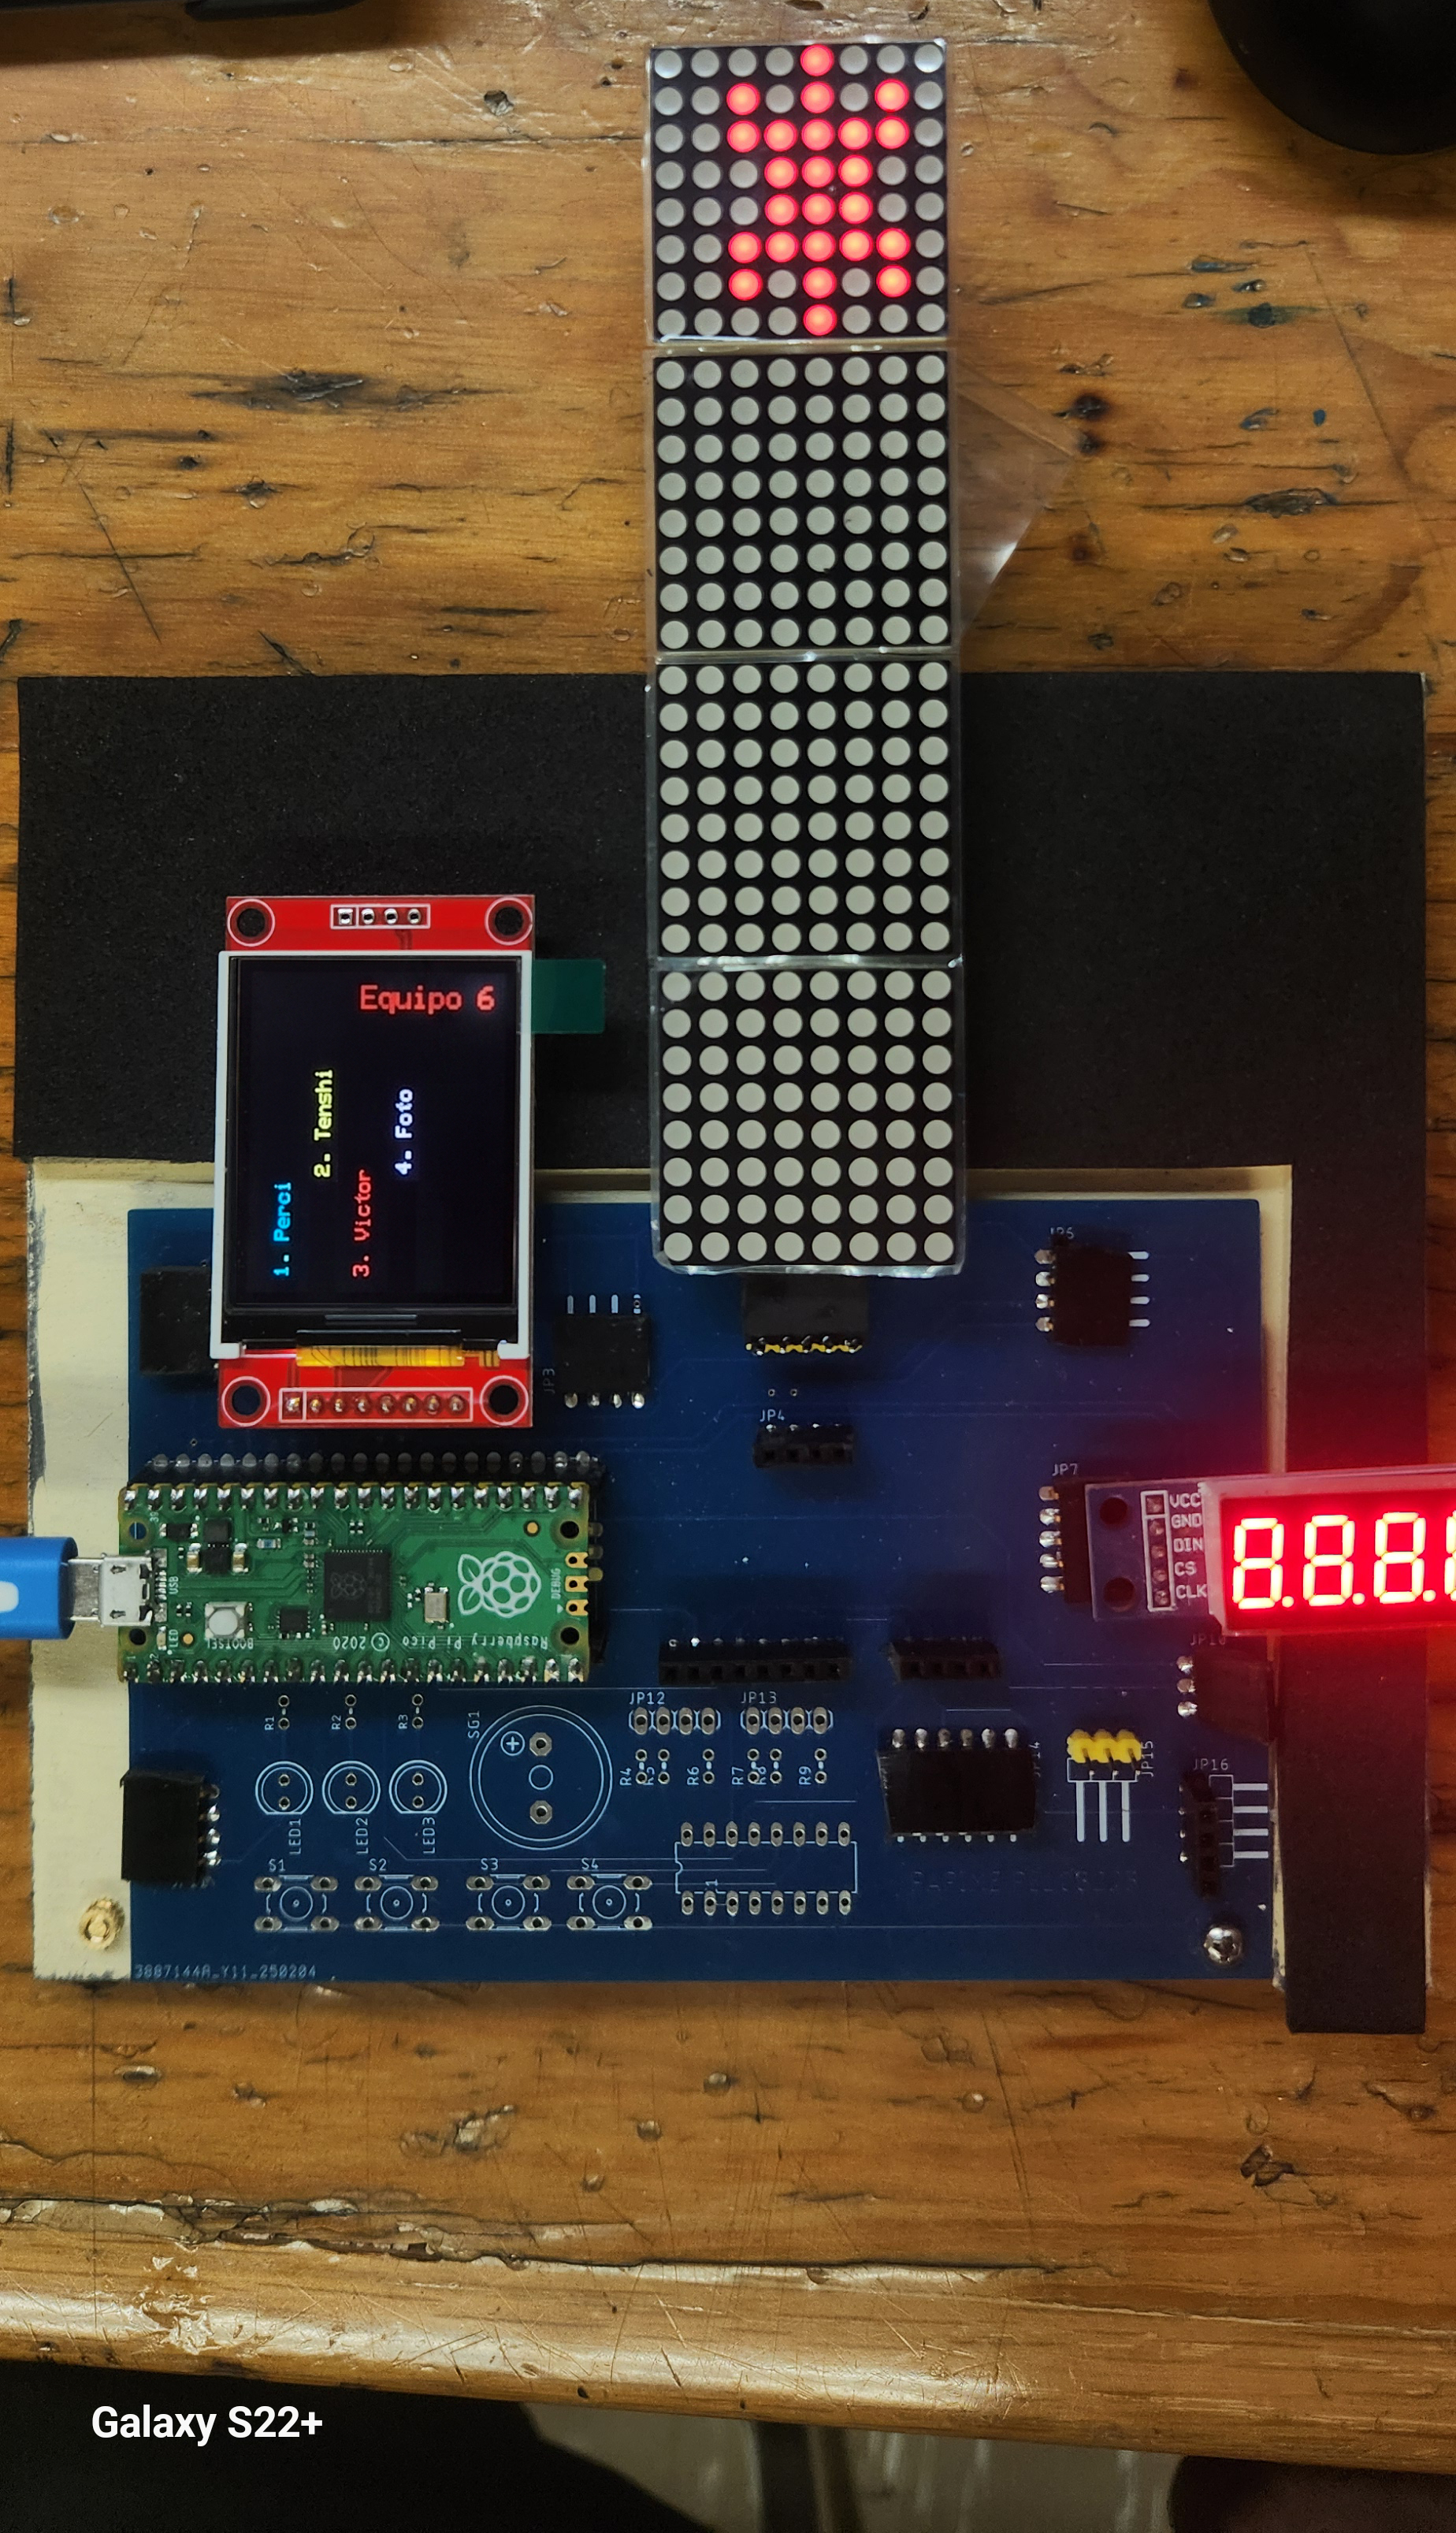
\includegraphics[width=0.5\textwidth, angle=-90]{img/Actividad6/Act6_1.png}
        \caption{Actividad 6:Despliegue gráfico en el panel TFT ST7735, mostrando los nombres de cada integrante del equipo}
    \end{figure}

    \subsection*{Análisis de resultados}

    A partir de la imagen obtendida se puede observar que el programa logra desplegar los nombres de cada integrante del equipo, usando diferentes colores para cada nombre y un título con un tamaño de fuente más grande para destacar el número de equipo. A demás los textos se encuentran bien distribuidos en la pantalla, evitando que se amontonen y asegurando una buena legibilidad. Por lo que para mostrar texto en el display TFT se hizo uso del método \texttt{tft.text()} que permite colocar texto en coordenadas específicas, con un color y tamaño de fuente determinado, lo que facilita la personalización del despliegue gráfico así como personalizar el formato de presentación de la información. Ya que se podrían importar fuentes tipográficas adicionales para usar en el display, o incluso crear gráficos personalizados para acompañar el texto, aprovechando la capacidad de color y resolución del panel TFT.

    \newpage
    \section*{Actividad 7}

    Realizar un programa que muestre el valor del contador generado por dos entradas
    digitales, tal como se muestra en la tabla 8-3; el contador debe mostrarse en los tres dispositivos
    utilizados en esta práctica (Display TFT, Matriz 4x8x8 y el Display de 8 dígitos) al mismo tiempo.

    \begin{tikzpicture}[
        scale=0.65, transform shape,
        pin_label/.style={font=\sffamily\bfseries\small},
        title_label/.style={font=\sffamily\bfseries\large, text=blue!60!black},
        dest_label/.style={font=\sffamily\bfseries\normalsize, text=black},
        break_label/.style={font=\sffamily\bfseries\small, fill=white, inner sep=1.5pt} 
    ]


        \picoboard

        \node[title_label, anchor=south west] at (-11.5, -0.2) {Display 8 dígitos};
        
        % Caja principal
        \draw[thick] (-11.5, -0.5) rectangle (-4.5, -3.5);
        
        % Rectángulos de los 8 dígitos
        \foreach \i in {0,...,7} {
            \draw[thick] (-11.2 + \i*0.8, -0.8) rectangle ++(0.65, -2.4);
        }

        % Conexión VCC 
        \draw[red, thick] (-6.5, -0.5) -- (-6.5, 0.5) -- (-5.5, 0.5);
        \node[break_label] at (-6.5, -0.5) {VCC};
        \node[above, pin_label] at (-6.5, 0.5) {5V};
        \node[right, pin_label] at (-5.5, 0.5) {VBUS};

        % Conexión GND
        \draw[thick] (-6.5, -3.5) -- (-6.5, -4.5);
        \node[break_label] at (-6.5, -3.5) {GND};
        
        % Símbolo de Tierra
        \draw[thick] (-7.0, -4.5) -- (-6.0, -4.5);
        \draw[thick] (-6.8, -4.65) -- (-6.2, -4.65);
        \draw[thick] (-6.6, -4.8) -- (-6.4, -4.8);
        \node[right, pin_label] at (-6.0, -4.65) {GND};

        % Conexiones laterales derechas
        \draw[blue!40!black, very thick] (-4.5, -1.8) -- (0, -1.8);
        \node[above, pin_label] at (-3.7, -1.8) {SCK};
        
        \draw[green!60!black, very thick] (-4.5, -2.5) -- (0, -2.5);
        \node[below, pin_label] at (-3.7, -2.5) {MOSI};
        
        \draw[red!80!black, very thick] (-4.5, -3.2) -- (0, -3.2);
        \node[below, pin_label] at (-3.7, -3.2) {$\overline{SS}$};



        \node[title_label, anchor=south west] at (-11.5, -6.2) {Matriz 8x8 x 4};
        
        % Caja principal
        \draw[thick] (-11.5, -6.5) rectangle (-4.5, -9.5);
        
        % Las 4 matrices cuadradas
        \foreach \i in {0,...,3} {
            \draw[thick] (-11.1 + \i*1.6, -6.8) rectangle ++(1.3, -2.4);
        }

        % Conexión VCC
        \draw[red, thick] (-6.5, -6.5) -- (-6.5, -5.5) -- (-5.5, -5.5);
        \node[break_label] at (-6.5, -6.5) {VCC};
        \node[above, pin_label] at (-6.5, -5.5) {5V};
        \node[right, pin_label] at (-5.5, -5.5) {VBUS};

        % Conexión GND
        \draw[thick] (-6.5, -9.5) -- (-6.5, -10.5);
        \node[break_label] at (-6.5, -9.5) {GND};
        
        % Símbolo de Tierra
        \draw[thick] (-7.0, -10.5) -- (-6.0, -10.5);
        \draw[thick] (-6.8, -10.65) -- (-6.2, -10.65);
        \draw[thick] (-6.6, -10.8) -- (-6.4, -10.8);
        \node[right, pin_label] at (-6.0, -10.65) {GND};

        % Conexiones laterales derechas 
        \draw[blue!40!black, very thick] (-4.5, -7.5) -- (-2.5, -7.5) node[right, dest_label] {GP2};
        \node[above, pin_label] at (-3.7, -7.5) {CLK};
        
        \draw[green!60!black, very thick] (-4.5, -8.2) -- (-2.5, -8.2) node[right, dest_label] {GP3};
        \node[below, pin_label] at (-3.7, -8.2) {MOSI};
        
        \draw[red!80!black, very thick] (-4.5, -8.9) -- (-2.5, -9.4) node[right, dest_label] {GP6};
        \node[below, pin_label] at (-3.7, -9.2) {$\overline{CS}$};



        \node[title_label, align=center] at (9.0, 0.2) {DISPLAY TFT\\[0.1cm]ST 7735};
        
        % Caja principal
        \draw[thick] (6.5, -0.8) rectangle (10.5, -5.5);

        % Textos internos derechos
        \node[left, pin_label, font=\sffamily\bfseries\itshape\normalsize] at (10.5, -1.8) {SCK};
        \node[left, pin_label, font=\sffamily\bfseries\itshape\normalsize] at (10.5, -2.25) {MOSI};
        \node[left, pin_label, font=\sffamily\bfseries\itshape\normalsize] at (10.5, -3.0) {$\overline{CS}$};
        \node[left, pin_label, font=\sffamily\bfseries\itshape\normalsize] at (10.5, -4.0) {RESET};
        \node[left, pin_label, font=\sffamily\bfseries\itshape\normalsize] at (10.5, -4.8) {A0};

        % Conexiones laterales
        \draw[blue!40!black, very thick] (10.5, -1.8) -- (12.0, -1.8) node[right, dest_label] {GP2};
        \draw[green!60!black, very thick] (10.5, -2.25) -- (12.0, -2.25) node[right, dest_label] {GP3};
        \draw[red!80!black, very thick] (10.5, -3.0) -- (12.5, -3.8) node[right, dest_label] {GP7};

        % Textos VCC
        \node[right, pin_label, font=\sffamily\bfseries\itshape\normalsize] at (6.5, -1.2) {VCC};
        \node[left, pin_label, font=\sffamily\bfseries\itshape\normalsize] at (10.5, -1.2) {VCC, LED};

        % Conexión 3.3V
        \draw[red, thick] (7.2, -0.8) -- (7.2, 0.0);
        \draw[green!60!black, thick] (6.8, 0.0) -- (7.6, 0.0);
        \node[above, pin_label] at (7.2, 0.0) {3.3V};

        % Conexión GND inferior
        \draw[thick] (9.5, -5.5) -- (9.5, -6.1);
        \draw[green!60!black, thick] (9.5, -6.1) -- (9.5, -6.3);
        \draw[thick] (9.0, -6.3) -- (10.0, -6.3);
        \draw[thick] (9.2, -6.45) -- (9.8, -6.45);
        \draw[thick] (9.4, -6.6) -- (9.6, -6.6);
        \node[right, pin_label, font=\sffamily\bfseries\itshape\normalsize] at (9.8, -5.8) {GND};

    \end{tikzpicture}

    \begin{center}
    \begin{tikzpicture}
        % Se encierra la tabla en un nodo para dibujar la llave al lado
        \node (tbl1) [inner sep=0pt] {
            \setlength{\tabcolsep}{8pt}
            \renewcommand{\arraystretch}{1.3}
            \arrayrulecolor{white} % Líneas separadoras en blanco
            
            \begin{tabular}{>{\columncolor{hdrblue}\color{white}\bfseries}l | l | l}
            \rowcolor{hdrblue}
            Control & \textcolor{white}{\textbf{Estado}} & \textcolor{white}{\textbf{Acción}} \\ \hline
            GPIO12 (Pull\_Up) & \cellcolor{row1blue}Cerrado & \cellcolor{row1blue}Inicia/Reinicia cuenta \\ \hline
            GPIO13 (Pull\_Up) & \cellcolor{row2blue}Cerrado & \cellcolor{row2blue}Detiene cuenta \\ 
            \end{tabular}
        };
        
        % Llave decorativa a la derecha
        \draw [hdrblue, very thick, decorate, decoration={brace, amplitude=6pt, raise=4pt}]
        (tbl1.north east) -- (tbl1.south east)
        node [midway, right=14pt, align=left, font=\itshape, text=black] {Display TFT\\Matriz\\Display de 8 dígitos};
    \end{tikzpicture}

    \vspace{10pt}
    Tabla 8-3. Acciones de control; actividad 7
    \end{center}
    
    \newpage

    \section*{Propuesta de solución}
    Para controlar tres periféricos gráficos diferentes de forma simultánea, se implementa una topología de bus SPI compartido. El microcontrolador actúa como maestro y conecta sus únicas líneas de reloj (SCK) y datos (MOSI) a las tres pantallas en paralelo. La regla crítica de esta solución es asignar un pin de Selección de Chip (CS) exclusivo para cada módulo: GP5 para el display de 7 segmentos, GP6 para la matriz 8x8 y GP7 para la pantalla TFT. 
    
    El flujo del programa depende de botones físicos configurados con resistencias \textit{pull-up} internas. Al presionar el botón de inicio, se activa una bandera lógica que permite a un ciclo continuo aumentar un contador numérico. En cada iteración, el microcontrolador formatea el número como texto y lo envía secuencialmente a cada pantalla activando solo su pin CS correspondiente por breves fracciones de segundo. En la pantalla TFT, se dibuja el texto antiguo en color negro como método de "borrado rápido" antes de pintar el nuevo número, optimizando la velocidad del sistema.

    \noindent En el script actual, las decisiones de inicio y paro están modeladas como banderas lógicas fijas, por lo que la ruta activa entra a \texttt{corriendo} desde el primer ciclo. A partir de ahí, el contador se convierte en texto y se distribuye por SPI a los tres dispositivos usando su CS independiente; la TFT recibe un refresco doble, primero en \texttt{CYAN} y luego en \texttt{BLACK}, para borrar la cifra anterior sin limpiar toda la pantalla.

    \begin{center}
    \begin{tikzpicture}[
        scale=0.75, transform shape, % Reduce el tamaño de todo el diagrama al 75%
        node distance=5mm and 10mm,
        every node/.style={font=\footnotesize\sffamily}
    ]
        % --- Tronco Central Superior ---
        \node (inicio) [startstop] {Inicio};
        \node (spi) [process, below=of inicio, text width=6.2cm, align=center] {Importar librerías\\ y configurar el bus \texttt{SPI(0)}};
        \node (dispositivos) [process, below=of spi, text width=6.2cm, align=center] {Inicializar display de 8 dígitos,\\ matriz 8x8 y pantalla TFT};
        \node (tft) [process, below=of dispositivos, text width=6.2cm, align=center] {Configurar la TFT\\ y mostrar el título inicial};
        \node (variables) [process, below=of tft, text width=6.2cm, align=center] {Definir \texttt{contador}, \texttt{corriendo}\\ y las banderas de control};
        \node (bucle) [process, below=of variables, text width=5cm, align=center] {Entrar al ciclo\\ \texttt{while True}};

        % --- Rombos de Decisión y Fin del Tronco ---
        \node (inicia) [decision, below=of bucle, yshift=-3mm, text width=3.8cm, align=center] {¿\texttt{btn\_inicia == 0}?};
        \node (detiene) [decision, below=of inicia, yshift=-6mm, text width=3.8cm, align=center] {¿\texttt{btn\_detiene == 1}?};
        \node (corriendo) [decision, below=of detiene, yshift=-6mm, text width=3.8cm, align=center] {¿\texttt{corriendo}?};
        \node (reposo) [process, below=of corriendo, yshift=-4mm, text width=4.5cm, align=center] {Esperar 0.1 s\\ y volver al ciclo};

        % --- Bloques de la Derecha (Acciones Sí) ---
        \node (arranca) [process, right=14mm of inicia, text width=4.5cm, align=center] {Activar \texttt{corriendo = True}\\ y esperar antirrebote};
        \node (para) [process, right=14mm of detiene, text width=4.5cm, align=center] {Desactivar \texttt{corriendo}\\ y esperar antirrebote};

        % Pila de bloques a la derecha de "corriendo"
        \node (muestra) [process, right=14mm of corriendo, text width=4.8cm, align=center] {Convertir \texttt{contador} a texto\\ y enviarlo a los 3 módulos};
        \node (sale) [process, below=of muestra, text width=4.8cm, align=center] {Mostrar en el display de 8 dígitos,\\ en la matriz y en la TFT};
        \node (borra) [process, below=of sale, text width=4.8cm, align=center] {Pintar el número en CYAN,\\ esperar 0.5 s y reescribirlo en BLACK};
        \node (inc) [process, below=of borra, text width=4.8cm, align=center] {Incrementar \texttt{contador}\\ y esperar 0.5 s};

        % --- Conexiones Tronco Superior ---
        \draw [arrow] (inicio) -- (spi);
        \draw [arrow] (spi) -- (dispositivos);
        \draw [arrow] (dispositivos) -- (tft);
        \draw [arrow] (tft) -- (variables);
        \draw [arrow] (variables) -- (bucle);
        \draw [arrow] (bucle) -- (inicia);

        % --- Conexiones de las flechas "No" (Rectas hacia abajo) ---
        % Se define el punto medio entre nodos para que los retornos se enganchen ahí
        \draw [arrow] (inicia.south) -- node[right, pos=0.3, font=\scriptsize]{No} (detiene.north) coordinate[midway] (mid1);
        \draw [arrow] (detiene.south) -- node[right, pos=0.3, font=\scriptsize]{No} (corriendo.north) coordinate[midway] (mid2);
        \draw [arrow] (corriendo.south) -- node[right, pos=0.3, font=\scriptsize]{No} (reposo.north);

        % --- Conexiones de las flechas "Sí" ---
        \draw [arrow] (inicia.east) -- node[above, font=\scriptsize]{Sí} (arranca.west);
        \draw [arrow] (detiene.east) -- node[above, font=\scriptsize]{Sí} (para.west);
        \draw [arrow] (corriendo.east) -- node[above, font=\scriptsize]{Sí} (muestra.west);

        % --- Retornos al Tronco Central desde "arranca" y "para" ---
        % Bajan de la caja y se unen al punto medio de la línea central
        \draw [arrow] (arranca.south) |- (mid1);
        \draw [arrow] (para.south) |- (mid2);

        % --- Conexiones de la pila de actualización visual ---
        \draw [arrow] (muestra) -- (sale);
        \draw [arrow] (sale) -- (borra);
        \draw [arrow] (borra) -- (inc);

        % --- Bucles de retorno al 'while True' ---
        % 1. El reposo (cuando no corre) retorna por la IZQUIERDA
        \draw [arrow] (reposo.west) -- ++(-1.8,0) |- (bucle.west);
        % 2. El incremento (cuando sí corre) retorna por la DERECHA para evitar cruces
        \draw [arrow] (inc.east) -- ++(0.8,0) |- (bucle.east);

    \end{tikzpicture}
    \end{center}

    \newpage
    \section*{Desarrollo}

    \lstinputlisting[language={[LAB]Python}, caption=Código de la Actividad 7]{Code/Act7.py}

    \begin{figure}[H]
        \centering
        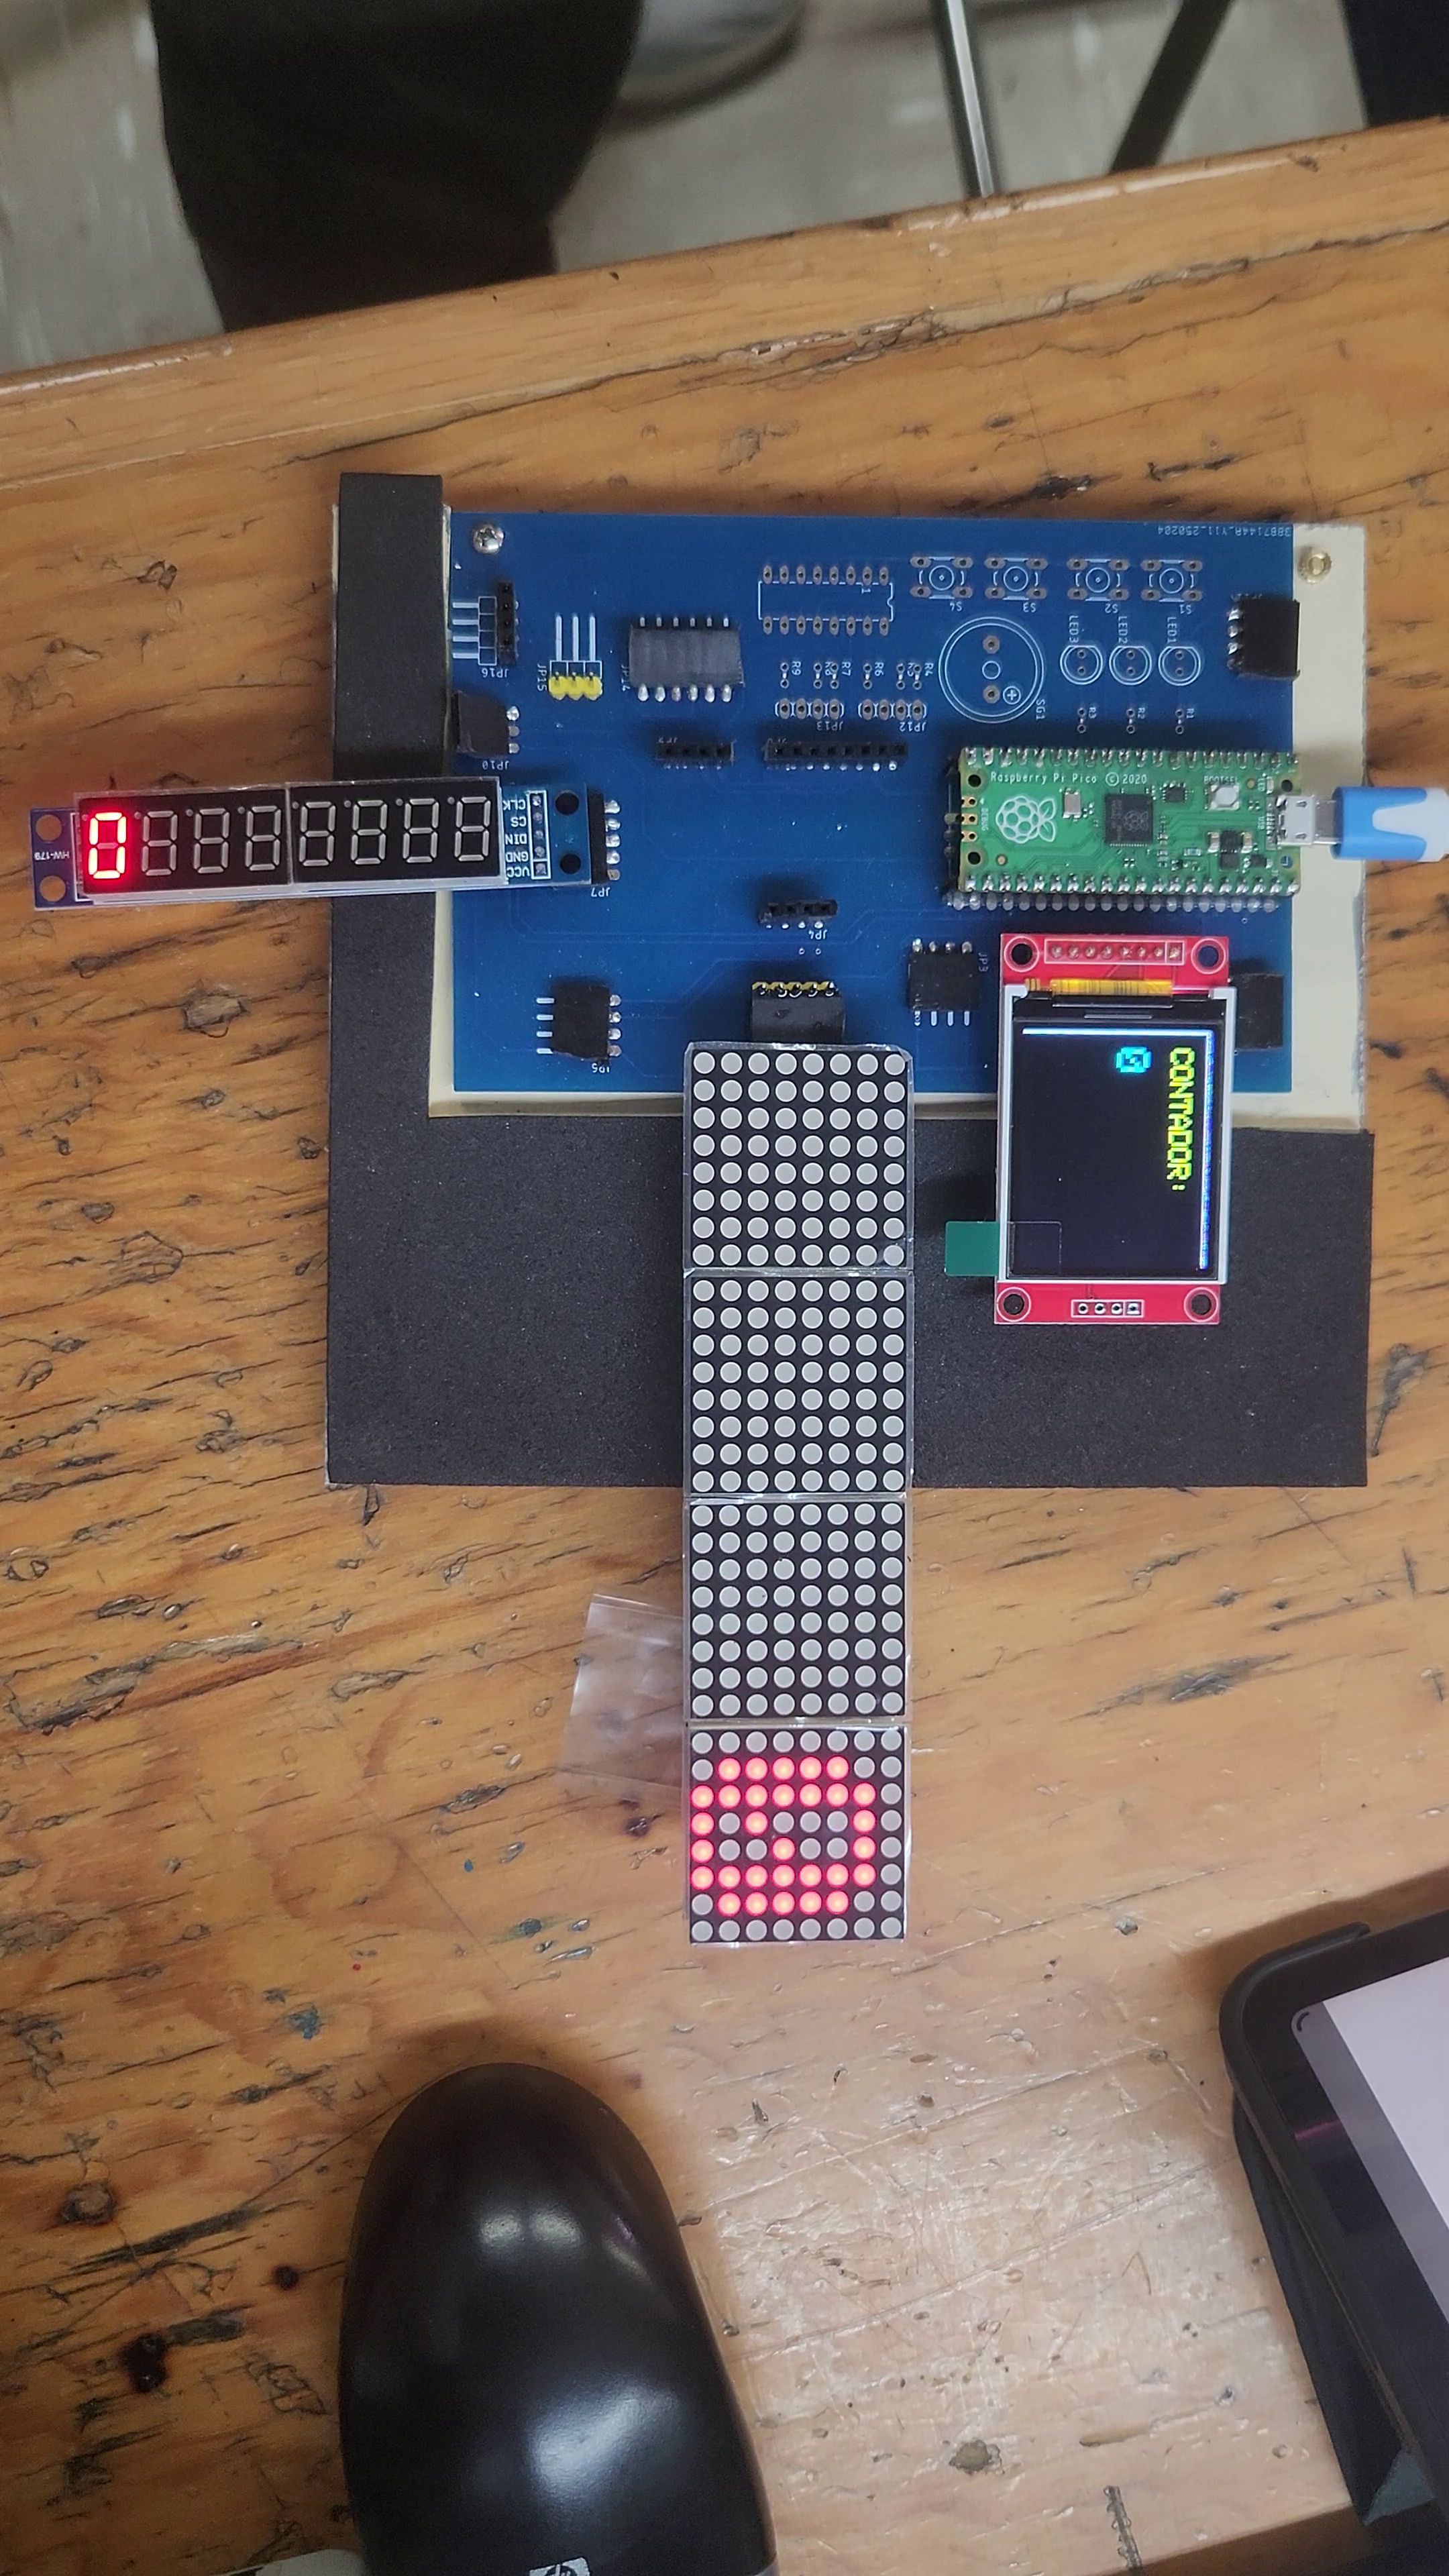
\includegraphics[width=0.4\textwidth, angle=-90]{img/Actividad7/Act7_7.png}
        \caption{Estado de inicialización ("0"). Esta captura representa la lectura del estado base del sistema (o la detención/reseteo por botón). Los tres periféricos se actualizan para reflejar la variable en cero, validando que el arbitraje de datos del RP2040 funciona desde el primer ciclo de reloj.}
    \end{figure}
    \begin{figure}[H]
        \centering
        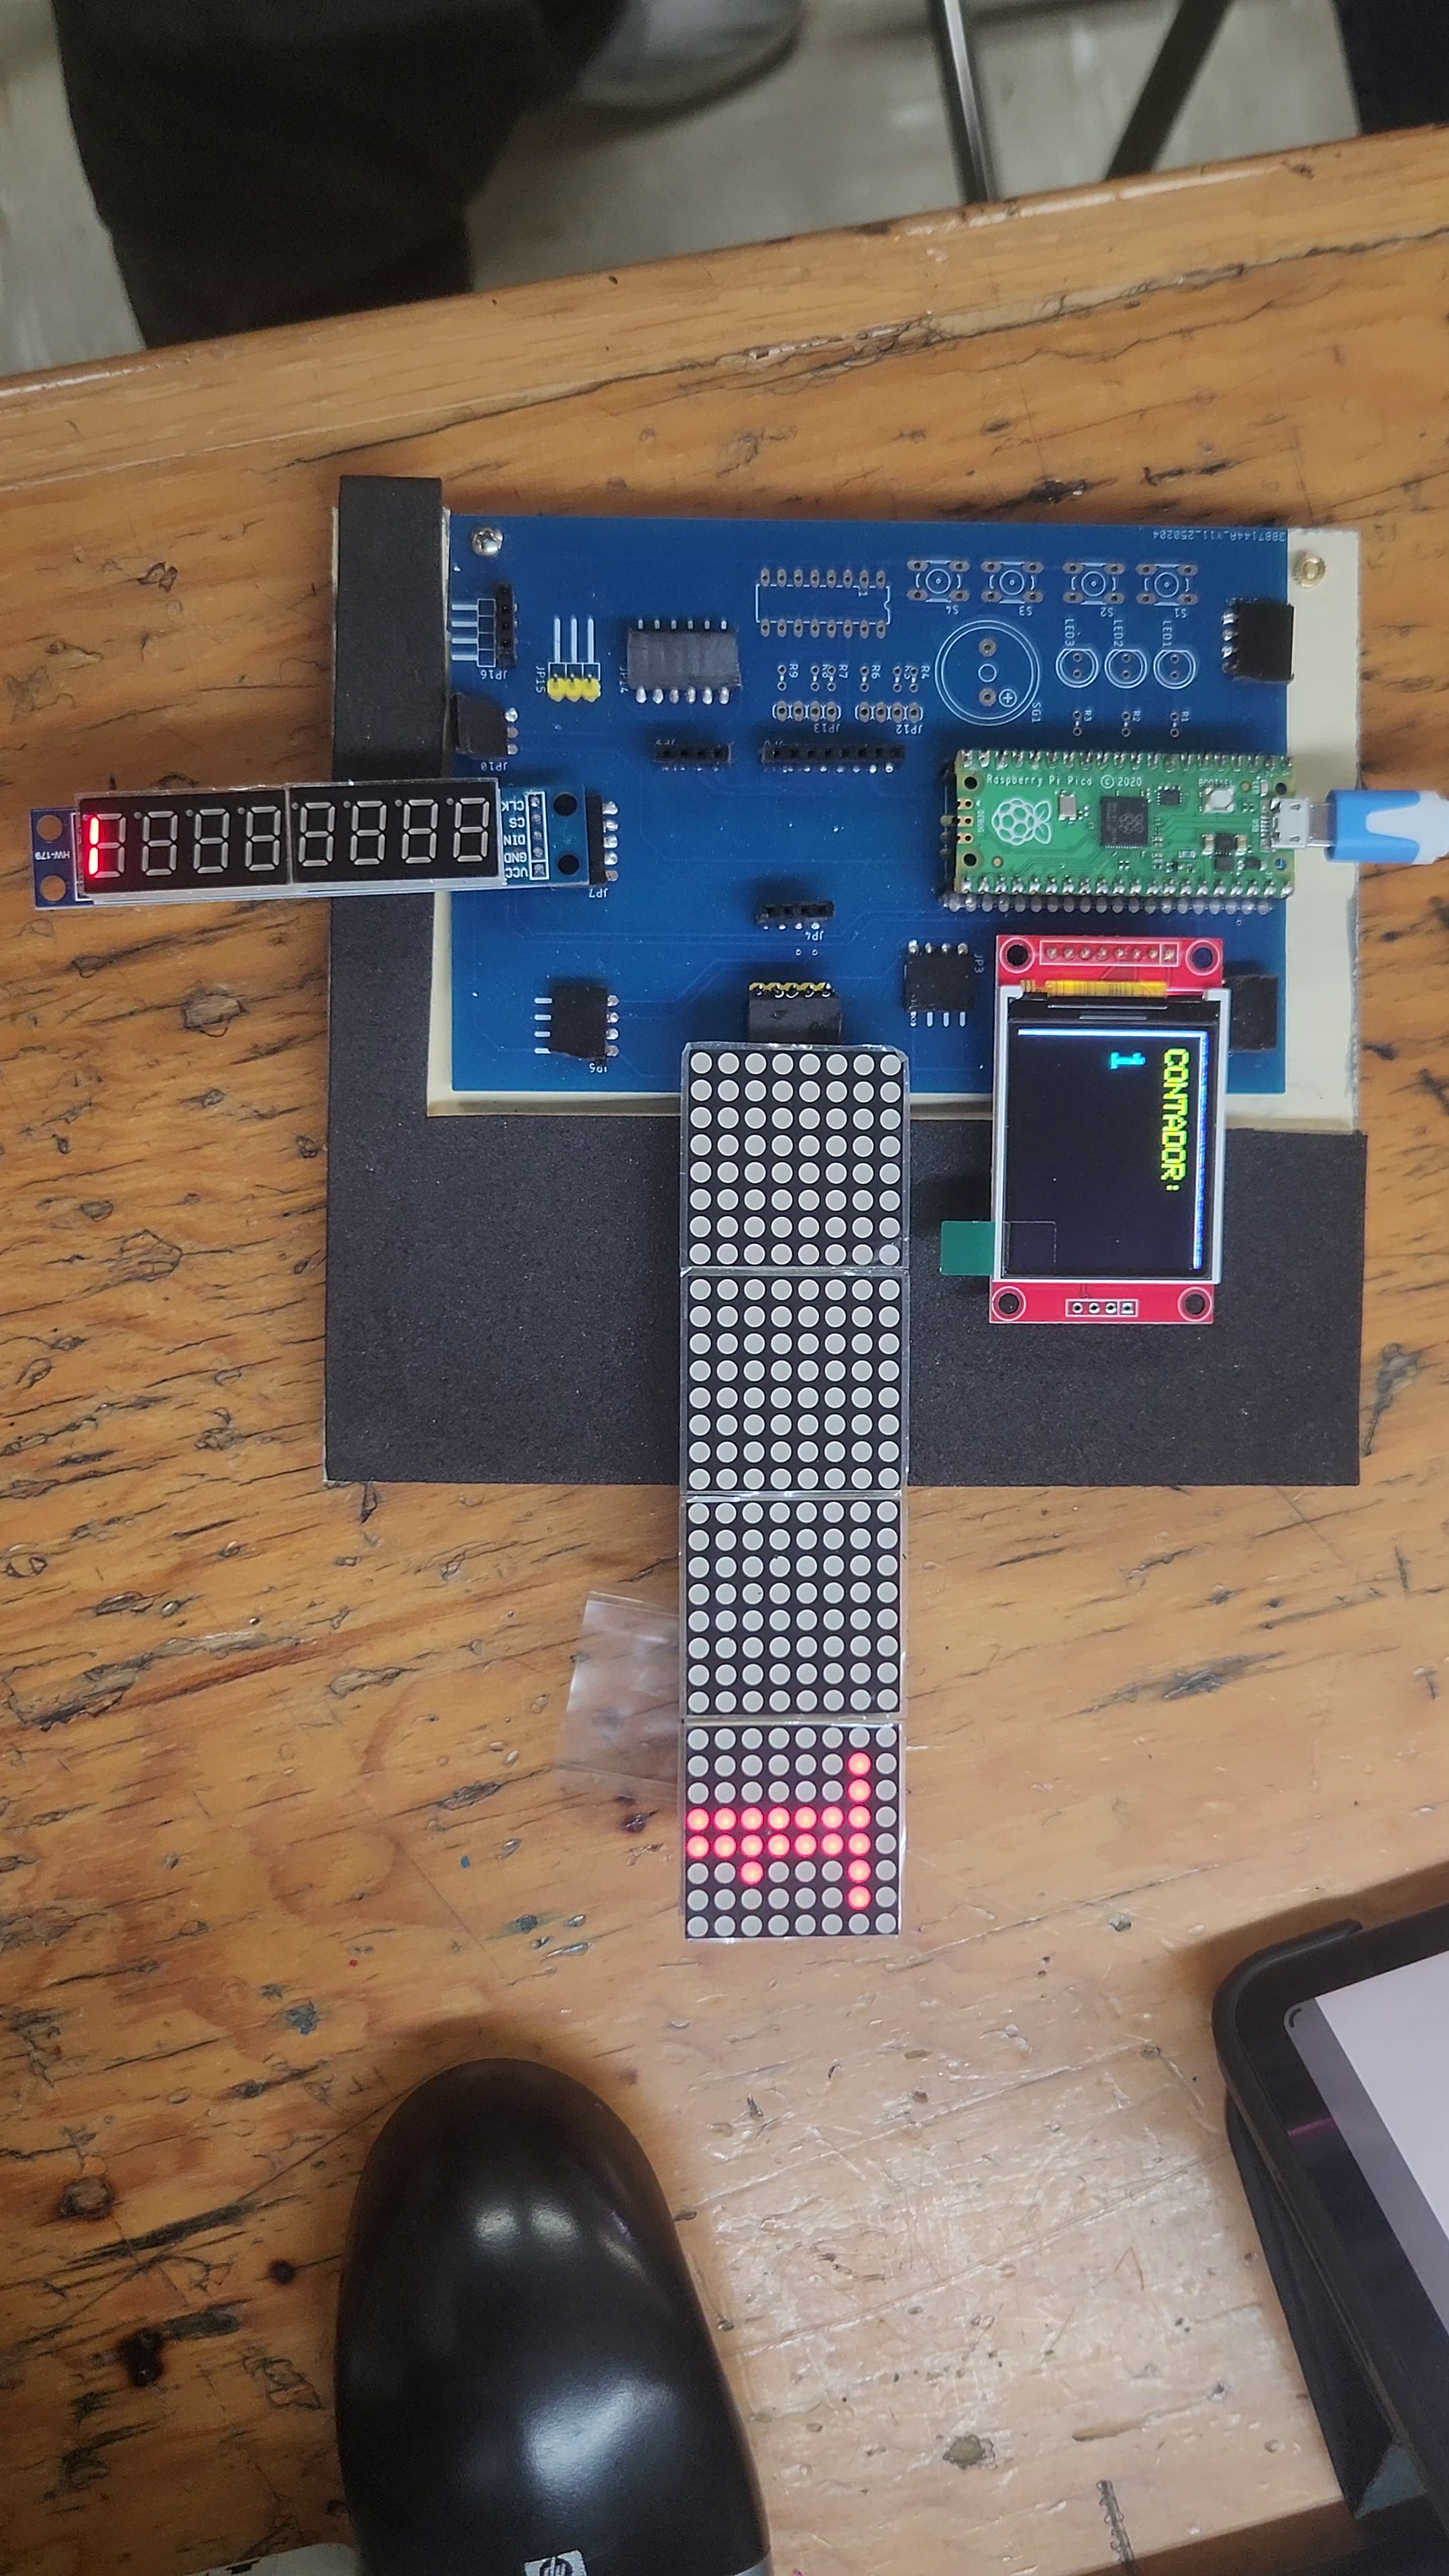
\includegraphics[width=0.4\textwidth, angle=-90]{img/Actividad7/Act7_1.png}
        \caption{Avance del contador al valor "1". El microcontrolador envía la información a través del bus SPI compartido, conmutando rápidamente los pines de selección de chip (CS) para actualizar el display de 8 dígitos, la matriz de LEDs y la pantalla TFT casi al mismo instante.}
    \end{figure}

    \begin{figure}[H]
        \centering
        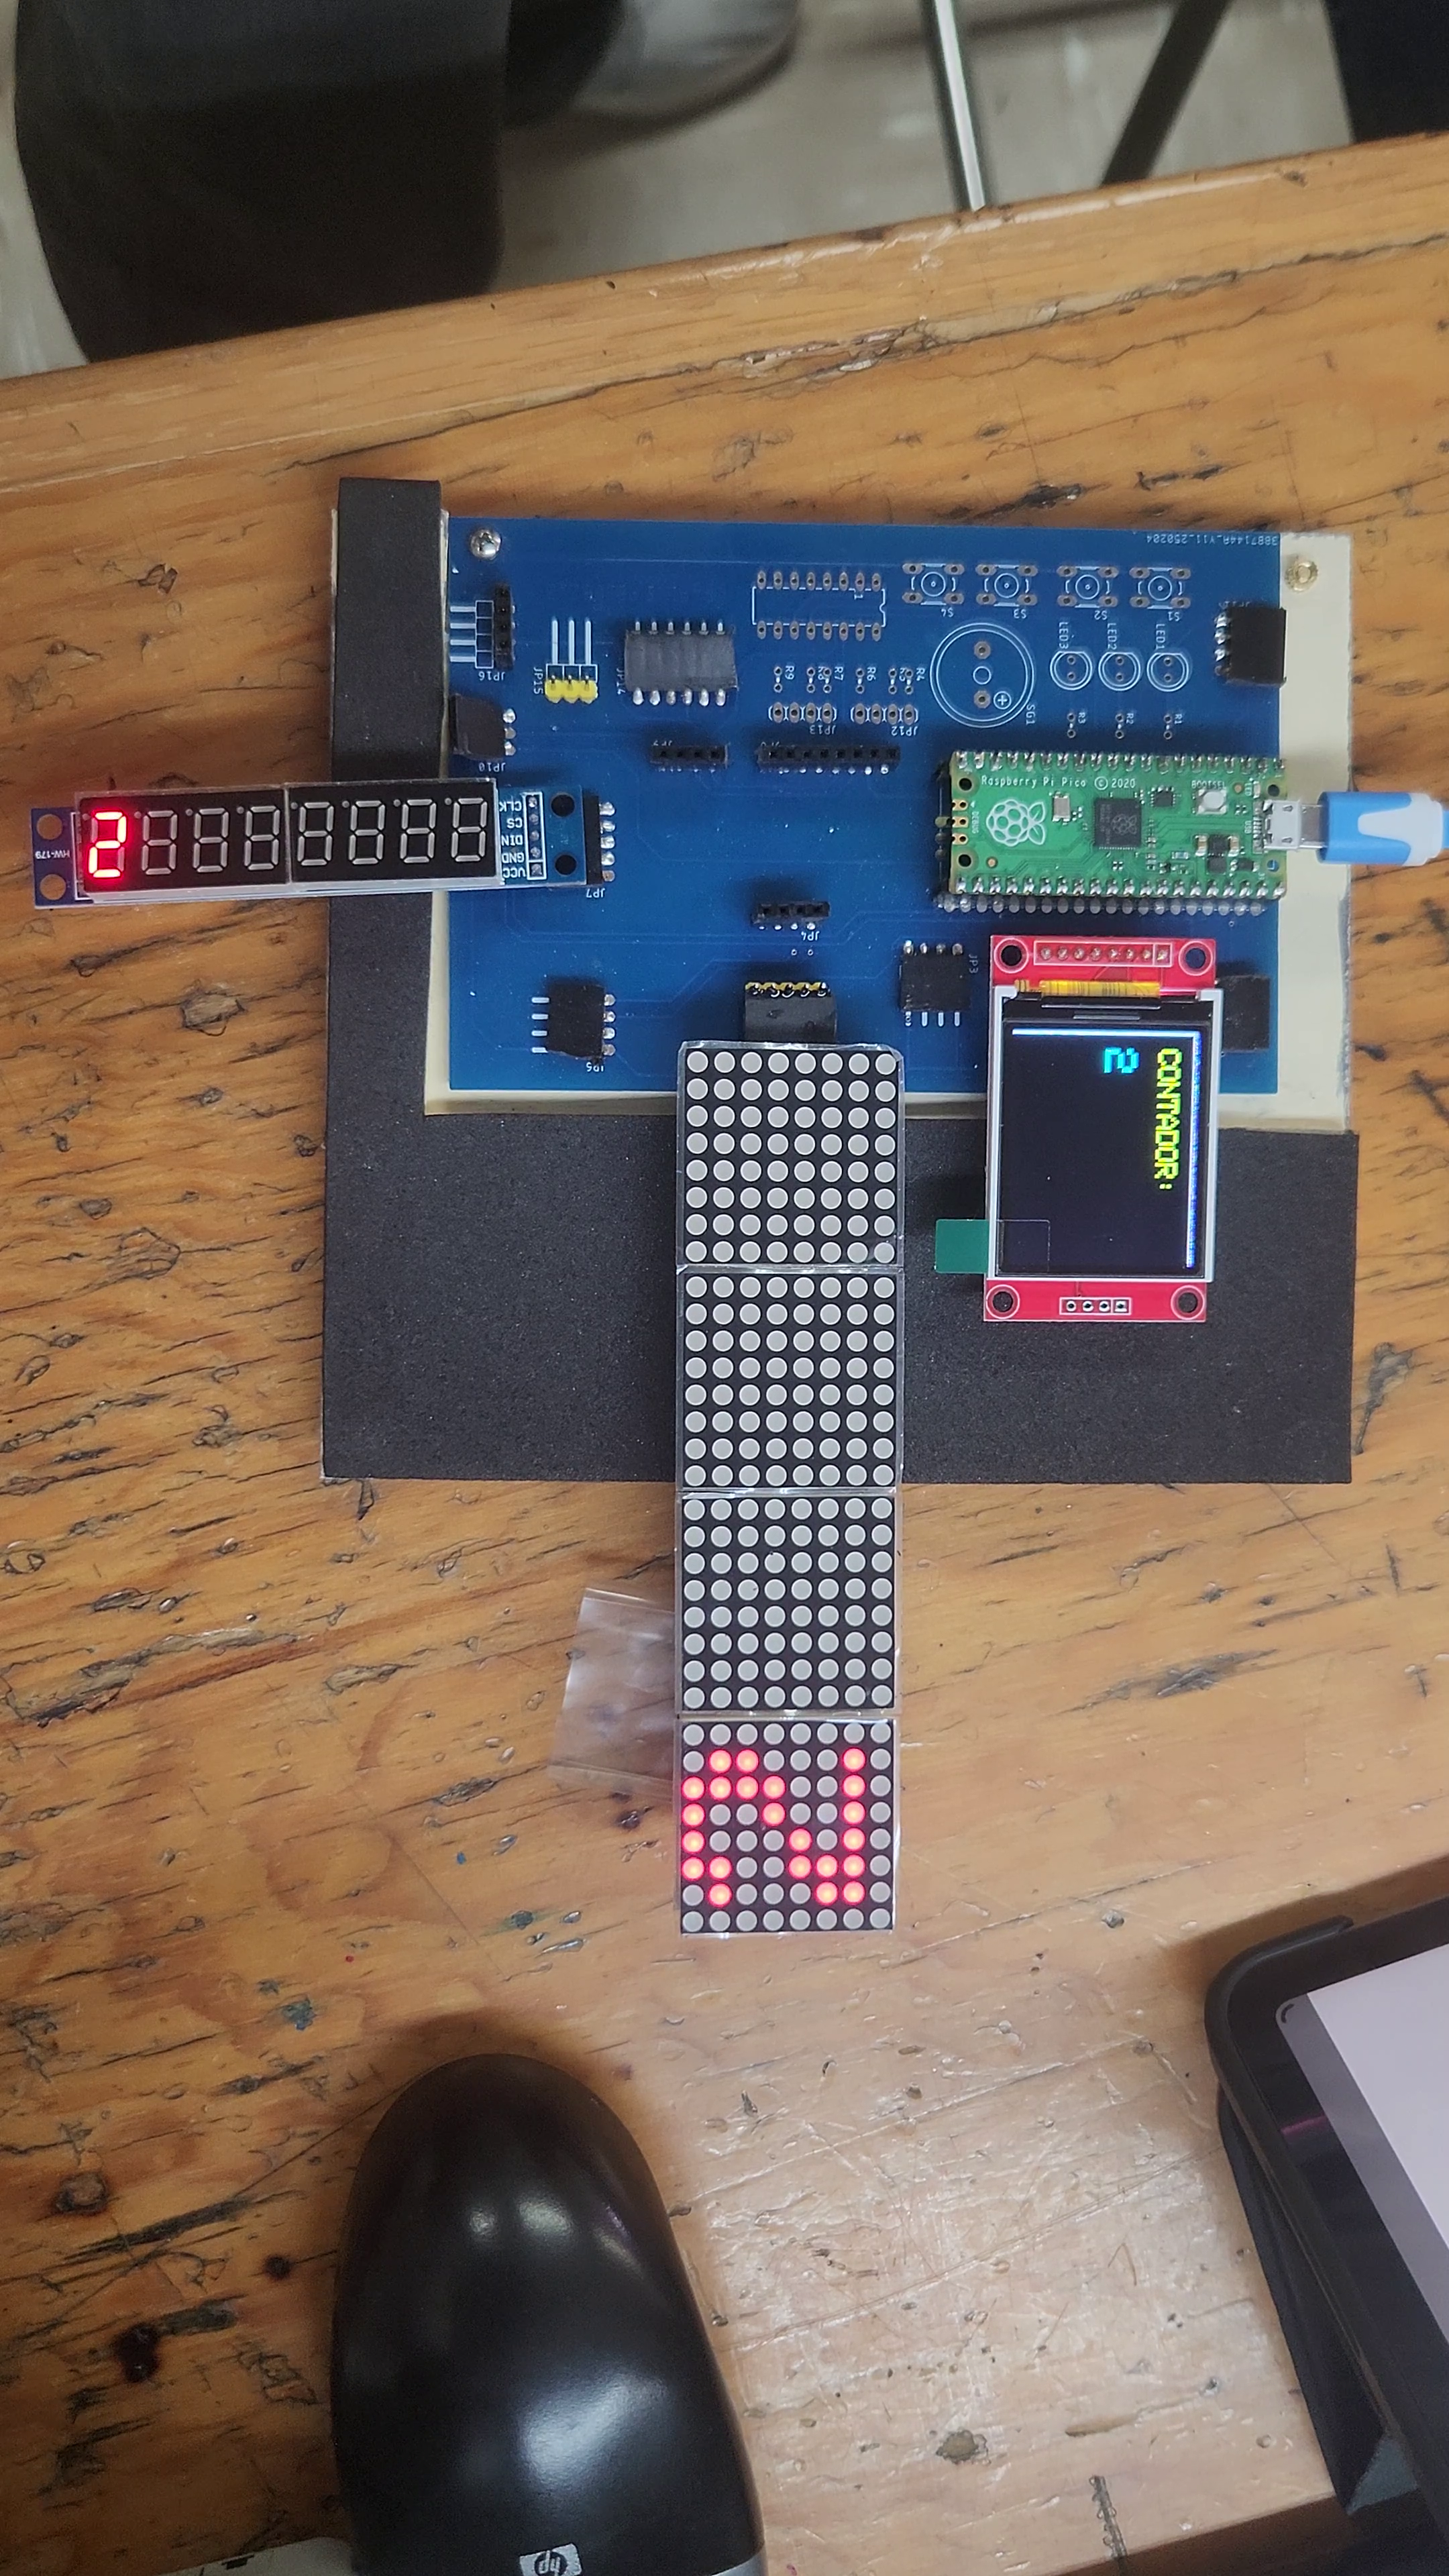
\includegraphics[width=0.4\textwidth, angle=-90]{img/Actividad7/Act7_2.png}
        \caption{Conteo en el valor "2". Se aprecia el efecto de la técnica de borrado selectivo en la pantalla TFT. El número anterior fue sobrescrito en color negro justo antes de renderizar el nuevo valor en cian, logrando una transición limpia y sin parpadeos lentos.}
    \end{figure}

    \begin{figure}[H]
        \centering
        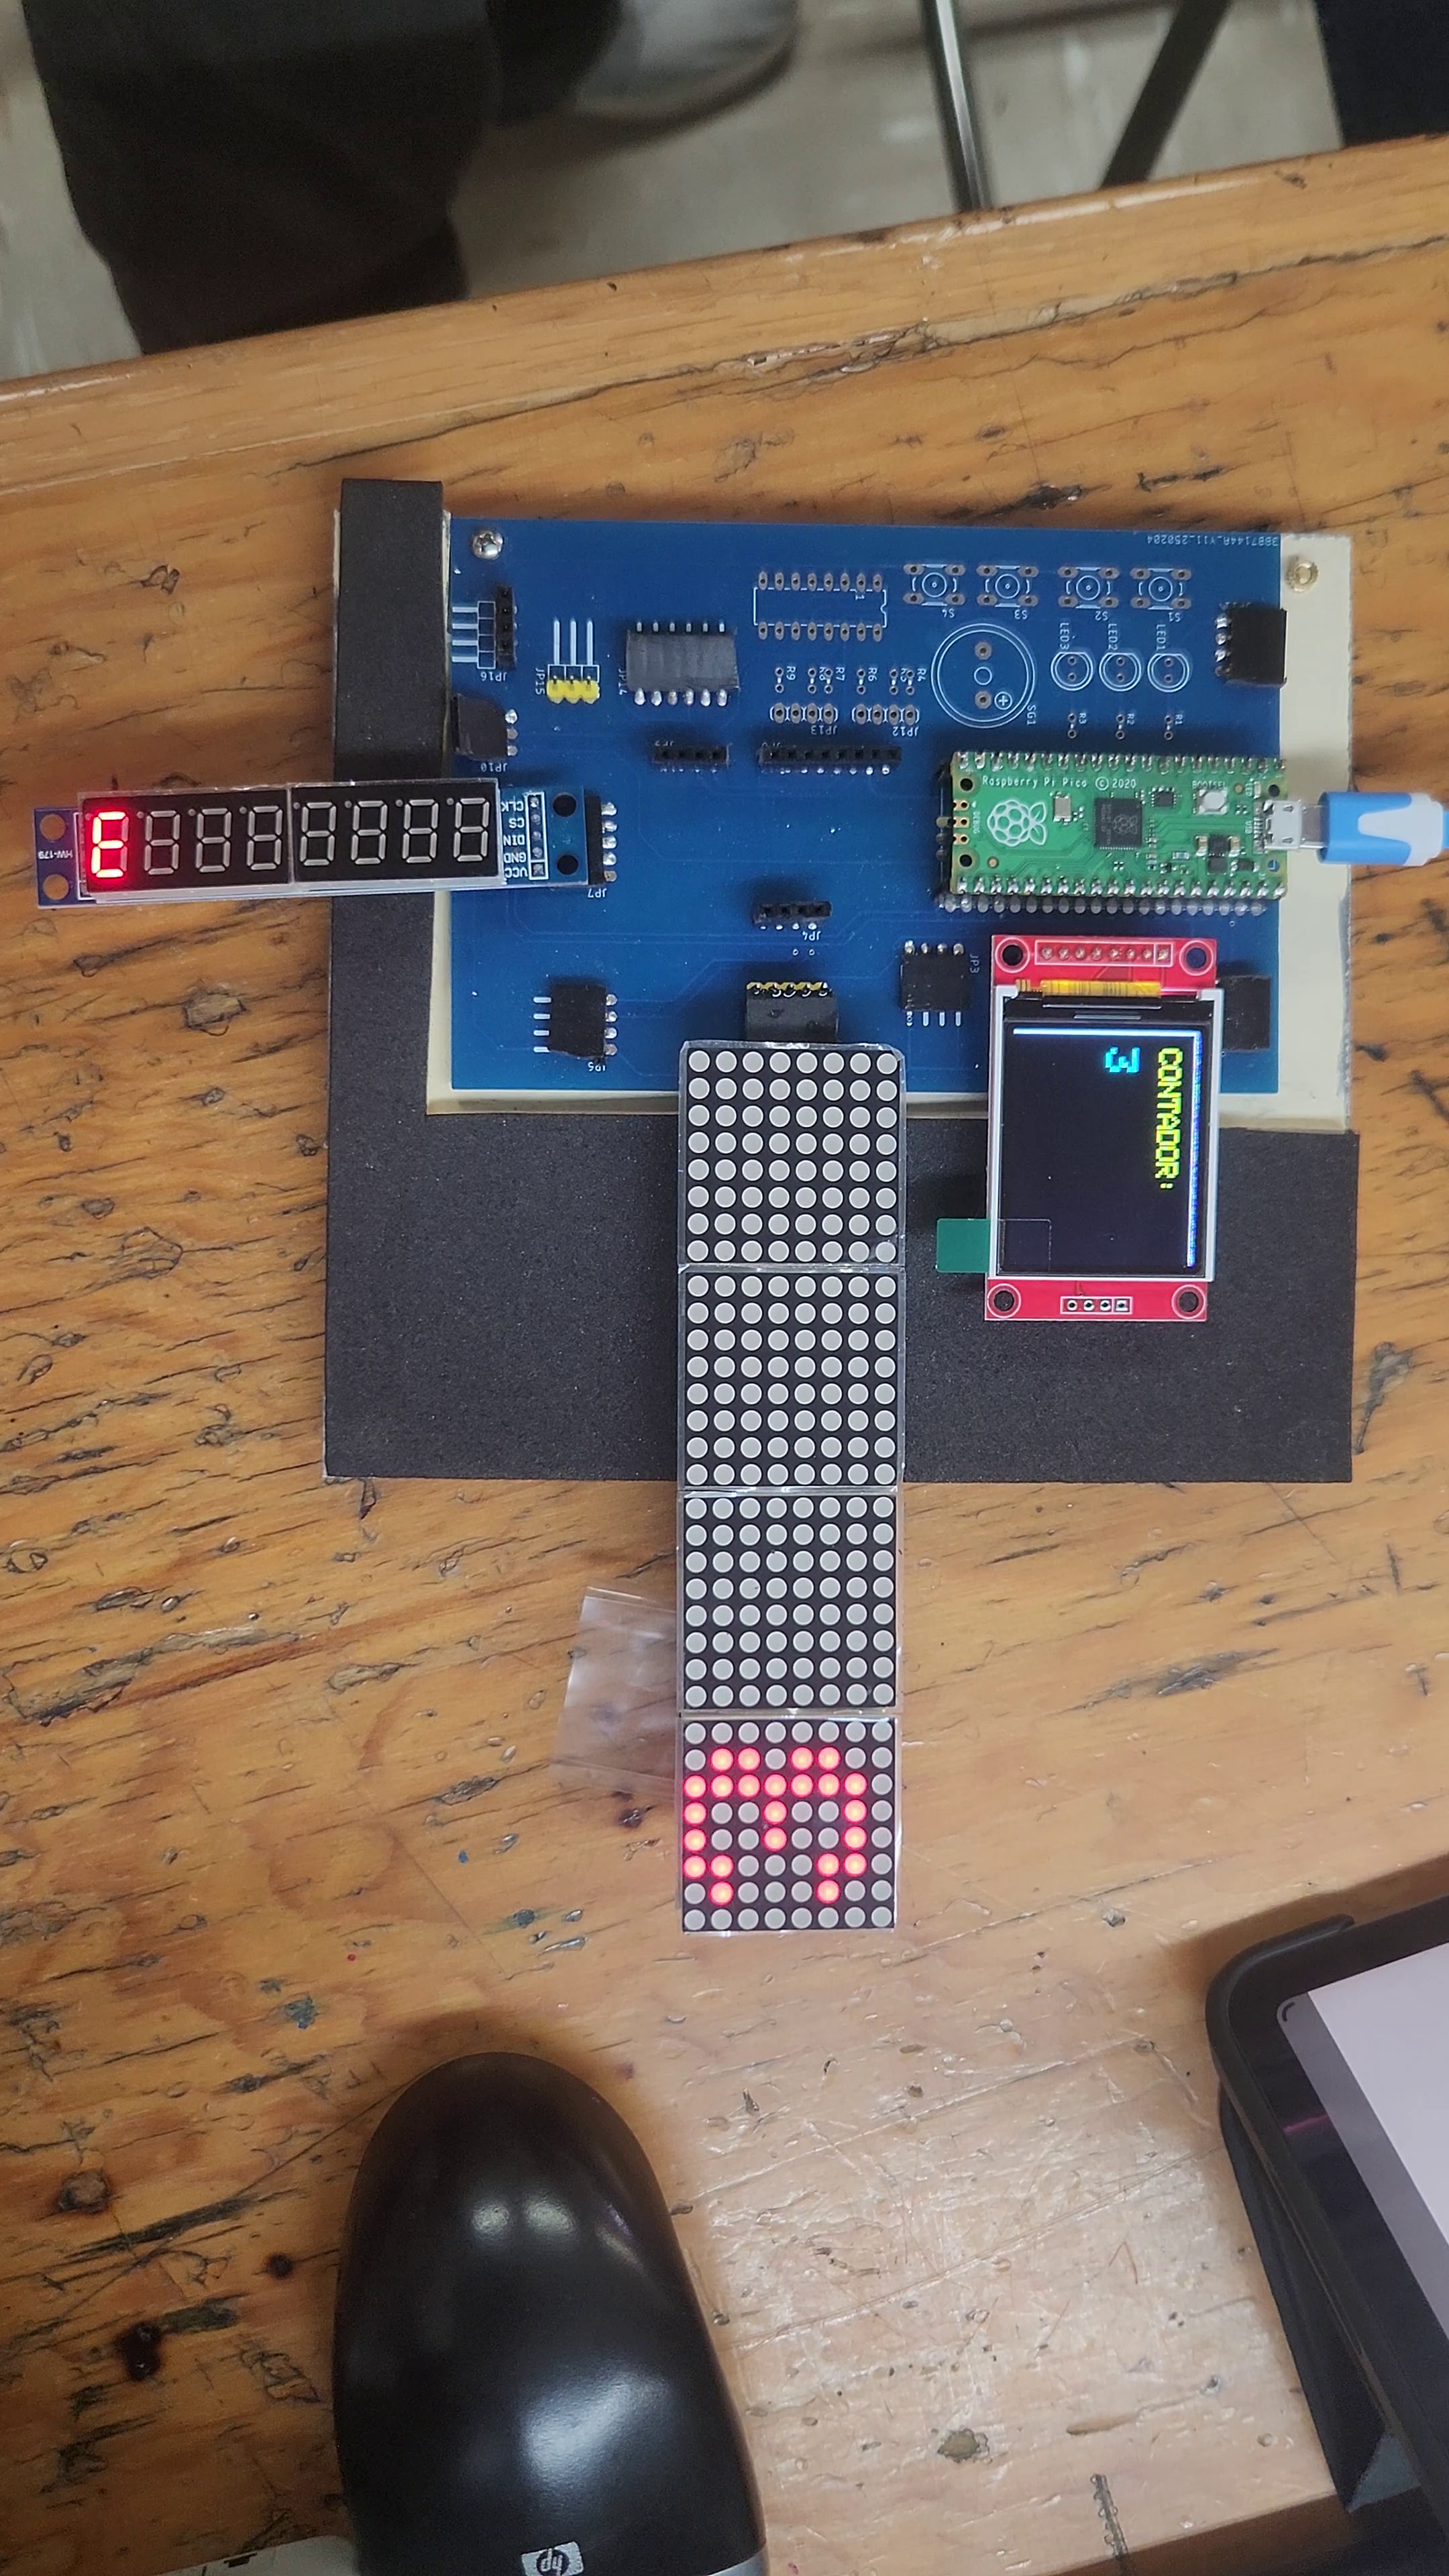
\includegraphics[width=0.4\textwidth, angle=-90]{img/Actividad7/Act7_3.png}
        \caption{Conteo en el valor "3". Los controladores MAX7219 dedicados a la matriz y al display de 7 segmentos procesan las tramas de datos de forma paralela al panel gráfico a color, demostrando la ausencia de latencia visual entre las tres arquitecturas físicas.}
    \end{figure}

    \begin{figure}[H]
        \centering
        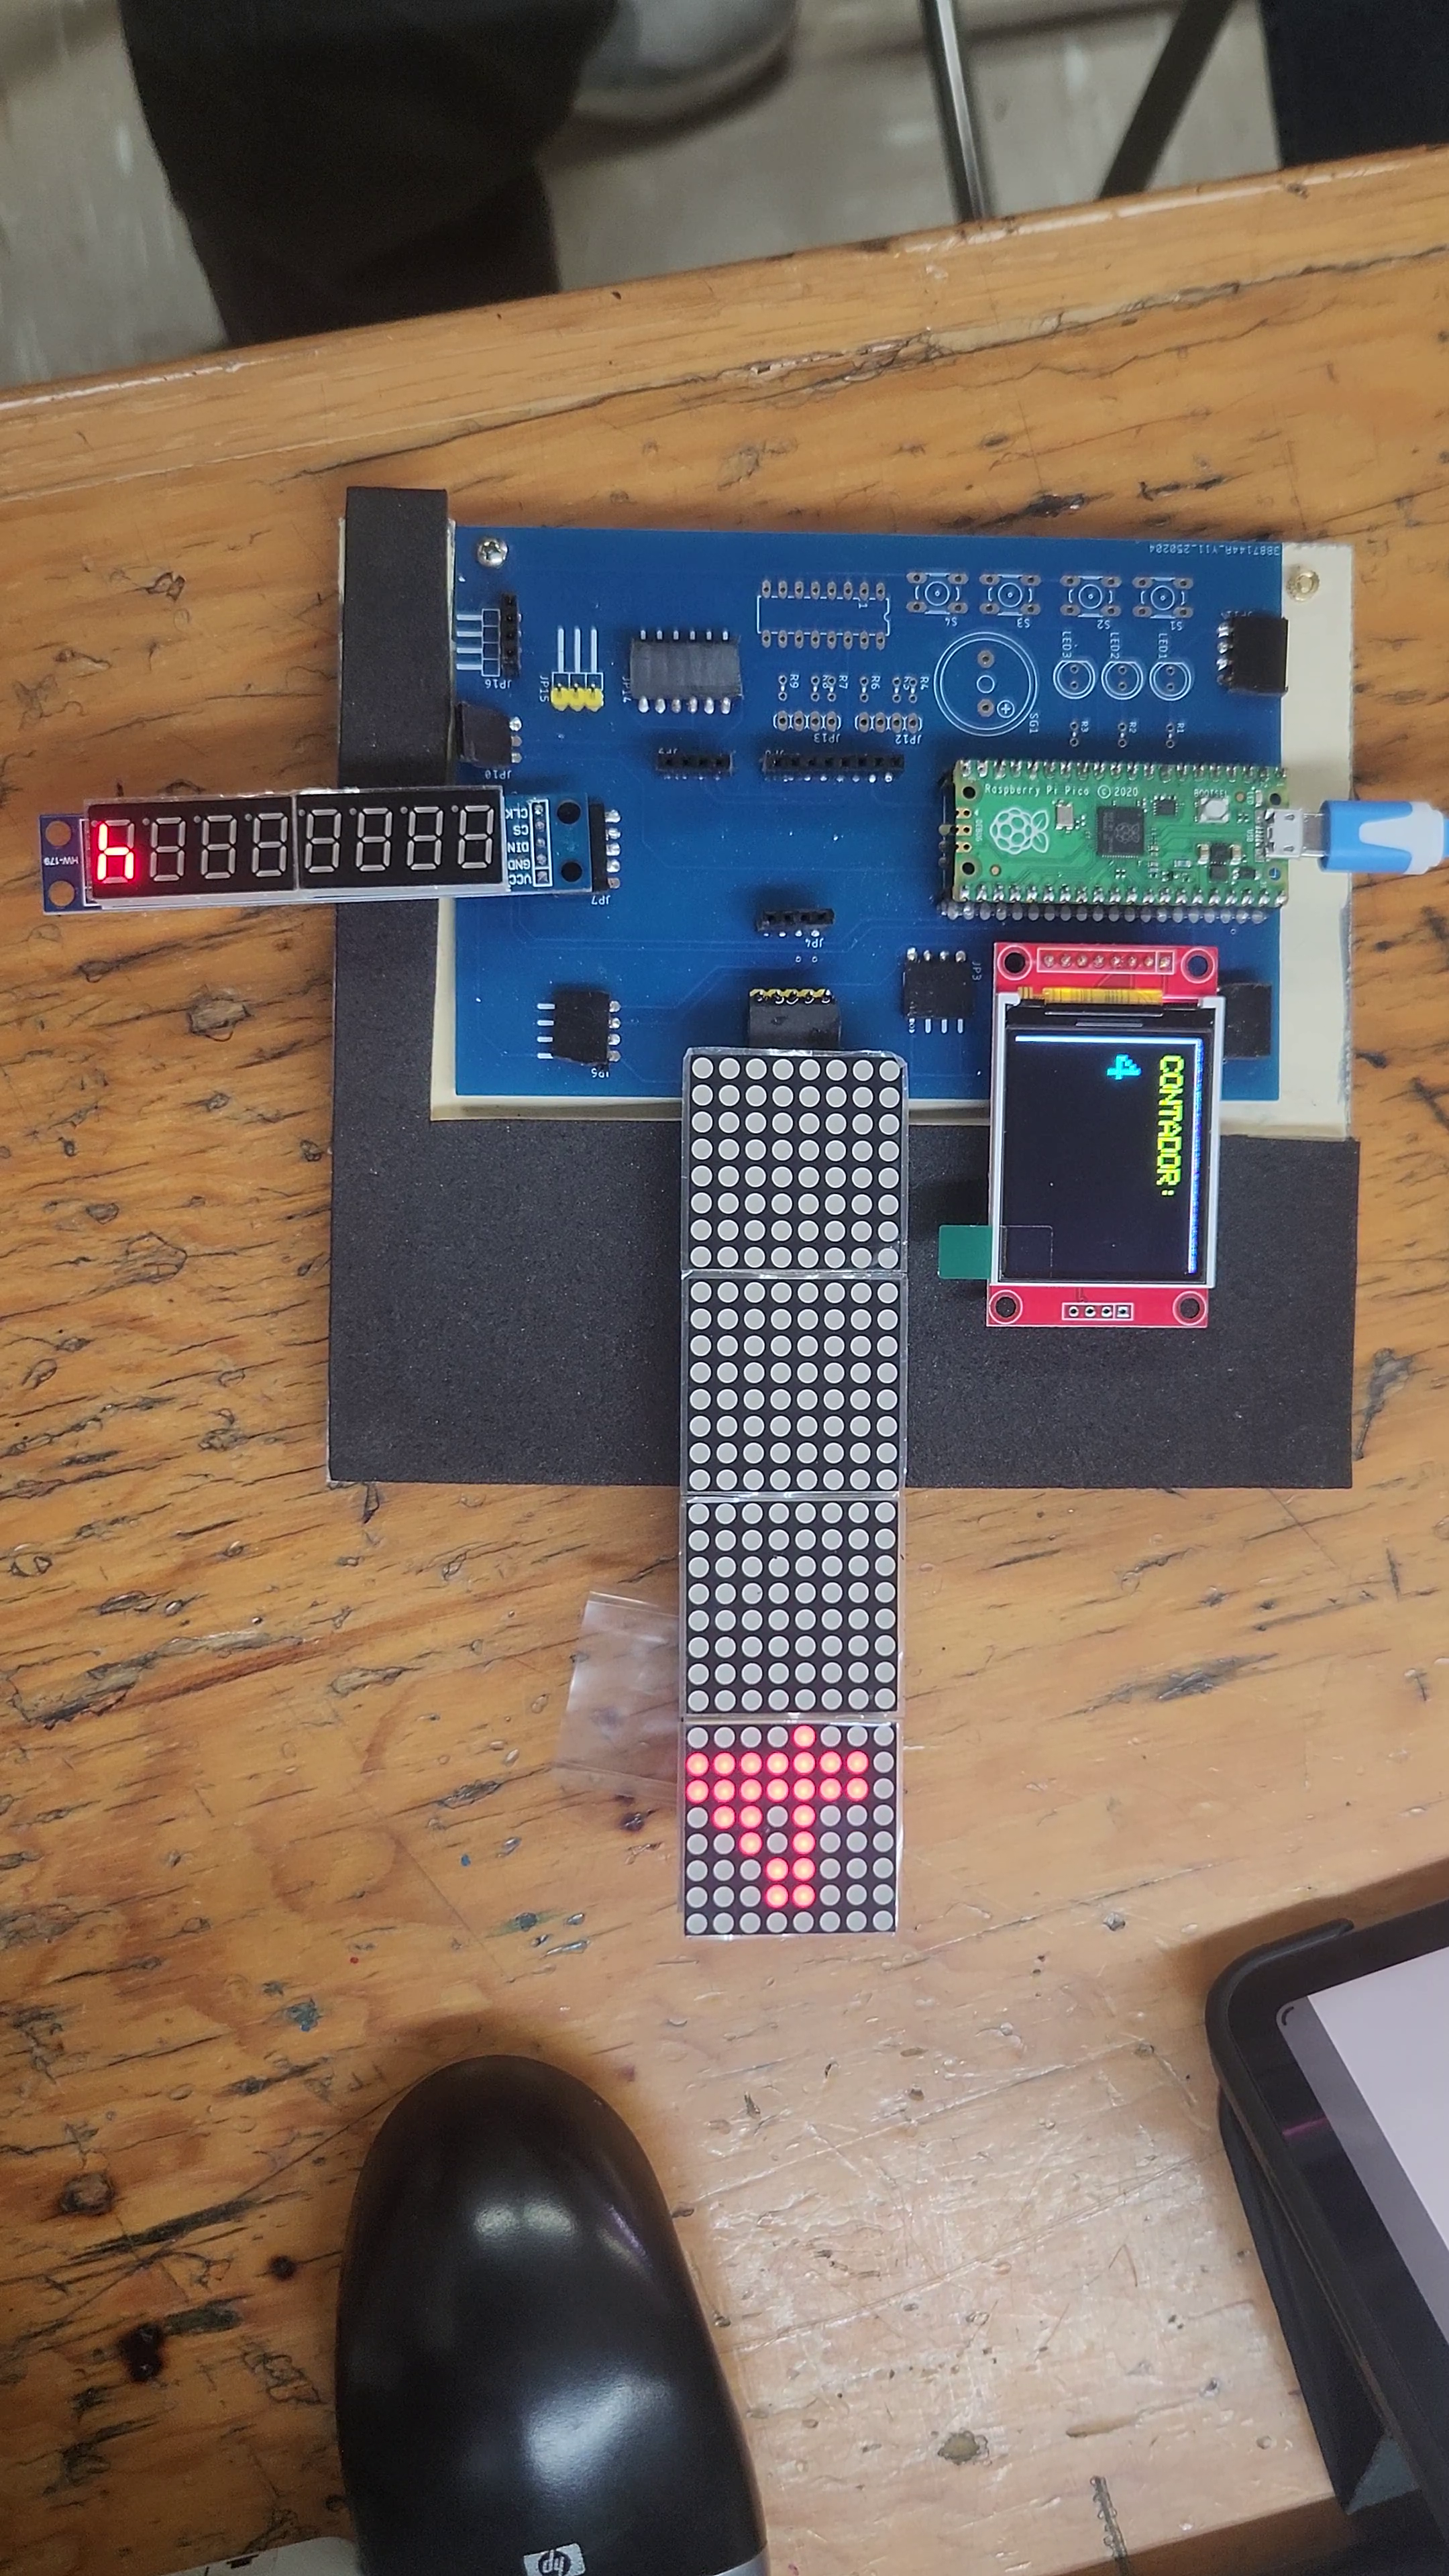
\includegraphics[width=0.4\textwidth, angle=-90]{img/Actividad7/Act7_4.png}
        \caption{Conteo en el valor "4". El formato de cadena configurado en el código (\texttt{"\{:8d\}"}) se hace evidente en el display superior, empujando numéricamente el dígito hacia el extremo derecho, mientras que en la matriz y el TFT se respeta la impresión por coordenadas absolutas.}
    \end{figure}

    \begin{figure}[H]
        \centering
        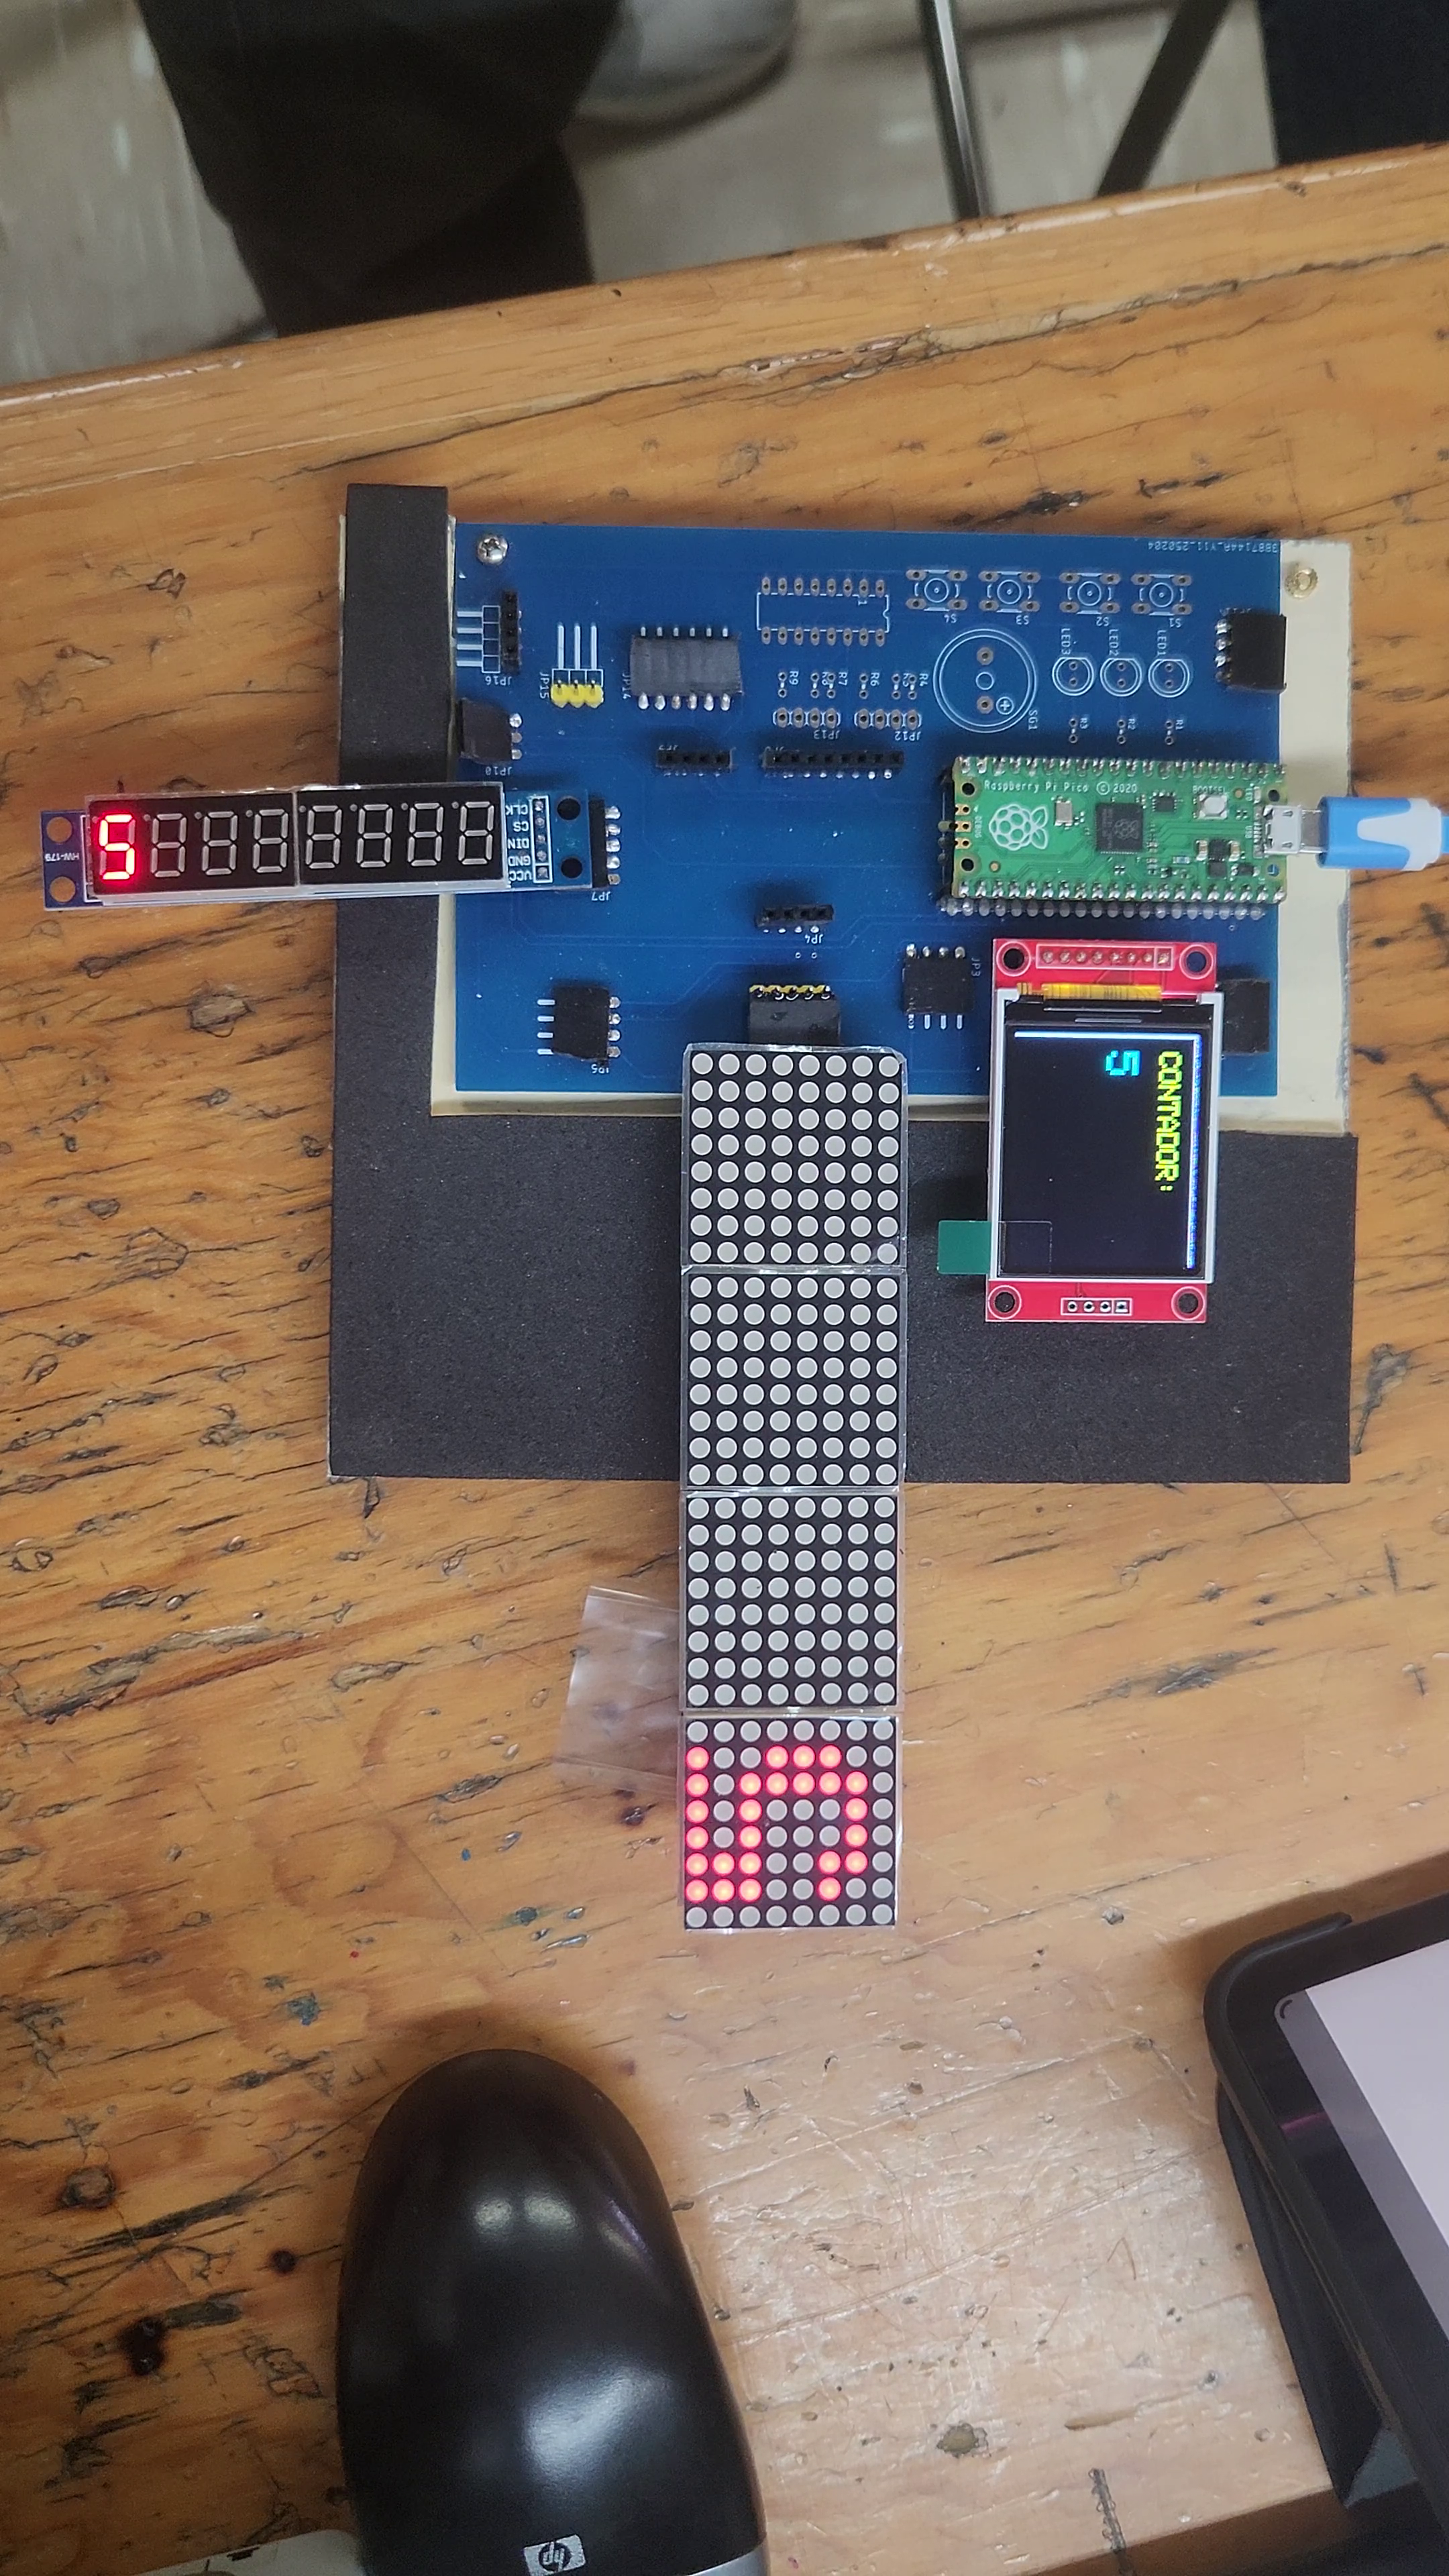
\includegraphics[width=0.4\textwidth, angle=-90]{img/Actividad7/Act7_5.png}
        \caption{Conteo en el valor "5". La ejecución continua confirma la estabilidad del bus SPI operando a 10 MHz. A pesar de comunicarse secuencialmente con tres esclavos distintos en cada ciclo, el procesador mantiene un flujo constante sin cuellos de botella.}
    \end{figure}

    \begin{figure}[H]
        \centering
        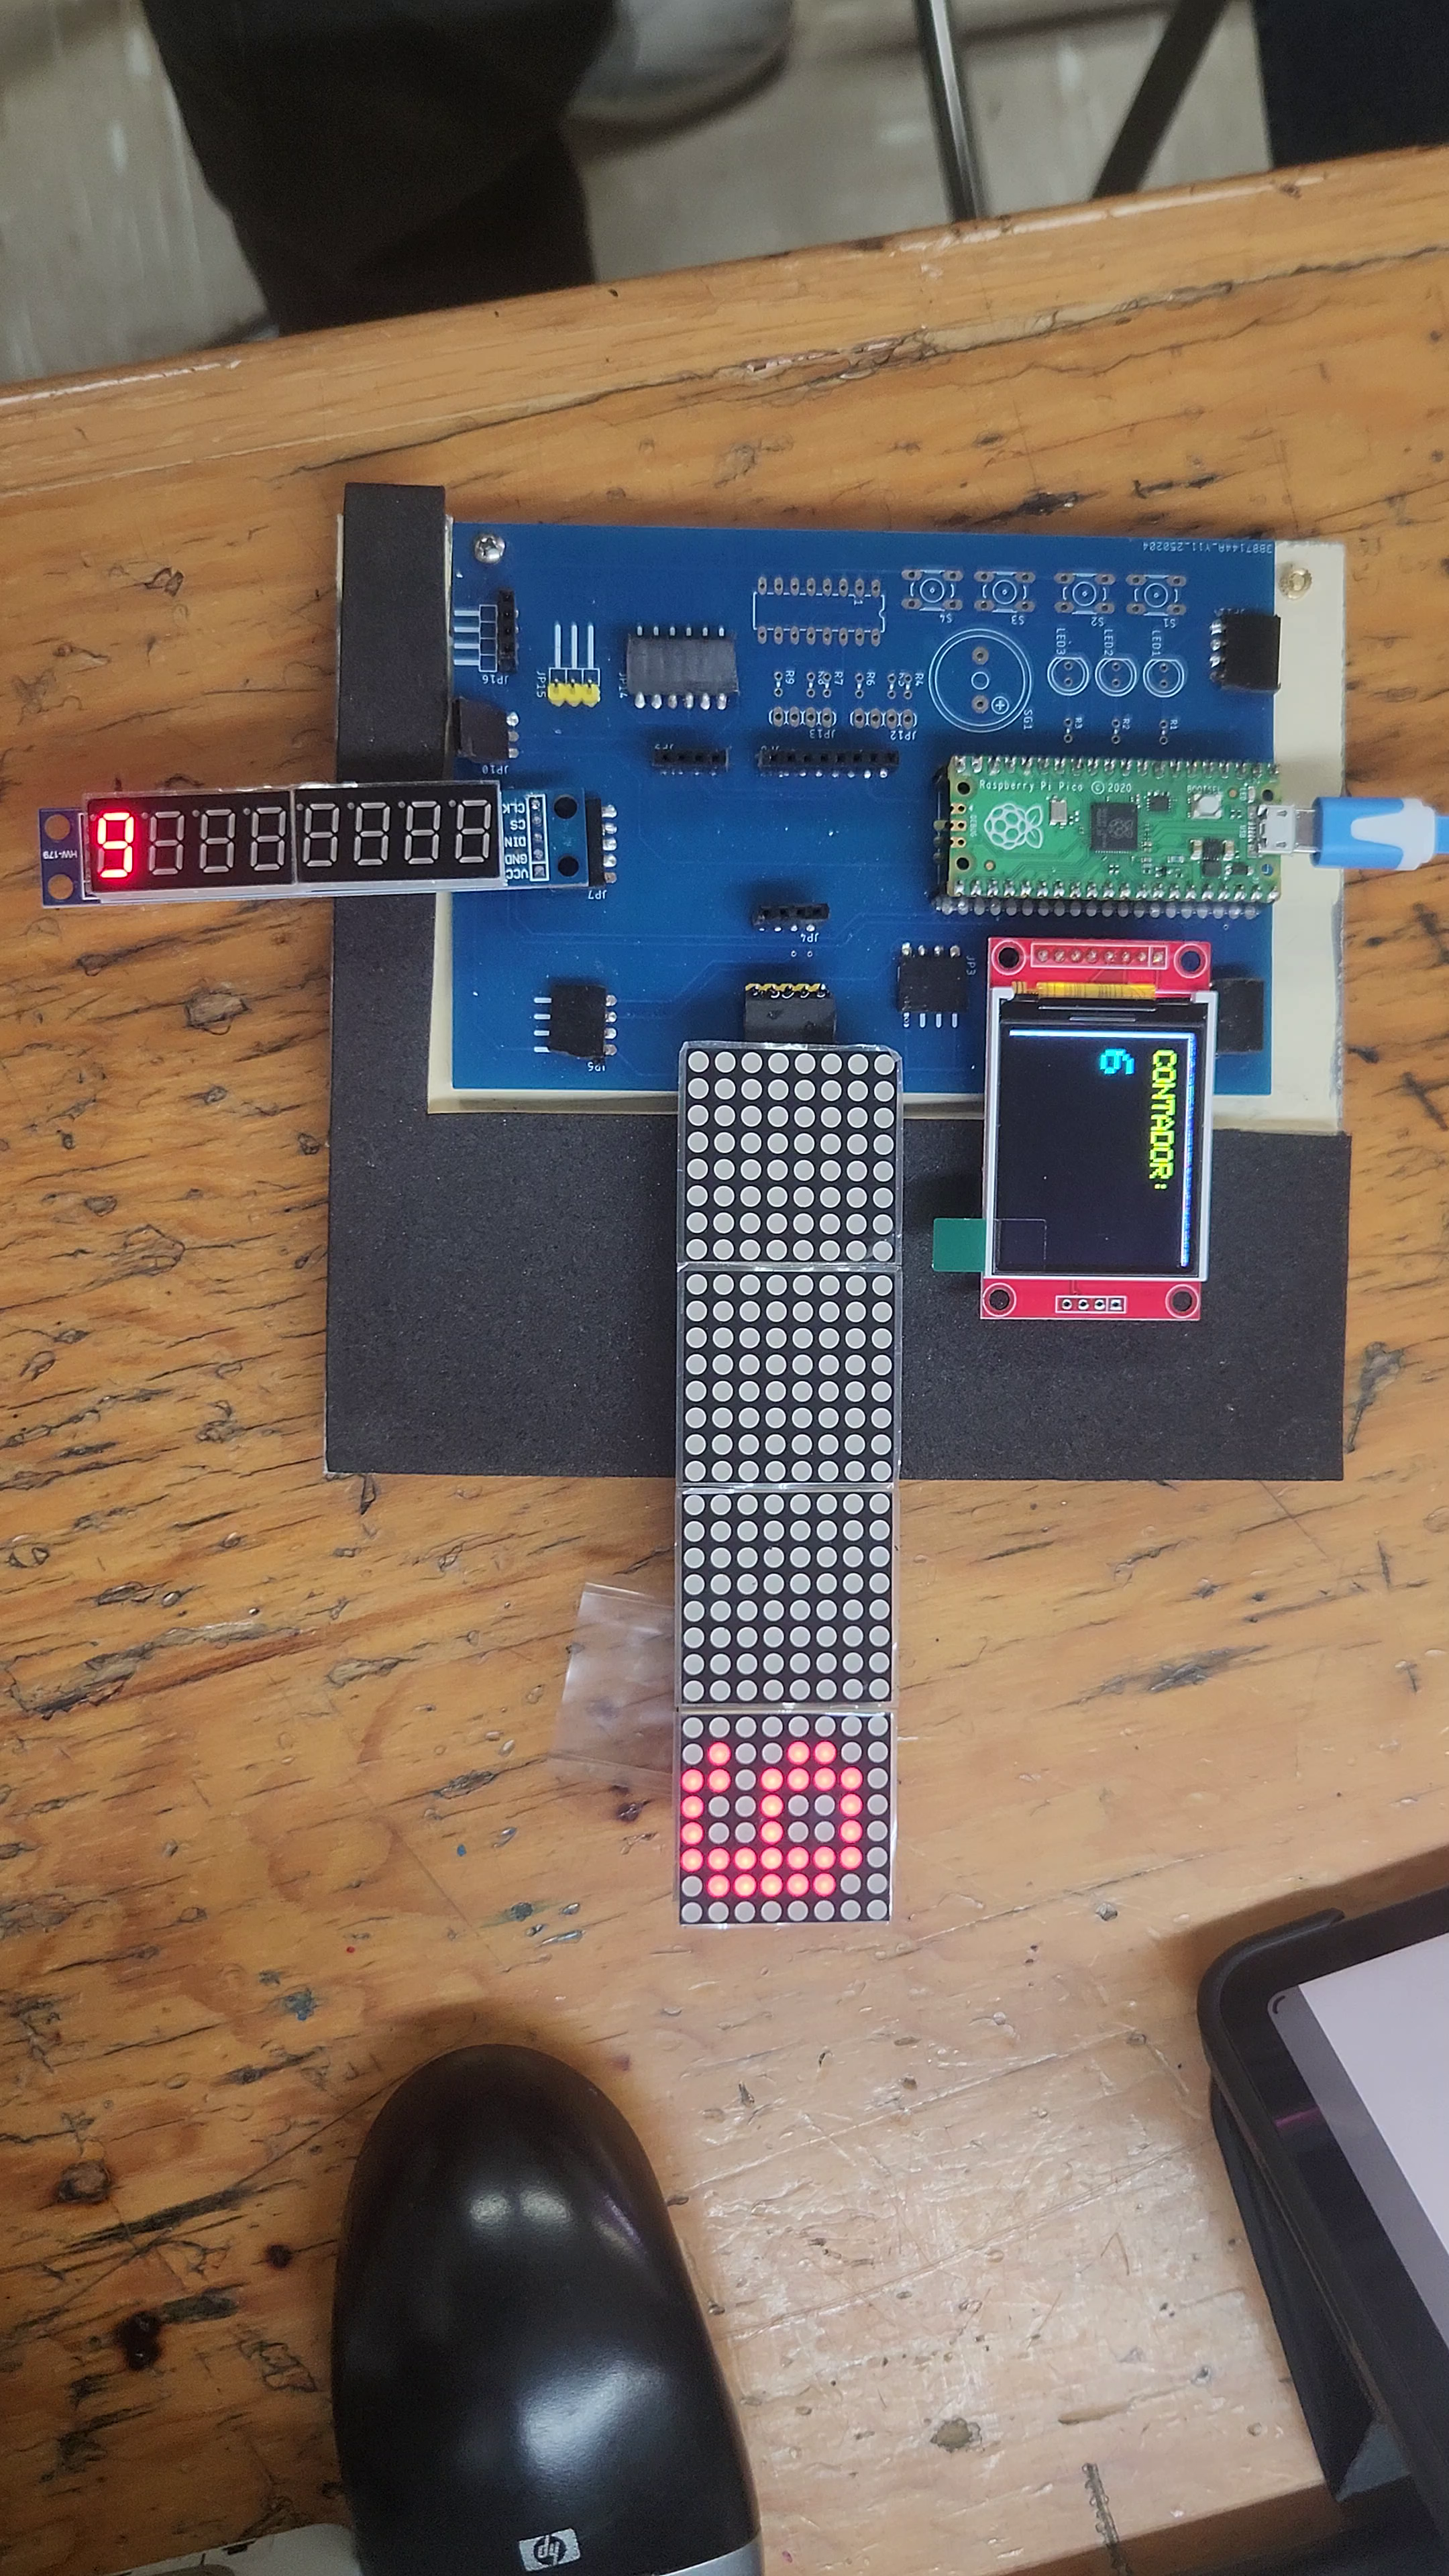
\includegraphics[width=0.4\textwidth, angle=-90]{img/Actividad7/Act7_6.png}
        \caption{Conteo en el valor "6". El avance numérico fluye de manera natural respetando el retardo programado de 0.5 segundos en el código principal, lo que comprueba que la bandera lógica \texttt{corriendo} opera de forma correcta al liberar la pausa del sistema.}
    \end{figure}

    \subsection*{Análisis de resultados}
    El código demuestra en la práctica cómo funciona el arbitraje en el protocolo SPI con múltiples esclavos. A nivel de hardware, los tres módulos reciben continuamente la misma señal de reloj y los mismos trenes de datos. Sin embargo, las librerías bajan el voltaje a 0V únicamente en el pin CS del periférico al que va dirigida la instrucción en ese momento exacto. Esto hace que el módulo seleccionado lea la información mientras los otros dos la ignoran por completo, permitiendo actualizar las tres pantallas casi al instante y sin mezclar los datos.

    Al entrar en el bloque \texttt{if corriendo:}, el contador aumenta su valor. La matriz recibe el dato convertido a texto directo, el display de 8 dígitos lo recibe con formato de espaciado (\texttt{"\{:8d\}"}), y el TFT lo posiciona gráficamente. Un punto técnico destacable es la optimización gráfica en la pantalla a color: en lugar de usar \texttt{tft.fill()} para limpiar toda la pantalla en cada número —lo cual causaría un parpadeo constante y lento—, el programa imprime el número actual en color \texttt{CYAN}, espera un momento y luego reescribe exactamente el mismo número pero en color \texttt{BLACK}. 
    Esto actúa como una goma de borrar localizada, dejando el espacio listo para el siguiente dígito y asegurando que la cuenta avance de manera rápida y fluida en los tres dispositivos a la vez.


    \newpage
    \section{Conclusiones:}

    \begin{itemize}
        \item \textbf{Espinoza Matamoros Percival Ulises:} A partir de la resolución de las actividades propuestas en esta práctica, logré tener una mejor comprensión del funcionamiento y aplicación del protocolo de comunicación SPI, ya que a partir de este protocolo se pueden controlar múltiples dispositivos, especificamente en está practica el control de diferentes displays, como el display de 8 dígitos, la matriz de LEDs y la pantalla TFT. Al implementar el código para controlar estos dispositivos, pude compredner los valores de configuración necesarios para establecer la comunicación, como la frecuencia de reloj y la asignación de pines para SCK, MOSI y MISO. Además, al trabajar con el bus SPI compartido, entendí cómo se pueden gestionar múltiples periféricos utilizando líneas de control independientes (CS) para cada dispositivo, lo que permite una comunicación eficiente sin interferencias entre ellos.
        
        Por otro lado también logré comprender la importancia de las librerías específicas para cada dispositivo, ya que estas simplifican significativamente el proceso de programación al proporcionar funciones predefinidas para inicializar los displays, configurar sus parámetros y mostrar información de manera sencilla, de forma que el usar MicroPython y las librerías adecuadas proporcionan un buen flujo de trabajo a la hora de implementar soluciones con la Raspberry Pi Pico y hardware adicional.
        

        \item \textbf{Flores Colin Victor Jaziel:} A lo largo de esta práctica número ocho he comprendido el funcionamiento del protocolo SPI como medio de comunicación síncrona para controlar múltiples dispositivos desde un solo microcontrolador y esto fue evidenciado al trabajar con diferentes módulos que fueron controlados a partir de la Raspberry. Al trabajar con el display de 8 dígitos, la matriz de LEDs MAX7219 y la pantalla TFT ST7735, pude observar cómo se comparten las líneas de reloj (SCK) y datos (MOSI), mientras que cada periférico se selecciona de manera independiente mediante su propio pin CS, evitando interferencias. También entendí la importancia de configurar correctamente parámetros como la frecuencia de reloj y la asignación de pines y finalmente, comprobé que el uso de librerías específicas como max7219\_8digit, max7219.py y ST7735 simplifica enormemente la programación, permitiendo inicializar, configurar y mostrar información en cada dispositivo con pocas instrucciones.

        \item \textbf{Lara Hernandez Angel Husiel:} En esta práctica logré integrar de forma más clara el uso del bus SPI como medio de comunicación síncrona para controlar distintos dispositivos con un mismo microcontrolador. Al trabajar con el display de 8 dígitos, la matriz MAX7219 y la pantalla TFT ST7735 entendí mejor cómo se comparten las líneas de reloj y datos, pero se mantiene el control independiente de cada periférico mediante su pin de selección de chip, lo cual hace posible que varios módulos funcionen sin interferirse entre sí.

        También me quedó más claro que las librerías dedicadas simplifican mucho la programación, porque permiten inicializar la pantalla, corregir el orden de color, orientar la imagen y escribir texto con solo unas cuantas instrucciones. 
    
    \end{itemize}

    \newpage


    \nocite{*} 
    \printbibliography[heading=bibintoc, title={Referencias}]
\end{document}